\documentclass[11pt,a4paper,headinclude=true,DIV=14,BCOR=8mm,chapterprefix,listof=totoc,twoside,openright,abstracton]{scrbook}


%% packages
\usepackage[headsepline]{scrpage2}
\usepackage[utf8]{inputenc}
\usepackage{geometry}
\usepackage{amssymb}
\usepackage{amsthm}
\usepackage{enumerate}
\usepackage{graphicx}
\usepackage{float}
\usepackage[intlimits]{amsmath}
\usepackage{xcolor}
\usepackage{verbatim}
\usepackage{appendix}
\usepackage{hyperref}
\usepackage{hyperref}
\usepackage{mathtools}
\usepackage{natbib}
\usepackage{xr}
\usepackage{wrapfig}
\usepackage[framemethod=tikz]{mdframed} % for a block of text
\usepackage{etoolbox}

%% properties
\setlength{\parindent}{0pt}
\setcitestyle{aysep={}} 
\bibliographystyle{apalike}
\setcitestyle{citesep={,}}
\newtoggle{Full}
\togglefalse{Full}
\geometry{a4paper, tmargin=3cm, bmargin=3cm, lmargin=3cm, rmargin=3cm, headheight=3em, headsep=2em, footskip=1cm}

%% commands / macro
\newcommand{\todo}[1]{\textcolor{red}{$\blacksquare$ TODO: #1}} 
\newcommand{\red}[1]{\textcolor{red}{#1}} 
\newcommand{\gray}[1]{\textcolor{gray}{#1}} 
\newcommand{\magenta}[1]{\textcolor{magenta}{#1}} %% For terms/concepts to remember 
\newcommand{\swind}{spiral-wave wind}
\newcommand{\nwind}{$\nu$-component}
\newcommand{\gcm}{g cm$^{-3}$}
\newmdenv[linecolor=cyan,backgroundcolor=cyan!20]{sidenote}

%% head
\title{PhD thesis}
\author{Vsevolod Nedora}
\date{today}


%% ==================== START ================
\begin{document}

\maketitle

\mainmatter

%% ================= Targeted structure ====
%%
%% Part 1: Numerical relativity simulations of neutron star mergers
%%         Ch.1. Introduction
%%         Ch.2. Theoretical Background
%%               Sec.1. General-relativistic hydrodynamics
%%               Sec.2. Numerical Approximations of conservation laws
%%               Sec.3. High order numerical methods for Rel.Hydro.
%%               Sec.4. Relativistiv Radiation transport
%%               Sec 5. Microphysical equation of starts of nuclear matter
%%         Ch.3. Numerical relativity simulations
%%               Sec.1. Evolution code and Initial Data code
%%               Sec.2. Data analysis methods
%%         Ch.4. Results and Conclusions
%% Part 2: Electromagnetic counterparts to neutron star mergers
%%         Ch.1. Introduction
%%         Ch.2. Theoreticak Background
%%               Sec.1. Nucleosynthesos in binary neutron star ejecta
%%               Sec.2. Kilonova
%%               Sec.3. Short Gamma Ray Burst afterglow
%%               Sec.4. Ejecta aftergkiw
%%         Ch.2. Methods for modelling Kilonova and non-thermal afterglows
%%               Sec.1. MKN code
%%               Sec.2. PyBlast code (my code)
%%         Ch.3. Results and Conclusions
%% ======================


%% ================== ABSTRACT ===============
\begin{center}
    \textbf{Abstract} \\[1cm]
\end{center}


%% ============================================================================ PART 1 :: MODELS / Simulations
\part{Numerical relativity simulations of neutron star mergers}

%% ============================================================= Chapter :: Introduction 
\chapter{Introduction}

In this thesis we perform and analyze numerical relativity simulations of merging neutron stars. 
These simulations are performed via solving the equations of general relativity, hydrodynamics and radiation, neutrino, transport via special numerical schemes. 

In this chapter we provide a brief description of the main equations and methods used to produce simulations analyzed in this thesis. 
For the sace of bravity we limit the discussion to the main results and implication important for our work.
For the underlying principles of the Eintein's theory of General Relativity, for which we here the reado to \red{[GR refs]}.
For the discussion and derivation of general relativistic hydrodynamics and refer the interested reader to \red{[GRHD refs]}.
For the Discussion on the radiation transport we refer to \red{GR-Rad refs}

%% ============================================================ Chapter :: Theory/Methods 
\chapter{Numerical Relativity}

%% ======================================== Code used
\section{Used codes and setup}

\subsection{Initial Data}

The initial data is computer via pseudo-spectral code \texttt{Lorene} \citep{Gourgoulhon:2000nn}
The code generates the binary neutron stars in a qusi-circular orbit, that revolve only few times before merging.
The EOS for the minimum temperature slice of the EOS table used for the evolution assuming neutrino-less beta-equilibrium.
Assuming constant temperature, we also remove the photon energy contribution to the pressure.

In the evolution code, passing the initial data, the mapping is done from the zero tem
In the evolution code, the electron fraction is set by the beta equilibrium condition. 
The specific internal energy is reset in accoradance with minimum temperature slice of the EOS table used for evolution.

Errors present in the initial data in introduced during the mapping result in a small oscillations of netron stars.
In terms of relative changes in central density these amounts to $\sim2-3\%$ \cite{Radice:2018pdn}

\subsection{WhiskyTHC}

\texttt{WhiskyTHC} is ...
\cite{Radice:2012cu,Radice:2013xpa,Radice:2013hxh,Radice:2015nva}


\subsubsection{Hydrodynamics}

The code evolves the proton and neutron number densities, $n_n$ and $n_p$
respectively, as 

\begin{equation}
\label{eq:wthc:pndens}
\nabla_\nu (n_p u^\mu) = R_p^\mu \ \ , \ \ 
\nabla_\nu (n_n u^\mu) = R_n^\mu \ .
\end{equation}

Here $u^{\mu}$ is the fluid four-velocity, $R_p = -R_n$ is the net
lepton number deposition rate due to the absorption and emission of neutrinos 
and antineutrinos (\red{see Section XXX})

The number densities are related as $n_p=Y_e n$ where $n = n_p + n_e$ is the baryon 
number density and $Y_e$ is electron fraction.

The matter of a neutron star is approximated with ideal fluid with stress-energy tensor

\begin{equation}
T_{\mu\nu} = \rho h u_{\mu} u_{\nu} + Pg_{\mu\nu}
\end{equation}

where $\rho=m_{\text{b}} n$ is the baryon rest-mass density, 
$n$ the baryon number density, $m_{\text{b}} \simeq 10^{-24}\,$g 
the neutron mass, 
$h=1+\epsilon + P/\rho$ the specific enthalpy, 
$\epsilon$ the specific internal energy (energy density),
and $P$ is pressure

The Euler equation for balance of energy and momentum reads

\begin{equation}
\label{eq:wthc:euler}
\nabla_\nu T^{\mu\nu} = Q u^\mu \ ,
\end{equation}

where $Q$ is the net energy deposition rate doe to absorption
and emission of neutrinos (\red{see Section XXX})

\subsubsection{Numerical methods}

High resolution shock capturing methods are used to discritize equations 
\eqref{eq:wthc:euler} and \eqref{eq:wthc:pndens}.
Specifically, central Kurganov-Tadmor type scheme \cite{Kurganov:2000} with 
HLLE flux formula \cite{Einfeldt:1988}
and non-oscillatory reconstruction of the primitive variables with the MP5 scheme of
\cite{Suresh:1997}.

Shock capturing schemes require the presence of a low density atmosphere around neutron stars.
The constant value of $\rho_0 = m_p n \approx 6\times 10^4$~\gcm.

The rest-mass consirvation in the presence of artificial atmosphere is assured via 
positivity-preserving limiter from \cite{Radice:2013xpa}

The local number densities of neutrons and protons separately, are assured via 
multi-fluid advection method of \cite{Plewa:1998nma}

The outflow properties are extracted when the density exceeds the atmosphere density
by several orders of magnitude.

%% Spacetime evolution
The spacetime is evolved using the Z4c formulation of Einstein's equations
\cite{Bernuzzi:2009ex,Hilditch:2012fp} as implemented in the \texttt{CTGamma} code
\cite{Pollney:2009yz,Reisswig:2013sqa} which is part of the \texttt{Einstein Toolkit} 
\cite{Loffler:2011ay}.

The non-linear stability of evolution is assured via Kreiss-Oliger dissipation. 
The spacial discritisation is done via fourth-order finite-differencing implemented in \texttt{CTGamma}.

The method of lines, MOL, couples the space-time evolution and hydrodynamics. 

Time integrator of choice is strongly-stability preserving third-order Runge-Kutta scheme \cite{Gottlieb:2009}.
The timestep is regulated by the Courant-Friedrichs-Lewy (CFL) condition, that required CFL factor 
to be $<0.25$ for numerical stability. To assure taht the positivity-preserving limiter implemented in \texttt{WhiskyTHC} maintains the density positive, the CFL factor is set to $0.15$.

\subsubsection{AMR}

The code uses the Berger-Oliger conservative adaptive mesh renement (AMR) \cite{Berger:1984} with 
sub-cycling in time and \red{refluxing (Davids thesis does not have refluxing)} \cite{Berger:1989,Reisswig:2012nc} as provided by the \texttt{Carpet module} of the \texttt{Einstein Toolkit} 
\cite{Schnetter:2003rb}. 


\subsubsection{Neutrino scheme}

\begin{table}
    \caption{
        Weak reactions employed in our simulations and references for their implementation.
        In the left column, $\nu \in \{\nu_e, \bar{\nu}_e, \nu_{x}\}$ denotes any neutrino species, 
        $\nu_{x}$ any heavy-lepton neutrinos, $N \in\{n, p\}$ a nucleon, and $A$ any nucleus.
        In the central column the role of each reaction is highlighted, with "P" standing for 
        production, "A" for absorption opacity and "S" for scattering opacity. When two roles are
        indicated, the second refers to the inverse ($\leftarrow$) reaction.}
    \label{tab:leakage}
    \begin{center}
        \begin{tabular}{lll}
            \hline\hline
            Reaction & Role &  Ref. \\ 
            \hline
            $p + e^- \leftrightarrow \nu_e + n $          & P,A & \cite{Bruenn:1985}  \\
            $n + e^+ \leftrightarrow \bar{\nu}_{e} + p $  & P,A & \cite{Bruenn:1985}  \\
            $e^+ + e^- \rightarrow \nu + \bar{\nu}$       & P & \cite{Ruffert:1995fs} \\
            $\gamma + \gamma \rightarrow \nu + \bar{\nu}$ & P & \cite{Ruffert:1995fs} \\
            $N + N \rightarrow \nu + \bar{\nu} + N  + N$  & P & \cite{Burrows:2004vq} \\
            $\nu + N \rightarrow \nu + N$                 & S & \cite{Ruffert:1995fs} \\
            $\nu + A \rightarrow \nu + A$                 & S & \cite{Shapiro:1983du} \\
            \hline\hline
        \end{tabular}
    \end{center}
\end{table}

%% Leackage
The change in material composition ($Y_e$) is treated according to the leakage scheme \cite{Galeazzi:2013mia,Radice:2016dwd}. 
For other methods see \cite{vanRiper:1981mko,Ruffert:1995fs,Rosswog:2003rv,OConnor:2009iuz,Sekiguchi:2010ep,Neilsen:2014hha,Perego:2015agy,Ardevol-Pulpillo:2018btx}.
The scheme consideres three neutrino species: electron neutrino $\nu_e$, electron antineutrino $\bar{\nu}_e$ and an single species $\nu_x$ for heavy-lepton neutrinos.
The reactions traced by the scheme are listed in the table \ref{tab:leakage}.

Following the sources listed in the table, the neutrino production rate $R_{\nu}$ for $\nu\in\{\nu_e,\bar{\nu}_e,\nu_x\}$ are computed alongside the respective energy relase $Q_{\nu}$ and
opacities: $\kappa_{\nu;a}$ and $\kappa_{\nu;s}$ for absorption and scattering respectively.

Neutrinos are assumed to obey the Fermi-Dirac distribution. Their chemical potential is governed by the $\beta$-equilibrium with thermal neutrinos \cite{Rosswog:2003rv}

Additionally, there are two types of opacities, the density weighted opacities $\kappa_{\nu;a}^0$ and $\kappa_{\nu;s}^0$ and energy density weighted opacities $\kappa_{\nu;a}^1$ and $\kappa_{\nu;s}^1$. 
The former are related to the rate at which neutrinos escape the material, while the latter set the rate 
at which energy escapes the material as neutrinos escape \cite{Ruffert:1995fs}.

The optical depth, $\tau_{\nu}^{\alpha}$ is computed taking into account total neutrino opacities $\kappa_{\nu;a}^j + \kappa_{\nu;s}^j$ \cite{Neilsen:2014hha}.

Optical depth is then used to estimate the effective emission rates \cite{Ruffert:1995fs}

\begin{equation}
    R_{\nu}^{\text{eff}} = \frac{R_{\nu}}{1 + t_{\text{diff}}^0(t^0_{\text{loss}})^{-1}}
    \label{eq:method:whisky:Rnueff}
\end{equation}

whete $t_{\text{diff}}$ is the diffusion time

\begin{equation}
    t_{\text{diff}}^{0} = \mathcal{D}\frac{(\tau_{\nu}^0)^2}{\kappa_{\nu;a}^0 + \kappa_{\nu;s}^0}
\end{equation}

and the neutrino emission timescale 

\begin{equation}
    t_{\text{loss}}^0 = \frac{R_{\nu}}{n_{\nu}}
\end{equation}

and $n_{\nu}$ is the neutrino number density estimated based om the beta equilibrium with \red{(thermal?)} neutrinos.
The $\mathcal{D}$ is a tuning parameter set to $6$.

Similarly, the effective energy emission rate $Q_{\nu}^{\text{eff}}$ are computed with $\tau_{\nu}^1$, $\kappa_{\nu;a}^1$ and $\kappa_{\nu;s}^1$.

Further, the neutrinos are divided into two categories. 
The neutrinos that cannot escape, trapped, 
The neutrinos that escape according to the effective rate $R_{\nu}^{\text{eff}}$,
with and average energy $U_{\nu}^{\text{eff}}/R_{\nu}^{\text{eff}}$ are the free streaming neutrinos $n_{\nu}^{\text{fs}}$. 
These neutrinos are treated afterwards according to the M0 scheme \cite{Radice:2016dwd}.

The rest are the trapped neutrinos. Their effect on the pressure is neglected as it was shown to be weak 
in the NS conditions \cite{Galeazzi:2013mia}.

%% M0 scheme
In the M0 scheme the evolution of the number density of free steaming neutrinos is done under the assumption.
Neutrons are assumed to be moving along the radial null rays with four vector $k^{\alpha}$. The vector is normalized such that $k^{\alpha}u_{\alpha}=-1$. 
Then the number density of the free neutrinos in the fluid rest frame $n_{\nu}^{\text{fs}}$ follows \cite{Radice:2016dwd}

\begin{equation}
    \label{eq:method:whisky:eq7}
    \nabla_{\alpha}[n_{\nu}^{\text{fs}}k^{\alpha}] = R_{\nu}^{\text{eff}} - \kappa_{\nu;a}^{\text{eff}}n_{\nu}^{\text{fs}},
\end{equation}

where $R_{\nu}^{\text{eff}}$ is the effective luminosity (\red{emission }) \eqref{eq:method:whisky:Rnueff}. 
The effective absorption rate then

\begin{equation}
    \kappa_{\nu,a}^{\text{eff}} = e^{-\tau_{\nu}^0}\Big( \frac{E_{\nu}^{\text{fs}}}{E_{\nu}^{\beta}} \Big)^2 \kappa_{\nu,a}^0.
\end{equation}

where $E_{\nu}^{\text{fs}}$ is the average energy of the free-streaming neutrinos, and 
$E_{\nu}^{\beta}$ is the average energy on the neutrinos that are in $\beta$-equilibrium.
$E_{\nu}^{\text{fs}}$ and $E_{\nu}^{\beta}$ are defined in the restframe of the fluid.

The energy of the free-sctreaming neutrinos is computed assuming the \red{stationarity of the metric}.
Having the $\partial_t$ killing vector thus allows to have $p_{\nu}^{\alpha}(\partial_t)_{\alpha}$ conserved, 
where $p_{\nu}^{\alpha}$ is the neutrinos four-momentum.

Then, the average energy density of free-streaming neutirions obays

\begin{equation}
   \label{eq:method:whisky:eq9}
    k^t\partial_t(E_{\nu}^{\text{fs}}\chi) + k^{r}\partial_r(E_{\nu}^{\text{fs}}\chi) = \frac{\chi}{n_{\nu}^{\text{fs}}}(Q_{\nu}^{\text{eff}}-E_{\nu}^{\text{fs}}R_{\nu}^{\text{eff}}),
\end{equation}

where $\chi=-k^{\alpha}(\partial_t)_{\alpha}$.

%% Coupling, neutrinos and hydro
The coupling between the matter and neutirnos is done via operator split approach \cite{Radice:2016dwd}.
For equation \eqref{eq:wthc:pndens} reads

\begin{equation}
    R_p = (\kappa_{\nu_e;a}^{\text{eff}}n_{\nu_e}^{\text{fs}} - \kappa_{\bar{\nu}_e;a}^{\text{eff}}n_{\bar{\nu}_e}^{\text{fs}}) - (R_{\nu_e}^{\text{eff}} - R_{\bar{\nu}_e}^{\text{eff}}).
\end{equation}

For the Euler equation \eqref{eq:wthc:euler} reads

\begin{equation}
    Q = (\kappa_{\nu_e;a}^{\text{eff}}n_{\nu_e}^{\text{fs}}E_{\nu_e} + 
    \kappa_{\bar{\nu}_e;a}^{\text{eff}}n_{\bar{\nu}_e}^{\text{fs}}E_{\bar{\nu}_e}) - 
    (Q_{\nu_e}^{\text{eff}} + Q_{\bar{\nu}_e}^{\text{eff}} + Q_{\nu_x}^{\text{eff}}).
\end{equation}

The M0 scheme of \cite{Radice:2016dwd}, while less complex then frequency-integrated M1 schemes used by 
\cite{Sekiguchi:2015dma} and \cite{Foucart:2015vpa}, it is advantagous with respect to the computational efficiency.
It also includes approximations of the Doppler and gravitaional effects. 
Additionally, the unphysical radaition shocks above the merger remnant, that commonly present in M1 schemes \cite{Foucart:2018gis}, do not develop in M0 scheme.


\subsubsection{Viscosity}

Large scale magnetic fields are of prime importance for studying the emergence of magnetically and reconnection driven outflows and collimated jets postmerger \cite{Rezzolla:2011da,Bucciantini:2011kx,Siegel:2014ita,Ruiz:2016rai,Metzger:2018uni}.

Additionally, \gray{global} magnetic fields and caused by them magnetic stresses are important for the self-consistent treatment of the angular momentum transport in the merger remnant \cite{Duez:2006qe,Kiuchi:2014hja,Guilet:2016sqd,Kiuchi:2017zzg}.

Such effects are studied with high-resolution general-relativistic magnetohydrodynamics (GRMHD) simulations.

The code that we employ, \texttt{WhiskyTHC} does not have magnetic fields. 
However, the possible effects that angular momentum transport might have on the simulation evolution
can be investigated via an inclusion of \textit{effective viscosity}.
This method has been shown to reproduce main features of MHD dynamics with application to post-merger accretion
disks \cite{Fernandez:2018kax}.

%% Method 
To account for the effect of subgrid-scale turbulent angular momentum transport, 
the general-relativistic large eddy simulations method (GRLES; \cite{Radice:2017zta}) is employed.

The stress-energy tensor of the fluid $T^{\mu\nu}$ is decomposed as 

\begin{equation}
    T_{\mu\nu} = En_{\mu}n_{\nu} + S_{\mu}n_{\nu} + S_{\nu}n_{\mu} + S_{\mu\nu}
\end{equation}

where the first term of the RHS is the familiar 

\begin{equation}
    E = T_{\mu\nu}n^{\mu}n^{\nu} = \rho h W^2 - p
\end{equation}

and the second 

\begin{eqnarray}
    & S_{\mu} = -\gamma_{\mu\alpha}n_{\beta}T^{\alpha\beta} = \rho h W^2 \upsilon_{\mu} \\
    & S_{\mu\nu} = \gamma_{\mu\alpha}\gamma_{\mu\beta}T^{\alpha\beta} = S_{\mu}\upsilon_{\nu} + p \gamma_{\mu\nu} + \tau_{\mu\nu}
\end{eqnarray}

where $n_{\mu}$ is the normal to the space-like slice hyper-surface, while $\gamma_{\mu\nu}$ is the spatianl metric, $\upsilon^{\mu}$ is the three velocity and $W$ is the Lorentz factor. 
The $\tau_{\mu\nu}$ is a purely spatial tensor representing the effect of the subgrid turbulence. 
It reads \cite{Radice:2017zta}

\begin{equation}
    \tau_{ij} = -2\nu_T(\rho + p)W^2 \Big[ \frac{1}{2}(D_i\upsilon_j + D_j\upsilon_i) - \frac{1}{3}D_k\upsilon^k\gamma_{ij} \Big]
\end{equation}

where $\nu_T = l_{\text{mix}}c_s$ is the turbulent viscosity, $c_s$ is the sound speed.
The $D_i$ here are the \red{covariant derivatives compatible with spatial metric}. 

The parameter $l_{\text{mix}}$ is a free parameter that can be varied to study the impact of the turbulence
on the results. \red{Alternatively it cen be set as a function of density. See Radice Paper}

Notably, in the context of accretion disks, the turbulent viscosity is typically linked to the dinensionless constant 
$\alpha$ (so called $\alpha$-viscosity???) that is realted to the mixing length as 

\begin{equation}
    l_{\text{mix}} = \alpha c_s \Omega^{-1}
\end{equation}

where $\Omega$ is the angular velocity of the fluid \cite{Shakura:1972te}.

The value of $l_{\text{mix}}$ can be constrained by very high resolution GRMHD simulations with seed magnetic field
stron enough that the magnetorotational instability (MRI) is resolved. Such simulation was recently performed by 
 \cite{Kiuchi:2017zzg}. Thus study yielded the $\alpha$ values for various density shells.
Together with the $c_s$ and $\Omega$, form \red{our} simulations, the $l_{\text{mix}}\in(0,30)$~m \cite{Radice:2018pdn}

Additionally, the $l_{\text{mix}})$ can be computed from ....

In out models the $l_{\text{mix}}\in(0,30)$ is computed according to \red{New Radice Ppaer}

%% Method for inculding the Viscosity term.
The direct application of finite volume Godunov-type methods to discretize the stress-energy tensor 
that includes $\tau_{\mu\nu}$ would lead to the development of the \red{odd-even} decoupling instability \cite{Lowrie:2002}.
\texttt{WhiskyTHC} avoids this problem by discritizing the terms araising from the derivatives of $\tau_{\mu\nu}$
in a flux-conservative fashion via proper combination of left and right biased finite-differencing operators \cite{Radice:2018pdn}.


%% ======================================== EOS used
\section{EOS}

\begin{figure}[t]
    \centering 
    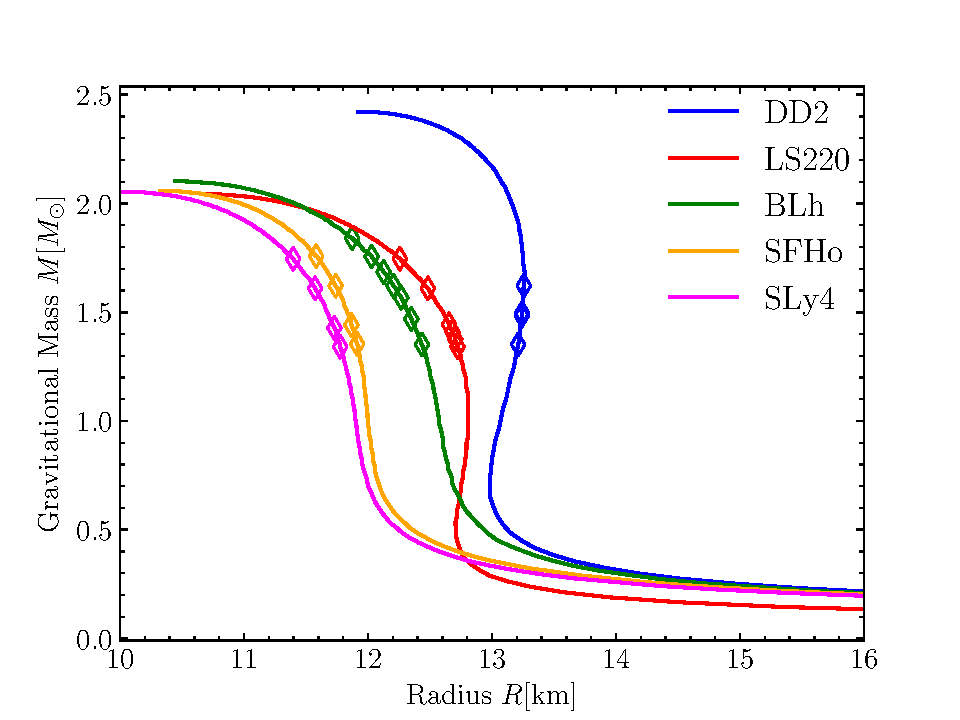
\includegraphics[width=0.49\textwidth]{./figs/tov_mr.pdf}
    \caption{Mass-radius relations for the EOSs used in this work. 
        Markers along the sequences indicate the NSs smulated in this work.}  
    \label{fig:method:tov_mr}
\end{figure}

For our models we use $5$ microphysical equation of states, namely the 
DD2 \cite{Typel:2009sy,Hempel:2009mc}, 
BLh, \red{Fill Refs}
LS220, \cite{Lattimer:1991nc}
SFHo \cite{Steiner:2012rk} and 
SLy4. \red{Refs}
.

The maximum neutron star masses and radii that these EOS predict are in line with the current astrophysical constraints, 
\textit{e.g.,} LIGO/Virgo constrain on tidal deformability 
\cite{TheLIGOScientific:2017qsa,Abbott:2018wiz,De:2018uhw,Abbott:2018exr}

Specifically, the LS220 is based on the liquid droplet Skyrme model. It has a especially steep dependency of its symmetry 
energy on density.

The DD2 and SFHo are based on nuclear statistical equilibrium.
In these EOSs a finite volume correction coupled to a relativistic mean field theory for treating high-density nuclear matte. However, between these EOSs mean-field nuclear interactions have different parameterizations and values.

To characterize these EOS, that employs very different microphyscis and finite temperature properties and their relation to the electron fraction, we consider the TOV solutions, presented on the figure \ref{fig:method:tov_mr}.
The maximum mass of a non-rotating NS that these EOSs support are $2.06$, $2.06$, $2.42$ $None$ $None$ 
for SFHo, LS220, DD2, BLh and SLy4 respectively. The NS radii, $R_{1.4}$, then $11.9$, $12.7$, $13.2$ $\red{None}$ $\red{None}$, which 
in turn is related to the pressure at half saturation density \cite{Lattimer:2012nd}. Thus we adopt the following naming convention for EOS. Those that lead to a NS with smaller radii are called "softer" and those that lead to a NS with larger radii are referred to as "stiffer" EOS.

In \red{all?.. except BLh?} EOS the finite temeperature behaviour of EOSs is largely set by the nucleon effective mass.
Then, the smaller the effective mass, the higher the temperature (assuming that entropy is unchanged).
For LS220, the nucleon mass is its bare nucleon mass (for any density) \gray{so... $m_{N}^*=m_{N}$??}.
For SFHo, $m_N ^* / m_N = 0.76$ at saturation density.
For DD2 $m_N^*/m_N = 0.56$
For BLh $\red{None}$
For SLy4 $\red{None}$
where $m_{N}^*$ is the effective nucleon mass and $m_N$ is the bare nucleon mass.



\subsection{Setup}



The simulation domain is a cube of $3.024$~km each side, whose center is at the center of mass pf the binary.
The AMR structure has $7$ refinemnt levels, with the finest convering both compact objects during the inspiral and the remnant postmerger.

We consider several resolution setups. Low resolution (LR) simulations have $h=246$~m, standard resolution (SR) 
have $h=185$~m and high resolution (HR) $h=123$~m for the final refinemnt level.

In the simulations where the neutirno M0 scheme is included, it is switched on shortly before the merger. 
The equations \eqref{eq:method:whisky:eq7} and \eqref{eq:method:whisky:eq9} are solved on the uniform spherical grid
with radius $\approx 756$~km, and resolution $n_r\times n_{\theta}\times n_{\phi} = 3096 \times 32 \times 64$
grid points.

A subset of models discussed in this thesis include the effective treatment of viscosity. 

We consider \red{$33$} distinct binary with total masses $\red{[None,None]}$ and mass-ratio $q\in[1.00,1.82]$.
In all models the neutrino leackage plus M0 scheme. Most models were computed at at least two resolutions. 
Most our models also include the effect of subgrid turbulence, viscosity.

\gray{Summary of all results in given in the table...}

\gray{Each run is nameed as}

\gray{We simulate each model for at least $\red{None}$~ms after the merger or a few milliseconds after BH formation}


 
%% ================================================================= APPENDIXES 
\appendix
%% %% ==============================================================================
%% ==============================================================================
%% ==============================================================================
%%
\part{Numerical relativity simulations of neutron star mergers}
%% \label{sec:part1}
%%
%% ==============================================================================
%% ==============================================================================
%% ==============================================================================

%% In this part to discuss
%% GR Hydro 
%% Numerical methods for GR Hydro
%% Radiation
%% M0 scheme for neutrinos
%% WhiskyTHC & Lorene
%% GW1708017 targeted models
%% Remannt/Disk dynamics of model 

%% ===========================================================================
%%
%% Theoretical Background
%%
%% ===========================================================================

\section{Basic Notations and definitions}

%% ================= | Diff.forms, external prodcuts; Hoge star | ==============
\iftoggle{Full}{
    
    \subsection{More on the tangent and cotangent spaces}
    Tangent space to $\mathcal{M}$ is denoted with $T_p(\mathcal{M})$.
    The cotangent space $T_p ^* \mathcal{M}$
    
    %% ---------------------------
    
    \subsection{Differential forms}
    \gray{copied}
    
    They are usefull for multivariable calculus independent of coordinates. Used for integrands over curves, manifolds. For example, differential form can be used to define a volume element as $f(x,y,z)dx \wedge dy \wedge dz$, where $\wedge$ is the \textit{wedge product} defined below.
    
    Albegra of differential forms is organized to reflect the orientation of the domain of integration. For instance: the \textit{exterior product} (see below) $d$ that converts $k$-from into $k+1$-form. 
    This operation is similar to the divergence and the curl of a vector field.
    
    Differential $1$-forms are naturally dual to \textit{vector fields} on a manifold. Pairing is done via \textit{inner product}.
    
    If there are two \textit{manifolds}, then the albegra of diff.forms and their exterior derivatives is preserved by the \textbf{pullblack} under the smooth function. 
    This allows geometrically invariant information to be moved from one space to another via the pullback.
    
    Let $\mathcal{M}$ be an orientated $m$-dimentional manifold and $\mathcal{M}'$ is the same manifold with the opposite orientation and $\omega$ is an $m$-form, then 
    
    \begin{equation}
    \int_{\mathcal{M}}\omega = -\int_{\mathcal{M}'}\omega.
    \end{equation}
    
    The \textit{exterior algebra} is used to make the notion of an oriented density precise.
    
    The basic $1$-forms are \textbf{differentials} of the coordiantes $dx^1,...,dx^n$. 
    Each of them is a \textbf{covector} that measures a small displacement in the corresponding coordinate direction. A general $1$-form thus is the combination of these differentials 
    \begin{equation}
    f_1dx^1\cdot\cdot\cdot f_ndx^n
    \end{equation}
    where $f_k=f_k(x^1,...,x^n)$ are functions of all the coordiantes. 
    
    \textit{Wedge product} is similar to \textit{cross product}, and is used to build higher differential forms out of lower ones, as the cross product in vector calculus.
    
    The \textit{Exterior derivative}, operator $d$ is a generalization of a differential of a function. 
    Let $\omega=fdx^I$ be a simple $k$-form. Then its exterior derivative $d\omega$ is a $(k+1)$-form set by taking differential of the coefficient functions
    \begin{equation}
    d\omega = \sum_{i=1}^n \frac{\partial f}{\partial x^i}dx^i \wedge dx^I
    \end{equation}
    Thus a \textit{deferential form}, lets say, differential $2$-form is called an exterior derivative $da$ of $a=\sum_{j=1}^{n}f_j dx^j$. 
    It is given by
    \begin{equation}
    da = \sum_{j=1}^n df_j \wedge dx^j = \sum_{i,j=1}^n \frac{\partial f_j}{\partial x^i}dx^i\wedge dx^j.
    \end{equation}
    Overall, the $da=0$ is required for a function $f$ such that $a=df$.
    
    On as smooth manifold $\mathcal{M}$ the differential from of degree $k$ is a \textit{smooth section} of the $k$th \textit{exterior power} of the \textit{cotangent bundle} of $\mathcal{M}$. 
    Then, the set of all the $k-$forms on $\mathcal{M}$ is a \textit{vector space} $\Omega^k(\mathcal{M})$. 
    The formal definition then stands. At any point $p\in \mathcal{M}$ a $k-$form $\beta$ defines an element 
    \begin{equation}
    \beta_p\in\Lambda^kT^* _p \mathcal{M}
    \end{equation}
    where $T_p\mathcal{M}$is the \textit{tangent space} tp $\mathcal{M}$ at $p$. The $T^* _p \mathcal{M}$ is its \textit{dual space} (cotangent space). Thus, $\beta$ is also a linear functional such that $\beta_p:\Lambda^k T_p \mathcal{M}\rightarrow I\!R$
    
    %% -----------------------------------------------------
    
    \subsection{More on the algebra of differential forms}
    
    If $\phi$ and $\psi$ are the 2-forms given for example as 
    \begin{equation}
    \phi = x dx - y dy \hspace{5mm} \text{and} \hspace{5mm}\psi = z dx + x dz
    \end{equation}
    Then the \textbf{exterior product} is given by 
    \begin{align}
    \phi\wedge\psi &= (x dx - y dy)\wedge(zdx + xdz) = \\
    &=xzdxdx+x^2dxdz-yzdydx-yxdydz= \\
    &=yzdxdy + x^2 dx dz - xydydz
    \end{align}
    as $dxdx=0$ and $dydx=-dxdy$. 
    The product of two $1$-forms is a $2$-form.
    In general, the \textbf{wedge product} of a $p$-form and $q$-form is a $(p+q)$-form.
    
    In other words, consider a surface $\mathcal{M}$ and two $1$-forms on it $\phi$ and $\psi$ Then the \textbf{wedge product} is 
    \begin{equation}
    (\phi\wedge\psi)(v,w)=\phi(v)\psi(w) - \phi(w)\psi(v)
    \end{equation}
    for any $v$ and $w$ tangent vectors to $\mathcal{M}$.
    
    \paragraph{Properties of the wedge product.} The exterior algebra main idea is that the operations are designed to create \textbf{the permutational antisymmetry}. 
    Let the $dx_i$ be the basis $1$-from and $\omega_j$ are the orbitrary $p$-form (of order $p_j$), and $a$, $b$ be arbitrary scalars. 
    Then the \textit{wedge product} is defined to have properties:
    \begin{align}
    (a\omega_1+b\omega_2)\wedge\omega_3 &= a\omega_1\wedge\omega_3+b\omega_2\wedge\omega_3 \hspace{5mm} (p_1 = p_2), \\
    (\omega_1\wedge\omega_2)\wedge\omega_3 &= \omega_1\wedge(\omega_2\wedge\omega_3), \hspace{5mm} a(\omega_1\wedge\omega_2) =  (a\omega_1)\wedge\omega_2\\
    dx_i\wedge dx_j &= -dx_j\wedge dx_i
    \end{align}
    Thus, any arbitrary differential form can be reduced to \textbf{a} coefficient multiplying $dx_i$ or a wedge product of the generic form 
    \begin{equation}
    dx_i\wedge dx_j \wedge...\wedge dx_p
    \end{equation}
    with the properties allowing to put all coefficients together as 
    \begin{equation}
    a dx_1 \wedge b dx_2 = - a(b dx_2 \wedge dx_1) = -ab(dx_2 \wedge dx_1) = ab(dx_1 \wedge dx_2)
    \end{equation}
    
    \paragraph{Wedge product acting on tangent vectors}.
    The $\wedge$ of two tangent vectors $\boldsymbol{u}\wedge\boldsymbol{v}$, where ($\boldsymbol{u}, \boldsymbol{v}\in T_p(\mathcal{M})$) is an antisymmetric tensor product that in addition to bilinearity requires antisymmetry. 
    \begin{align}
    \boldsymbol{v} =& v^1e_1 + v^2 e_2 + v^3 e_3 \\
    \boldsymbol{u} =& u^1e_1 + u^2 e_2 + u^3 e_3 \\
    \boldsymbol{v}\wedge\boldsymbol{u} =& (v^1u^1 - v^2u^1)(e_1\wedge e_2) + \\
    & + (v^1u^3 - v^3u^1)(e_1\wedge e_1) + \\
    & + (v^2u^3 - v^3u^2)(e_2\wedge e_1)
    \end{align}
    mimicking the behavior of the cross product. 
    However, this can easly be extended to higher dimensions. 
    
    Important, that the resulting object of $\boldsymbol{v}\wedge\boldsymbol{u}$ does not belong to $T_p M$. It is called an \textbf{alternating bivector} and is an element of the vector space $\Lambda^2 T_p (\mathcal{M})$ ,that is called -- \textbf{second exterior power} of $T_p \mathcal{M}$.
    
    Generally one obtains $\Lambda^k T_p (\mathcal{M})$ that is a linear subspace of $T_p ^k (\mathcal{M})$.
    
    Note that the exterior product on the \textit{cotangent spaces}, $T_p ^* \mathcal{M}$ is compatible with \textit{wedge product} on $T_p\mathcal{M}$ and is usually denoted with the same symbol and yields
    $(\boldsymbol{\alpha}\wedge\boldsymbol{\beta})\in\Lambda^2 T_p ^* \mathcal{M}$.
    
    %% ------------------------------------------------------
    
    \subsection{Differential forms on a Reimannian maniforld}
    
    There metric defines a fiber-wise isomorphism of the tangent and cotangent spaces. This allows to convert vector fields to covector field and vice versa. It also allows the definition of the \textit{Hodge star operator}.
    
    Hodge star operator $\star$ is a linear map, defined on the exterior algebra of a finite-dimensional oriented vector space endowed with a non-degenerate symmetric bilinear form. Applying the operator to the element of the algebra produces the \textit{Hodge dual} of the element.
    
    Example. Consider a $3D$ Euclidean space. Let there be an orientated plane, that is presented by the exterior product $\wedge$ of two basis vectors. Then its \textit{Hodge dual} is the normal vector given by the cross product. 
    
    The \textit{Hodge operator} $\star$ is a one-to-one mapping of $k-$ to $(n-k)$-vectors.
    
    The $\star$ can be applied to the \textit{cotangent bundle} of a pseudo-reimanian manifold -- to all differential $k$-forms. This allows the definition of a differential as a \textit{Hodge adjoint} of the exteior derivative. 
    
    \paragraph{Formal definition}. Let $V$ be a $n$-dimensional vector-space with non-degenerate symmetric bilinear form $\langle\cdot,\cdot\rangle$ -- the \textit{inner product}. 
    This induces an inner product on $k-$vectors $\alpha,\beta\in\Lambda^k V$ for $0\leq k \leq n$ by defining it on decomposable $k$-vectors $\alpha = \alpha_1\wedge\cdots\wedge\alpha_k$ and $\beta=\beta_1\wedge\cdots\wedge\beta_k$.
    
    The \textit{Hodge star} operator is a linear operator on the exterior algebra of $V$, mapping $k$-vectors to $(n-k)$-vectors for $0\leq k \leq n$. It has following property that defines it completely
    \begin{equation}
    \alpha\wedge(\star\beta) = \langle\alpha,\beta\rangle\omega 
    \end{equation}
    for every pair of $k-$vectors $\alpha\beta\in\Lambda^kV$.
    Here the $\omega\in\Lambda^nV$ is the unit $n-$vector defined in terms of an oriented orthonormal basis $\{e_1,...,e_n\}$ of $V$ as
    \begin{equation}
    \omega := e_1 \wedge \cdots \wedge e_n.
    \end{equation}
    
    Dually, in the space $\Lambda^n V^*$ of $n-forms$, the dual $\omega$ is the column form $\textbf{det}$, the function whose value on $v_1\wedge\cdots\wedge v_n$ is the determinant of the $n\times n$ matrix assembled from the column vectors of $v_i$ in $e_i$ coordinates. Thus the dual definition is 
    \begin{equation}
    \text{det}(\alpha\wedge\star\beta) = \langle\alpha,\beta\rangle.
    \end{equation}
    or equivalently 
    \begin{align}
    \alpha =& \alpha_1\wedge\cdots\wedge\alpha_k \\
    \beta =& \beta_1\wedge\cdots\wedge\beta_k \\
    \star\beta =& \beta_1 ^{\star} \wedge\cdots\wedge \beta_{n-k} ^ {\star} \\
    \text{det}(\alpha_1\wedge\cdots\wedge\alpha_k\wedge\beta_1 ^{\star}\wedge\cdots\wedge\beta_{n-k}^{\star}) =& \text{det}(\langle\alpha_i,\beta_j\rangle)
    \end{align}
    
    \paragraph{Examples}.
    Consider 2D space with normalized Euclidian metric and orientation given by ordering $(x,y)$. The \textit{Hodge star} on $k-$forms is given by 
    
    \begin{align}
    \star 1 &= dx \wedge dy \\
    \star dx &= dy \\
    \star dy &= -dx \\
    \star(dx \wedge dy) &= 1.
    \end{align}
    
    Consider a more complex example. A plane that can be regarded as a vector space with a standard sesquilinear form as the metric. 
    There the \textit{Hodge operator} has a property that it is invariant under the holomorphic changes of coordinates. 
    Consider $z = x + iy$ holomorphic function of $w=u + iv$. Then in the new coordinates 
    
    \begin{align}
    \alpha &= pdx +qdy \\
    \star \alpha &= -q dx + p dy
    \end{align}
    
    Next, consider a 3D space. 
    Here the $\star$ can be regarded as a correspondence between vectors and bivectors. 
    Thus in Eucledian $\boldsymbol{R}^3$ space with basis $dx,dy,dz$, of one-forms, one finds
    \begin{align}
    \star dx =& dy\wedge dz \\
    \star dy =& dz\wedge dx \\
    \star dz =& dx \wedge dy \\
    \end{align}
    The relations to the exterior and cross product are:
    \begin{equation}
    \star(\boldsymbol{u}\wedge\boldsymbol{v})=\boldsymbol{u}\times\boldsymbol{v}, \hspace{5mm}\star(\boldsymbol{u}\times\boldsymbol{v}) = \boldsymbol{u}\wedge\boldsymbol{v}
    \end{equation}
    
    Thus in 3D the $\star$ provides and isomorphism between vectors and bivectors, so each axial vector $\boldsymbol{a}$ is associated with the bivector $\boldsymbol{A}$ as $\boldsymbol{A} = \star\boldsymbol{a}$ and $\boldsymbol{a} = \star\boldsymbol{A}$. It can also mean a correspondence between the axis and infinitesimal rotation around the axis with the speed equal to the length of the axis vector.
    
    Consider a tensor $dx \otimes dy$ that corresponds to the matrix with one $dx$ row and $dy$ column. The wedge $dx\wedge dy = dx\otimes dy - dy\otimes dx$ is a 3 by 3 \textit{skew-symmetric matrix} with all $0$ exept $(0,1)$ and $(1,0)$ components that are $1$. 
    So the $\wedge$ operator turns $\boldsymbol{v} = adx + bdy + cdz$ into $\star\boldsymbol{v}\approx$ $3\times 3$ matrix with $0$ on diaoganals.
    
    Next, consider $4D$ space.
    Here $\star$ acts as an endomorphism of the second exterior power, mapping $2$-forms into $2$-forms. 
    Consider the Minkowski space time with signature $(+,-,-,-)$ and coordinates $(t,x,y,z)$, there we have
    \begin{align}
    \star dt &= dx \wedge dy \wedge dz \\
    \star dx &= dt \wedge dy \wedge dz \\
    \star dy &= -dt \wedge dx \wedge dz \\ 
    \star dz &= dt \wedge dx \wedge dy 
    \end{align}
    
    \paragraph{Wedge product on manifold}
    For an $n-$dimensional oriented pseudo-Reimannian manifold $\mathcal{M}$ we apply the construction such that to each cotangent vector space $T^* _p \mathcal{M}$ and its exterior powers $\Lambda^k T_p ^* \mathcal{M}$ and hence to all differential $k-$forms $\xi\in\Omega^k(\mathcal{M})=\Gamma(\Lambda^k T^* \mathcal{M})$, the global sections of the bundle are $\Lambda^k T^*\mathcal{M}\rightarrow \mathcal{M}$. 
    The Reimannian metric induces inner product on $\Lambda^k T_p ^* \mathcal{M}$ at each point $p\in\mathcal{M}$. We define the \textit{Hodge dual} of a $k-$form $\xi$ defining $\star\xi$ as a unique $(n-k)$-form satisfying
    \begin{equation}
    \eta\wedge\star\xi = \langle\eta,\xi\rangle\omega
    \end{equation}
    for every $k-$form $\eta$ where $\langle\eta,\xi\rangle$ is a real value function on $\mathcal{M}$ and the volume form $\omega$ is induced by the Reimannian metric.
    
    \paragraph{In the coordinate form}
    Consider an orthonormal basis $\{ \frac{\partial}{\partial x_1}, \cdots,\frac{\partial}{\partial x_n} \}$ the a tangent space $V=T_p\mathcal{M}$. And its dual basis $\{ dx_1, ..., dx_n \}$ in $V^* = T_p ^*\mathcal{M}$, with the metric matrix $g_{ij} = \big(\langle\frac{\partial}{\partial x_i},\frac{\partial}{\partial x_j}\rangle\big)$ and its inverse matrix $g^{ij} = \big(\langle dx_i, dx_j \rangle\big)$. The Hodge dual of a decomposable $k$-form is then 
    \begin{equation}
    \star(dx^{i_1}\wedge\cdots\wedge dx^{i_k}) = \frac{\sqrt{|\text{det}[g_{ab}]|}}{(n-k)!}g^{i_1 j_1}\cdots g^{i_k j_k} \epsilon_{j_1 ... j_n} dx^{j_{k+1}}\wedge\cdots\wedge dx^{j_n}
    \end{equation}
    
    %%
    
    \subsection{Conclusion}
    
    In this section we aimed to define certain mathematical concepts crucial for understanding next sections of this chapter.
    
    Particular attentions deserve the concept of tangent vectors $\partial x_i$ and cotangent vectors $\alpha_i$ that on a manifold form tangent $T_p \mathcal{M}$ and contangent $T_p^*\mathcal{M}$ spaces. The manifold that assembles all the tangent vectors is denoted with $T\mathcal{M} = \{ (x,y) | x\in \mathcal{M}, y \in T_x \mathcal{M} \}$, with the projection $\pi:T\mathcal{M}\rightarrow \mathcal{M}$, while the cotangent bundle is a smooth manifold that assembles all the cotangent spaces.
    
    The operation of importance are the \textit{inner product} $\langle \cdot,\cdot \rangle : V \times V \rightarrow \mathcal{F}$, that is linear, positive and conjugate-define, and it allows the paring between vectors and differential forms; 
    and the \textit{outer, Wedge, product} which, acting on vectors, mimics the behavior of the cross product, and acting on differential forms converts $k$-from into $k+1$-form, allowing for instance to define a volume element, $f(x,y,z)dx \wedge dy \wedge dz$. 
    
    Another important concept related to the differential forms on a Reimannian manifold is the Hodge star operator, that allows to convert vector fields into the co-vector fields and vise versa.
    
    For example, for an orientatned plane in Eqclidean space,
    the Hodge dual of the $\wedge$ product of two basis vectors is the normal vector (given by the cross product).
    
    Thus \textit{Hodge operator} $\star$ is a one-to-one mapping of $k-$ to $(n-k)$-vectors.
    
}{
    pass
}

\section{General-relativity}
%% [ GENERAL RELATIVITY from EFE to CCZ4 ]
\iftoggle{Full}{
    
    %% ---
    
    \subsection{The Cauchy Problem in General Relativity}
    
    %% ---
    
    In this section we briefly recall the initial-value formulation of the Einstein equations of general relativity through the following steps. 
    We start by introducing notations and the basics of GR. 
    We summarize the Einstein field equations. 
    Then we continue with how EFE can be split in a set of evolutionary equations and constraints. 
    For that we focus on the Arnowitt, Deser and Misner, or ADM, formalism. 
    In the end we comment on the stability of the ADM equations, on the need for strongly-hyperbolic formulations of the EFE, and on the choice of gauge conditions commonly used to evolve spacetimes with singularities. 
    This overview is based in \cite{Arnowitt:1962hi,Landau:1982dva,Wald:1984,Misner:1973,Baumgarte:2002jm}, which we refer to for more detained discussion.
    
    %% --- 
    \subsubsection{Euler-Lagrange equations}
    %% ---
    
    \red{Requires understanding of: vectors, differential forms and tensors;
        differential equation types: ellipitc, parabolic, hyperbolic, their nmerical advantages;
        smooth manifolds, Lorenzian maniforld and metric, affine connection (Levi-Civita connection), covariant derivatives, action pinciple, lagrange field theory, variation of the action, Einstein-Hilbert action, Ricci scalar and Ricci tensor, Riemann tensor;
        spacelike, timelike and null hypersurface, hyperbolic space-time, space-time foliation,
        Lie-derivative along the vector field, Lagrangian density, Legendre transformation, Hamiltonian,
        extrinsic curvature, Codazzi equations, Gauss equations,
        palantini-type vatiation
        gauge conditions: slicing and spatial,}
    
    We consider a spacetime defined by the real \textit{smooth manifold} $\mathcal{M}$ and \textit{Lorentzian metric} $\boldsymbol{g}$ on $\mathcal{M}$ of signature $(-,+,+,+)$. 
    The $\nabla$ denotes the \textit{affine connection} associated with $\boldsymbol{g}$, the Levi-Civita connection.
    We use the convention that all Greek indices lie in $\{0, 1, 2, 3\}$ and Lower case Latin indices $\{1, 2, 3\}$.
    The $\nabla\boldsymbol{T}$ denotes the \textit{covariant derivative} of a tensor $\boldsymbol{T}$ and $\nabla_{\boldsymbol{u}}\boldsymbol{T}$ -- covariant derivative along a given vector field $\boldsymbol{u}$.
    
    The scalar product of two vectors then 
    
    \begin{equation}
    \boldsymbol{a}\cdot\boldsymbol{b}:=g_{\mu\nu}a^{\mu}b^{\nu}
    \end{equation}
    
    The action of a linear form on a vector however is represented as 
    
    \begin{equation}
    \langle\boldsymbol{\omega},\boldsymbol{\upsilon}\rangle=\omega_{\mu}\upsilon^{\mu}
    \end{equation}
    
    Let the $\boldsymbol{\alpha}$ be the \textit{totally antisymmetric symbol} that expresses through coordinates $x^{\mu}$ as
    
    \begin{equation}
    \boldsymbol{\alpha} = dx^0 \wedge dx^1 \wedge dx^2 \wedge dx^3,
    \end{equation}
    
    where $\wedge$ denotes \textit{exterior product}. 
    Then, proper \textit{volume pseudo-form} of the spacetime is
    
    \begin{equation}
    \boldsymbol{\varepsilon} = \sqrt{-g}\boldsymbol{\alpha},
    \end{equation}
    
    where $g$ denotes the determinant of the spacetime metric.
    
    In GR, the spacetime is represented by \textit{Lorentzian manifold} $\mathcal{M}$ and $g$, the \textit{Lorentzian metric}.
    
    The \textit{action principle} of the \textit{Lagrangian field theory} on the spacetime $(\mathcal{M}; \boldsymbol{g})$ is
    
    \begin{equation}
    S(\boldsymbol{q}, \nabla\boldsymbol{q}) = \int_{\mathcal{M}}\boldsymbol{\alpha}\mathcal{L}(\boldsymbol{q}, \nabla\boldsymbol{q}),
    \end{equation}
    
    where $\boldsymbol{q}$ are a set of generalized coordinates for the fields described by the theory, $\nabla$ is the Levi-Civita connection, $\mathcal{L}$ is a scalar density of a scalar quantity $\lambda$ as $\lambda(\boldsymbol{q},\nabla\boldsymbol{q})$. 
    
    Varying the action with respect to the $\boldsymbol{q}$
    
    \begin{equation}
    \delta S(\boldsymbol{q}, \nabla\boldsymbol{q}) = \delta\int\boldsymbol{\alpha}\mathcal{L}(\boldsymbol{q}, \nabla\boldsymbol{q}) = \int\boldsymbol{\alpha}\Big(\frac{\partial\mathcal{L}}{\partial\boldsymbol{q}}\delta\boldsymbol{q}+\frac{\partial\mathcal{L}}{\partial(\nabla\boldsymbol{q})}\delta\nabla\boldsymbol{q}\Big)
    \end{equation}
    
    As $\delta$ and $\nabla$ commute, and partially integrating $\nabla$, we obtain
    
    \begin{equation}
    \partial S(\boldsymbol{q}, \nabla\boldsymbol{q}) = \int\boldsymbol{\alpha}\Big(\frac{\mathcal{L}}{\partial\boldsymbol{q}}-\nabla\frac{\partial \mathcal{L}}{\partial(\nabla\boldsymbol{q})}\Big)\delta\boldsymbol{q} + \int_{\mathcal{M}}\boldsymbol{\alpha}\nabla\Big(\frac{\partial\mathcal{L}}{\partial(\nabla\boldsymbol{q})}\delta\boldsymbol{q}\Big)
    \end{equation}
    
    The last term is a boundary term and in order to vanish we impose boundary condition. 
    Assume that the fields are defined over only a \textit{compact domain}. \\
    As the choice of $\partial\boldsymbol{q}$ is arbitrary, the 
    
    \begin{equation}
    \partial S(\boldsymbol{q}, \nabla\boldsymbol{q}) = 0
    \end{equation}
    
    and the \textit{Euler-Lagrange equations} are
    
    \begin{equation}
    \frac{\partial \mathcal{L}}{\partial\boldsymbol{q}} - \nabla\Big(\frac{\partial\mathcal{L}}{\partial(\nabla\boldsymbol{q})}\Big) = 0
    \label{eq:theory:eulerlagrange}
    \end{equation}
    
    %% ---
    \subsubsection{The Hilbert Action}
    %% ---
    
    The \textit{Einstein-Hilbert action} allows to obtain an \textit{Einstein field equations} through the \textit{principle of least action}. Here we briefly underline the procedure.
    
    Introduce action that describes the gravitational field, and a matter field $\mathcal{L}_m$:
    
    \begin{align}
    S_g &= \int\frac{1}{2\kappa}R\epsilon, \\
    S_m &= \int\mathcal{L}_{m}\epsilon,
    \end{align}
    
    where $R$ is the Ricci scalar and $\kappa$ is the  Einstein's constant.
    
    The full action then:
    
    \begin{equation}
    S = \int\Big(\frac{1}{2\kappa}R+\mathcal{L}_m\Big)\epsilon
    \end{equation}
    
    The action principle dicatates, that $\delta S = 0$  with respect to the inverse metric $g^{\mu\nu}$. 
    
    \begin{equation}
    \int\Bigg[\frac{1}{2\kappa}\Big(\frac{\delta R}{\delta g^{\mu\nu}}+\frac{R}{\sqrt{-g}}\frac{\delta\sqrt{-g}}{\delta g^{\mu\nu}}\Big) + \frac{1}{\sqrt{-g}}\frac{\delta(\sqrt{-g}\mathcal{L}_m)}{\delta g^{\mu\nu}}\Bigg]\delta g^{\mu\nu}\epsilon
    \end{equation}
    
    Owing to the arbitrariness of $\delta g^{\mu\nu}$, the integrand must be zero. 
    
    \begin{equation}
    \frac{\delta R}{\delta g^{\mu\nu}} + \frac{R}{\sqrt{-g}}\frac{\delta\sqrt{-g}}{\delta g^{\mu\nu}} = -2\kappa\frac{1}{\sqrt{-g}}\frac{\delta(\sqrt{-g}\mathcal{L}_m)}{\delta g^{\mu\nu}} = -\frac{2\kappa}{\sqrt{-g}}\frac{\delta S_m}{\delta g_{\mu\nu}} := \kappa T_{\mu\nu},
    \label{eq:theory:action1}
    \end{equation}
    
    where we introduced the stress-energy tensor $T_{\mu\nu}$ and the matter action $S_m$ for future use. \\
    
    \gray{this matter action is used in deriving the $T_{\mu} ^{\nu}$ i the invariant fluid formalism}
    
    The continuation of this derivation requires taking variation of the Riccia scalar $R$ and the determinant of the metric $\sqrt{-g}$. 
    As this is a length procedure, we provide here the result. 
    
    \begin{equation}
    \frac{\delta R}{\delta g^{\mu\nu}} = R_{\mu\nu},
    \label{eq:theory:deltaR}
    \end{equation}
    
    where the $R_{\mu\nu}$ is the Ricci curvature tensor.
    
    \begin{equation}
    \frac{1}{\sqrt{-g}}\frac{\delta\sqrt{-g}}{\delta g^{\mu\nu}} = -\frac{1}{2}g_{\mu\nu}.
    \label{eq:theory:deltagmuny}
    \end{equation}
    
    Substituting Eq. \ref{eq:theory:deltaR} and Eq. \ref{eq:theory:deltagmuny} into equation of motion Eq.  \ref{eq:theory:action1} we obtain the Einstein's field equation 
    
    \begin{equation}
    R_{\mu\nu} -\frac{1}{2}g_{\mu\nu}R=8\pi T_{\mu\nu},
    \label{eq:theory:EFE}
    \end{equation}
    
    where in the geometrized unit system, \textit{i.e} $c=G=1$, the $\kappa=8\pi$.
    
    %% ---
    \subsubsection{3+1 Decomposition of Einstein field equations}
    %% ---
    
    The Einstein field equations (\ref{eq:theory:EFE}) represent a set of $10$ non-linear partial differential equations.
    These equations can be defined on a while metric $\mathcal{M}$ or a domain $\Omega\subset\mathcal{M}$, where in the latter, the boundary conditions on $\partial\Omega$ are required. 
    
    It is convenient to chose a \textit{null hyersurface} $\Sigma\subset\mathcal{M}$ on which to define the initial data, from which the evolution of space-time begins. 
    This, however, requires the spacetime to be \textit{strongly hyperbolic}, meaning that the foliation $\mathcal{M}=\Sigma\times\mathbb{R}$ is allowed. 
    This foliation can be understood as splitting the spacetime into a set of \textit{spacelike} hypersurfaces $\Sigma_t$. 
    
    
    \paragraph{Spacelike Foliations}
    
    
    Let the $t$ be the global smooth functions such that, 
    
    \begin{equation}
    \Sigma_{\tau} = \{x^{\alpha}\in\mathcal{M}: t(x^{\alpha})=\tau\},
    \end{equation}
    
    and let $\vec{t}$ be a vector such that $\langle\nabla t, \vec{t}\rangle = 1$. 
    This $t$ can be seen as a "function that advances time" and $\vec{t}$ as a "flow of time" vector field.
    Continuing the analogy, the rate at which a given tensor quantity $\boldsymbol{q}$ changes between hypersurfaces $\Sigma_t$ is given by the \textit{Lie derivative} of the $\boldsymbol{q}$ along the vector $\vec{t}$.
    
    Consider two hypersurfaces $\Sigma_t$ and $\Sigma_{t+dt}$. 
    A transition from one to another can be decomposed into the part tangent to the hypersurface $\Sigma_{t+dt}$ and expressed in a form of a vector $\vec{\beta}$ and a pert normal to the hypersurface $\Sigma_t$ and expressed as a $\alpha \vec{n}$, where $\vec{n}$ is a unit vector, normal to the $\Sigma_t$ in the diretion to $\Sigma_{t+dt}$. 
    Then, the vector $\vec{t}$ can be written as 
    
    \begin{equation}
    \vec{t} = \alpha\vec{n}+\vec{\beta}.
    \end{equation}
    
    $\vec{\beta}$ is called \textit{shift vector} and $\alpha$ is called \textit{lapse-function}. 
    
    The spacetime metric $\boldsymbol{g}$ can be decomposed into a spatial, \textit{Riemannian metric} $\boldsymbol{\gamma}$ as $\boldsymbol{\gamma} = \boldsymbol{g} + \underline{n} \otimes \underline{n}$, where $\underline{n}$ is the 1-form associated to the vector $\vec{n}$. \red{and?}
    The \textit{Levi-Civita connection} can be computed by projecting the $\nabla$ on the space, tangent to the hypersurface $\Sigma_t$.
    
    There are exist coordinates that are adapted to the foliation, namely $\{t, x^i\}$ with $\vec{\partial}_i\cdot \vec{n} = 0$. 
    In these coordiantes the $\nabla t = dt$ and $\vec{t} = \vec{\partial}_t$. 
    
    The connection between $\boldsymbol{g}$ and $\boldsymbol{\gamma}$ is $g_{\mu\nu}=\vec{\partial}_{\mu}\cdot\vec{\partial}_{\nu} $ and can be expressed in terms of $\alpha$ and $\vec{\beta}$ as
    
    \begin{align}
    \text{spatial components: } g_{ik}&=\vec{\partial}_{i}\cdot\vec{\partial}_{j} =\gamma_{ik}, \\
    \text{time component: } g_{tt} &= \vec{\partial}_{t}\cdot\vec{\partial}_{t} = \vec{t}\cdot\vec{t} = - (\alpha^2-\vec{\beta}\cdot\vec{\beta}), \\
    \text{mixed components: } g_{ti} &= \vec{\partial}_{t}\cdot\vec{\partial}_{i} = \vec{t}\cdot\vec{\partial}_i = (\alpha\vec{n}+\vec{\beta})\cdot\vec{\partial}_i=\beta_i,
    \end{align}
    
    where we made use of $\vec{\beta}$ being the spatial vector, \textit{i.e} $\vec{\beta}\cdot\vec{\beta}=\gamma_{ik}\beta^i\beta^k$.
    
    The line-element can be thus written as
    \begin{equation}
    ds^2 = -(\alpha^2-\beta_i\beta^i)dt^2 +2\beta_i dx^i dt + \gamma_{ik} dx^i dx^k.
    \end{equation}
    
    
    \paragraph{Ex-curse: Hamiltonian Field Theory}
    
    
    First we recall the generalized coordinates $\boldsymbol{q}$ and their \textit{covariant derivatives} $\nabla\boldsymbol{q}$. 
    
    In light of the spacetime decomposition discussed above, we divide the $\boldsymbol{\alpha}$ into the time $dt$ and spatial parts represented by the \textit{antisymmetric symbol} ${^{(3)}\boldsymbol{\alpha}}$ as 
    
    \begin{equation}
    \boldsymbol{\alpha} = dx^0 \wedge dx^1 \wedge dx^2 \wedge dx^3 = dt \wedge {^{(3)}\boldsymbol{\alpha}}.
    \end{equation}
    
    Next, we introduce the "time derivative" as a \textit{Lie derivative along the vector field} $\vec{t}$ as 
    
    \begin{equation}
    \dot{\boldsymbol{q}} := \mathcal{L}_{\vec{t}}\boldsymbol{q}.
    \end{equation}
    
    As the $\Lambda(\boldsymbol{q}, \nabla\boldsymbol{q})$ is the \textit{Lagrangian density}, a conjugate momentum can be defined as 
    
    \begin{equation}
    \boldsymbol{p} := \frac{\partial\Lambda}{\partial\dot{\boldsymbol{q}}},
    \end{equation}
    
    Assuming that $\boldsymbol{p}$ and $\nabla\boldsymbol{q}$ can be expressed as a function of $\boldsymbol{q}$ and $\boldsymbol{p}$, inspired by the \textit{Legendre transformation}, we define the \textit{Hamiltonian} and its density as
    
    \begin{align}
    \mathcal{H} &= \boldsymbol{p}\cdot\dot{\boldsymbol{q}} - \mathcal{L}(\boldsymbol{q}, \nabla\boldsymbol{q}) \\
    H &= \int_{\Sigma}\mathcal{H}{^{(3)}\boldsymbol{\alpha}}
    \end{align}
    
    Additionally we define the quantity 
    
    \begin{equation}
    J = \int_{0}^{t}H(\boldsymbol{q},\boldsymbol{p})dt = \int_{0}^{t}dt\int_{\Sigma}\mathcal{H}(\boldsymbol{q},\boldsymbol{p}){^{(3)}\boldsymbol{\alpha}} = \int_{0}^{t}dt\int_{\Sigma}{^{(3)}\boldsymbol{\alpha}}\Big(\boldsymbol{p}\cdot\dot{\boldsymbol{q}} - \mathcal{L}(\boldsymbol{q},\nabla\boldsymbol{q})\Big).
    \end{equation}
    
    Consider the variation of the $J$ with respect to the $\delta\boldsymbol{p}$ and $\delta\boldsymbol{q}$ as
    
    \begin{equation}
    \delta J = \int_{0}^{t}\delta H(\boldsymbol{q},\boldsymbol{p})dt = \int_{0}^{t}dt (\dot{\boldsymbol{q}}\delta\boldsymbol{p}+\boldsymbol{p}\delta\dot{\boldsymbol{q}}) - \int_{0}^{t}dt\delta\Lambda(\boldsymbol{q}, \nabla\boldsymbol{q}).
    \end{equation}
    
    Consider the last term. The variation of the Lagrangian is
    
    \begin{equation}
    \delta\Lambda = \int_{\Sigma}{^{(3)}\boldsymbol{\alpha}}\Bigg[\frac{\delta\Lambda}{\delta\dot{\boldsymbol{q}}}\delta\dot{\boldsymbol{q}}+\frac{\delta\Lambda}{\delta\boldsymbol{q}}\delta\boldsymbol{q}\Bigg],
    \end{equation}
    
    The first term in the square brackets can be reduced to $\boldsymbol{p}\delta\dot{\boldsymbol{q}}$, using the definition of the conjugate momentum. 
    The second term can be treated, applying the Euler-Lagrange equations (\ref{eq:theory:eulerlagrange}). 
    These manipulations result in
    
    \begin{equation}
    \delta\Lambda = \int_{0}^{t}dt\int_{\Sigma}{^{(3)}\boldsymbol{\alpha}}(\boldsymbol{p}\delta\dot{\boldsymbol{q}} + \dot{\boldsymbol{p}}\delta\boldsymbol{q}).
    \end{equation}
    
    Thus we obtain that 
    
    \begin{equation}
    \int_{0}^{t} \delta H(\boldsymbol{q},\boldsymbol{p})dt =   \int_{0}^{t}dt\int_{\Sigma}{^{(3)}\boldsymbol{\alpha}}(\dot{\boldsymbol{q}}\cdot\delta\boldsymbol{p}-\dot{\boldsymbol{p}}\cdot\delta\boldsymbol{q}),
    \end{equation}
    
    and as $\delta\boldsymbol{p}$ and $\delta\boldsymbol{p}$ are arbitrary, the \textit{Hamilton equations} read
    
    \begin{equation}
    \dot{\boldsymbol{q}}=\frac{\delta H}{\delta\boldsymbol{p}}, \hspace{5mm} \dot{\boldsymbol{p}} = -\frac{\delta H}{\delta\boldsymbol{q}}.
    \label{eq:theory:hamiltoneqs}
    \end{equation}
    
    The Hamiltonian formalism can be used to re-derive the field-equations in a from that once the initial data is specified on a hypersurface $\Sigma_0$ for $\boldsymbol{q}$ and $\boldsymbol{p}$, the equations (\ref{eq:theory:hamiltoneqs}) would govern whole the evolution.
    
    
    \paragraph{Extrinsic Curvature and Constraint equations}
    
    
    We define the \textit{extrinsic curvature} of a $D-1$-surface $\Sigma_t\subset\mathcal{M}$ at a point $\mathcal{P}\in\Sigma_t$ as mapping $\boldsymbol{K}$ such that $\boldsymbol{K}(\boldsymbol{\upsilon})=-\nabla_{\boldsymbol{\upsilon}}\boldsymbol{n}$. 
    Note, that the $\boldsymbol{K}$ does not depend on $\alpha$ and $\vec{\beta}$, it is a purely spatial tensor. 
    The components of the extrinsic curvature are 
    
    \begin{equation}
    K_{\mu\nu} = -{\gamma^{\alpha}}_{\mu}\nabla_{\boldsymbol{u}}^{\alpha} n_{\nu} = -\frac{1}{2}\mathcal{L}_{\vec{n}}\gamma_{\mu\nu},
    \label{eq:theory:extrcurvdef}
    \end{equation}
    
    where $\mathcal{L}_{\vec{n}}$ is the Lie derivative along the vector field $\vec{n}$. \\
    From the (\ref{eq:theory:extrcurvdef}) the extrinsic curvature can be interpreted as a "speed of the $\vec{n}$ during the parallel transport along the hypersurface $\Sigma_t$".
    
    \textit{Codazzi equations} relate the $4D$ Ricci tensor to the extrinsic curvature as
    
    \begin{equation}
    D_{\beta}K-D_{\alpha}{K^{\alpha}}_{\beta}=R_{\gamma\delta}n^{\delta}{\gamma^{\gamma}}_{\beta},
    \label{eq:theory:formomentum}
    \end{equation}
    
    here $K$ is a trace of the tensor $\boldsymbol{K}$.
    
    Gauss equation relates the $3D$ \textit{Riemann tensor} $^3{R_{\alpha\beta\gamma}}^{\delta}$ to the $4D$ one and the $\boldsymbol{K}$ as 
    
    \begin{equation}
    ^3{R_{\alpha\beta\gamma}}^{\delta} = {\gamma^{\mu}}_{\alpha}{\gamma^{\nu}}_{\beta}{\gamma^{\lambda}}_{\gamma}{\gamma^{\delta}}_{\sigma}{R_{\mu\nu\lambda}}^{\delta}-K_{\alpha\gamma}{K_{\beta}}^{\delta}+K_{\beta\gamma}{K^{\delta}}_{\alpha}.
    \label{eq:theory:forhamiltconst}
    \end{equation}
    
    The \textit{momentum constraint} thus can be obtained by substituting the (\ref{eq:theory:EFE}) into  (\ref{eq:theory:formomentum}) which yields
    
    \begin{equation}
    D_{\beta}K-D_{\alpha}{K^{\alpha}}_{\beta} = -8\pi{\gamma^{\alpha}}_{\beta} n^{\gamma}T_{\alpha\gamma}=:8\pi j_{\beta},
    \label{eq:theory:momconstraint}
    \end{equation}
    
    where $j^{\alpha}$ is the ADM momentum density.
    
    The \textit{Hamiltonian constraint} can be obtained by substituting EFE (\ref{eq:theory:EFE}) into the (\ref{eq:theory:forhamiltconst}), yielding 
    
    \begin{equation}
    ^3 R+ K^2 - K_{\alpha\beta}K^{\alpha\beta} = 2G^{\alpha\beta}n_{\alpha}n_{\beta} = 16\pi n_{\alpha}n_{\beta} T^{\alpha\beta} =: 16\pi E,
    \label{eq:theory:hamilconstraint}
    \end{equation}
    
    where $E$ is the ADM energy density.
    
    The obtained constraint equations represent a set of \textit{elliptic equations} that must be satisfied on every hyprsurface $\Sigma_i$ of the foliation. 
    It is however, possible to show that Einstein equations preserve the constraints, meaning that if they are satisfied at the initial slice $\Sigma_0$ they will be satisfied at any time in the future.
    
    
    \paragraph{The Hamiltonian Formulation of the Einstein Equations, ADM equations}
    
    
    \gray{deriving the evolution equations, ADM formulation}
    
    %% Part 1 [Extrinsic curvature]
    
    Here we briefly sketch to path of derivation of the Einstein field equations in the Hamiltonian framework. We will elude most of the intimidate and computationally extensive steps, as well as derivation of the boundary terms. For this we refer to \cite{Poisson:2004}.
    
    First it is useful to note that determinant of the three-metric $\sqrt{\gamma}$ can be expressed as $\sqrt{\gamma}=\sqrt{-g}/\alpha$. 
    The $p$ is the trace of the canonical momentum $\boldsymbol{p}$.
    
    Now, consider the \textit{scalar curvature}, $R$,
    
    \begin{align}
    G_{\mu\nu} &= R_{\mu\nu} - \frac{1}{2}Rg_{\mu\nu} \\
    -Rg_{\mu\nu}n^{\nu}n^{\mu} &= 2(G_{\mu\nu} n^{\nu}n^{\mu}-R_{\mu\nu}n^{\mu}n^{\mu})\\
    -Rn_{\mu}n^{\mu}& = 2(G_{\mu\nu}n^{\nu}n^{\mu} - R_{\mu\nu}n^{\mu}n^{\mu}) \\
    R &= 2(G_{\mu\nu}n^{\mu}n^{\nu} - R_{\mu\nu}n^{\mu}n^{\nu}).
    \end{align}
    
    From the \textit{Gauss-Codacci equation} (\ref{eq:theory:momconstraint}), which relates the spatial curvature $^{(3)}R$ to the spacetime curvature $R$, we have the following constraint relationship
    
    \begin{equation}
    2G_{\mu\nu}n^{\mu}n^{\nu} = {^{(3)}R} + K^2 - K_{\mu\nu}K^{\mu\nu}.
    \end{equation}
    
    The $R_{\mu\nu}n^{\mu}n^{\nu})$ can be expressed as a combination of extrinsic curvature and total divergences as follows.
    From the definition of the Ricci tensor $R_{\mu\nu}$, we have:
    
    \begin{align}
    R_{\mu\nu} &= {R_{\mu\gamma\nu}}^{\gamma} \\
    R_{\mu\nu}n^{\mu}n^{\nu} &= {R_{\mu\gamma\nu}}^{\gamma} \\
    &= -(\nabla_{\mu}\nabla_{\gamma} - \nabla_{\gamma}\nabla_{\mu})n^{\gamma}n^{\nu} \\
    &= n^{\mu}(\nabla_{\mu}\nabla_{\gamma} - \nabla_{\gamma}\nabla_{\nu})n^{\gamma} \\
    &= (\nabla_{\mu}n^{\mu})(\nabla_{\gamma}n^{\gamma}) - \nabla_{\mu}(n^{\mu}\nabla_{\gamma}n^{\gamma}) - (\nabla_{\gamma}n^{\mu})(\nabla_{\mu}n^{\gamma}) + \nabla_{\gamma}(n^{\mu}\nabla_{\mu}n^{\gamma}) \\
    &= K^2 - K_{\mu\gamma}K^{\mu\gamma} - \nabla_{\mu}(n^{\mu}\nabla_{\gamma}n^{\gamma}) + \nabla_{\gamma}(n^{\mu}\nabla_{\mu}n^{\gamma})
    \end{align}
    
    In case of variations with compact support, that we are interested in, the total divergences -- last two terms -- can be neglected. 
    Then the result is
    
    \begin{equation}
    R_{\mu\nu}n^{\mu}n^{\nu}= K^2 - K_{\mu\nu}K^{\mu\nu}.
    \label{eq:theory:rmunu_as_func_k}
    \end{equation}
    
    %% part 2 [Canonical momentum and Hamiltonian]
    
    Using the fact that $\sqrt{\gamma}=\sqrt{-g}/\alpha$ and the (\ref{eq:theory:rmunu_as_func_k}) we obtain the Lagrangian density in terms of the variables on the hypersurface:
    
    \begin{align}
    \Lambda &= \sqrt{-g}R \\
    &= \alpha\sqrt{\gamma}R \\
    &= 2\alpha\sqrt{\gamma}(G_{\mu\nu}n^{\mu}n^{\nu} - R_{\mu\nu}n^{\mu}n^{\nu})\\ 
    &= 2\alpha\sqrt{\gamma}\Big(\frac{1}{2}[{^{(3)}R} - K_{\mu\nu}K^{\mu\nu} + K^2] - K^2 - K_{\mu\nu}K^{\mu\nu}\Big)
    \end{align}
    
    Together with the contribution from matter fields, we obtain
    
    \begin{equation}
    \Lambda = \Lambda_g+\Lambda_m= \frac{1}{16\pi}\alpha({^{(3)}R} + K_{\mu\nu}K^{\mu\nu} - K^2)\sqrt{\gamma}+\Lambda_m
    \end{equation}
    
    Next we note that the extrinsic curvature of a
    surface $\Sigma$ is defined as $K_{\mu\nu} = \nabla_{\mu}n_{\nu}$. 
    
    To relate $K_{\mu\nu}$ to the metric, we make use of the following property of Lie derivatives:
    
    \begin{align}
    \mathcal{L}_{\vec{n}}g_{\mu\nu} &= n^{\gamma}\nabla_{\gamma}g_{\mu\nu} + g_{\gamma\nu}\nabla_{\mu}\upsilon^{\gamma} + g_{\mu\gamma}\nabla_{\nu}\upsilon^{\gamma} \\
    &= \nabla_{\mu}n_{\nu}+\nabla_{\nu}\upsilon_{\nu} \\
    &=2\nabla_{\mu}n_{\nu}
    \end{align}
    
    where the second line holds when $\nabla_{\gamma}\mu$ is the natural derivative operator corresponding to the metric $g_{\mu\nu}$ and the third line holds because $K_{\mu\nu}$ is symmetric.
    
    Substituting this into our definition of $K_{\mu\nu}$,
    
    \begin{align}
    K_{\mu\nu} &= -\frac{1}{2}\mathcal{L}_{\vec{\vec{n}}}g_{\mu\nu} \\
    &= -\frac{1}{2}\mathcal{L}_{\vec{\vec{n}}}(\gamma_{\mu\nu}-n_{\mu}n_{\nu}) \\
    &= -\frac{1}{2}\mathcal{L}_{\vec{\vec{n}}}\gamma_{\mu\nu} \\
    &= -\frac{1}{2}[n^{\gamma}\nabla_{\gamma}\gamma_{\mu\nu} + \gamma_{\gamma\nu}\nabla_{\mu}\upsilon^{\nu} + h_{\mu\gamma}\nabla_{\nu}\upsilon^{\gamma}] \\
    &= -\frac{1}{2\alpha}[\alpha n^{\gamma}\nabla_{\gamma}\gamma_{\mu\nu} + \gamma_{\gamma\nu}\nabla_{\mu}\alpha\upsilon^{\nu} + h_{\mu\gamma}\nabla_{\nu}\alpha\upsilon^{\gamma}] \\
    &= -\frac{1}{2\alpha}{\gamma_{\mu}}^{\gamma}{\gamma_{\nu}}^{\delta}[\mathcal{L}_{\vec{t}}\gamma_{\gamma\delta}-\mathcal{L}_{\vec{\beta}}\gamma_{\gamma\delta}] \\
    &= -\frac{1}{2\alpha}{\gamma_{\mu}}^{\gamma}{\gamma_{\nu}}^{\delta}[\partial_t\gamma_{\mu\nu}-D_{\mu}\beta_{\nu}-D_{\nu}\beta_{\mu}]
    \end{align}
    
    and on the hypersurface $\Sigma$ the \textit{projection operators} are not needed. So we obtain
    
    \begin{equation}
    K_{\mu\nu} = -\frac{1}{2}\mathcal{L}_{\vec{n}}\gamma_{\mu\nu}=-\frac{1}{2\alpha}(\partial_t\gamma_{\mu\nu}-D_{\mu}\beta_{\nu}-D_{\nu}\beta_{\mu})
    \end{equation}
    
    which allows us to express the canonical momentum $p^{\mu\nu}$ as
    
    \begin{align}
    p^{\mu\nu} &= \frac{\partial\Lambda}{\partial\dot{\gamma}_{\mu\nu}} \\
    &= -\frac{\sqrt{\gamma}}{16\pi}\alpha\Bigg[\frac{\partial {^{(3)}R}}{\partial\dot{\gamma}_{\mu\nu}} + \frac{\partial(K_{\mu\nu}K^{\mu\nu})}{\partial\dot{\gamma}_{\mu\nu}} - \frac{\partial K^2}{\partial\dot{\gamma}_{\mu\nu}}\Bigg] \\
    &= \frac{\sqrt{\gamma}}{16\pi}(K\gamma^{\mu\nu} - K^{\mu\nu}),
    \end{align}
    
    where 
    
    \begin{equation}
    \frac{\partial K_{\mu\nu}}{\partial \dot{\gamma}_{\mu\nu}} = \frac{1}{2\alpha}, \hspace{5mm} \frac{\partial {^{(3)}R}}{\partial \dot{\gamma}_{\mu\nu}} = 0, \hspace{5mm}\frac{\partial K^2}{\partial \dot{\gamma}_{\mu\nu}} = \frac{\gamma^{\mu\nu}K}{\alpha}
    \end{equation}
    
    assuming that there is no explicit dependency of the $\Lambda$ on $dot{\gamma}_{\mu\nu}$.
    
    Since, $\alpha$ and $\vec{\beta}$ are related to the the \textit{gauge freedom}, -- there are many ways the manifold $\mathcal{M}$ can be split into hypersurfaces -- the momenta associated with these functions and vectors is zero.
    
    Thus, the \textit{Hamiltonian density} is
    
    \begin{align}
    \mathcal{H} &= p^{\mu\nu}\dot{\gamma}_{\mu\nu} - \Lambda \\
    &= -\sqrt{\gamma}\alpha{^{(3)}R} + \frac{\alpha}{\sqrt{\gamma}}\Big[p^{\mu\nu}p_{\mu\nu}-\frac{1}{2}p^2\Big] + 2p^{\mu\nu} D_{\mu}\beta_{\mu} -\Lambda_m \\
    %    &=  \frac{\sqrt{\gamma}}{16\pi}\Bigg\{\alpha\Big[-{^{(3)}R}+h^{-1}p^{\mu\nu}p_{\mu\nu}-\frac{1}{2}h^{-1}p^2\Big] - 2\beta_{\nu}\big[D_{\mu}(h^{-1/2}p^{\mu\nu})\big] + D_{\mu}(h^{-1/2}\beta_{\nu}p^{\mu\nu})\Bigg\} \\
    &= \frac{\sqrt{\gamma}}{16\pi}\Bigg\{\alpha\Big[ -{^{(3)}R} + \gamma^{-1}p^{\mu\nu}p_{\mu\nu}-\frac{1}{2}\gamma^{-1}p^2\Big] +  2\beta_{\nu}\Big[D_{\mu}(\gamma^{-1/2}p^{\mu\nu})\Big] - 2D_{\mu}(\gamma^{-1/2}\beta_{\nu}p^{\mu\nu}) \Bigg\} - \Lambda_m,
    \end{align}
    
    where we restored the correct $16\pi$ factor in the last line.
    
    As we consider variations with compact suppot, the last boundary term, can be neglected.
    
    %% part 3 [Arriving at constraint equations (again)]
    
    Now we consider the variation of the matter action $S_m$ with respect to the $\alpha$ and $\vec{\beta}$
    
    \begin{align}
    \frac{\delta S_m}{\delta \alpha} &=-\alpha\frac{\delta S_m}{\delta g_{00}} = -\alpha\sqrt{-g}T^{00} = -\alpha^2\sqrt{\gamma}T^{00} = -\sqrt{\gamma}T^{\mu\nu}n_{\mu}n_{\nu} \\
    \frac{\delta S_m}{\delta \beta_{\mu}} &= \frac{\delta S_m}{\delta g_{\mu 0}} =\frac{1}{2}\sqrt{-g}T^{\mu 0} = -\frac{1}{2} \sqrt{\gamma}T^{\mu\nu}n_{\nu}.
    \end{align}
    
    As the variation of the Hamiltonian $H$ with respect to a quantity with vanishing canonical momentum is zero, we obtain two equations 
    
    \begin{align}
    \frac{\delta H}{\delta \alpha} &= 0 = -{^{(3)}R} + \gamma^{-1}p^{\mu\nu}p_{\mu\nu}-\frac{1}{2}\gamma^{-1}p^2 + 16\pi T^{\mu\nu}n_{\mu}n_{\nu} \\
    \frac{\delta H}{\delta \beta_{\mu}} &= 0 = - D_{\mu}(\gamma^{-1/2}p^{\mu\nu}) + 8\pi{\gamma^{\mu}}_{\nu}n_{\gamma}T^{\nu\gamma}.
    \label{eq:theory:hamiltonianvariation}
    \end{align}
    
    Note, that the $\delta H / \delta\beta_{\mu}$ is actually a \textit{Frech\'et differential} $dH$, $\delta \beta_{\mu}$, which is writes as
    
    \begin{equation}
    \langle dH,\delta\beta \rangle = \delta\beta_{\mu}\big[-D_{\nu}(\gamma^{-1/2}p^{\mu\nu})+8\pi n_{\gamma}T^{\mu\nu}\big], 
    \end{equation}
    
    containing $\delta\beta_{\mu}$ which is spatial. 
    
    Thus only the spatial part is being constrained in the equation above. 
    To account for that the projector ${\gamma^{\mu}}_{\nu}$ is added to the $\delta H/\delta \beta_{\mu}$.
    
    The pair of equations (\ref{eq:theory:hamiltonianvariation}) is in fact the constraint equations derived before, namely the (\ref{eq:theory:momconstraint}) and (\ref{eq:theory:hamilconstraint}), and as we now see, they are related to the coordinate freedom of $\mathcal{M}$ decomposition and a coodrinate freedom on hypersurfaces.
    
    %% Part 4 [hamiltonian equations for metric -- evolution equations]
    
    Proceeding with the Hamiltonian formalism we note that equation \ref{eq:theory:hamiltoneqs} leads to the evolution equations for the three-metric, assuming that $\Lambda$ explicitly does not depend on the momentum
    
    \begin{equation}
    \dot{\gamma}_{\mu\nu} =\frac{\delta H}{\delta p^{\mu\nu}} = 2\gamma^{-1/2}\alpha\big(p_{\mu\nu}-\frac{1}{2}\gamma_{\mu\nu}p\big) - D_{\nu}\beta_{\mu}-D_{\mu}\beta_{\nu}
    %    -2D_{(\mu}\beta_{\nu)},
    \label{eq:theory:_adm_metric_evo}
    \end{equation}
    
    The evolution equations for the canonical momentum can read
    
    \begin{align}
    \dot{p}^{\mu\nu} = -\frac{\delta H}{\delta \gamma_{\mu\nu}} = &+ \alpha\gamma^{1/2}\big({^{(3)}R}^{\mu\nu}-\frac{1}{2}{^{(3)}R\gamma^{\mu\nu}}\big) \\
    & - \frac{1}{2}\alpha\gamma^{-1/2}\gamma^{\mu\nu}\big(p_{\gamma\delta}p^{\gamma\delta}-\frac{1}{2}p^2\big) \\
    & + 2\alpha\gamma^{-1/2}\big(p^{\mu\gamma}{p^{\nu}}_{\gamma}-\frac{1}{2}pp^{\mu\nu}\big) \\
    & - \gamma^{1/2}\big(D^{\mu}D^{\nu}\alpha-\gamma^{\mu\nu}D^{\gamma}D_{\gamma}\alpha\big) \\
    & - \gamma^{1/2}D_{\gamma}\big(\gamma^{-1/2}\beta^{\gamma}p^{\mu\nu}\big) \\
    &+ 2p^{\gamma(\mu}D_{\gamma}\beta^{\nu)} + 8\pi \alpha \gamma^{1/2}S^{\mu\nu},
    \label{eq:theory:_adm_mom_evo}
    \end{align}
    
    where $A_{(\mu\nu)} = 0.5(A_{\mu\nu}+A_{\nu\mu})$ the convention used, and where $S^{\mu\nu}={\gamma^{\mu}}_{\alpha}{\gamma^{\nu}}_{\beta}T^{\alpha\beta}$. 
    
    Additionally, taking the variation of the matter field we noted that
    
    \begin{equation}
    \frac{\delta S}{\delta \gamma_{ik}} = \frac{\delta S_m}{\delta g_{ik}} = \frac{1}{2}\sqrt{-g}T^{ik}.
    \end{equation}
    
    The set of equations (\ref{eq:theory:hamiltonianvariation}), (\ref{eq:theory:_adm_metric_evo}) and (\ref{eq:theory:_adm_mom_evo}) comprise the ADM system. 
    A more widely used from of these equations is in turns of $\gamma_{ij}$ and $K_{ij}$ that reads
    
    \begin{align}
    (\partial_t - \mathcal{L}_{\vec{\beta}})\gamma_{ik} &= -2\alpha K_{ik}; \\
    (\partial_t - \mathcal{L}_{\vec{\beta}})K_{ik} &= -D_{i}D_{k}\alpha + \alpha\big(R_{ik} - 2K_{ij}{K^j}_k+KK_{ik}\big) - 8\pi\alpha\big(S_{ik} - \frac{1}{2}\gamma_{ik}(S-E)\big); \\
    {^{(3)}R} + K^2 - K_{ik}K^{ik} &= 16\pi E; \\
    D_{i}K-D_{k}{K^k}_i &= 8\pi j_i,
    \label{eq:theory:adm}
    \end{align}
    
    where $S = \gamma^{ij}S_{ij}$.
    
    These equations constitute the IVP for Einstein field equations and are known as ADM equations. 
    The last two equations are the constraint equations. They determine how to set the initial data on the hypersurface $\Sigma_0$, via prescribing the three-metric and extrinsic curvature. The first two equations then govern the evolution.
    
    \todo{make sure that the coefficients in formuals are consistent, $16\pi$ might me missing or $-$}
    \todo{Makse sure that $\Lambda$ stands for largangian density and $\mathcal{L}$ for lie derivative}
    
    
    \paragraph{Strongly Hyperbolic Formulations of the Einstein Equations}
    
    
    It has been shown, that the ADM system of equations in its original form (\ref{eq:theory:adm}) is only \textit{weekly hyperbolic} \cite{Baumgarte:2002jm}. 
    It was shown that in such system the errors tend to couple with zero-velocity modes \cite{Alcubierre:1999rt}. 
    
    In an attempt to mitigate this problem, different formulations of the Einstein equations as initial-value problem were created. 
    In particular, the \textit{generalized-harmonic formulation} \cite{Friedrich:1985,Lindblom:2005qh,Lindblom:2009}, 
    the \textit{BSSNOK} formulation, derived by Baumgarte, Shapiro, Shibata, Nakamura, Oohara and Kojima \cite{Nakamura1987,Shibata:1995we,Baumgarte:1998te} 
    the \textit{Z4} formulation \cite{Bona:2003fj,Bernuzzi:2009ex,Ruiz:2010qj,Weyhausen:2011cg,Alic:2011gg}. 
    We do not attempt to elaborate on any of these formations and only aim to emphasize that a search for new and better formulations of Einstein equations for numerical applications is ongoing. 
    We limit ourselves to sketching only the \textit{conformal-covariant variant of the Z4 formulation}, also known as \textit{Z4c}. 
    The numerical implementation of this formulation was used to obtain the results discussed in this thesis. 
    
    
    \paragraph{The CCZ4 Formulation}
    
    
    The idea behind the Z4 formulation is to derive a set of evolution equations that is free from the zero-speed modes of the original ADM and thus -- \textit{strongly-hyperbolic}. 
    This is achieved by not explicitly enforcing the constraints and treating the deviation from them as an dependent variable $Z_{\mu}$. The $Z_{\mu}$ is also called the Z4 four-vector.
    
    First, consider the covariant Lagrangian
    
    \begin{equation}
    \Lambda = g^{\mu\nu}[R_{\mu\nu} + 2\nabla_{\mu}Z_{\nu}]\sqrt{g} + \Lambda_m,
    \end{equation}
    
    and applying \textit{Palatini-type variational principle} \cite{Bona:2010is}, leads to the evolution equations
    
    \begin{equation}
    R_{\mu\nu} + \nabla_{\mu}Z_{\nu} + \nabla_{\nu}Z_{\mu}=8\pi\Big(T_{\mu\nu} - \frac{1}{2}Tg_{\mu\nu}\Big),
    \label{eq:theory:z4fieldeq}
    \end{equation}
    
    and two sets of constraint equations
    
    \begin{equation}
    \nabla_{\rho} g^{\mu\nu} = 0, 
    \label{eq:theory:z4connect}
    \end{equation}
    
    and
    
    \begin{equation}
    Z_{\mu} = 0,
    \end{equation}
    
    where the latter is called an \textit{algebraic constraint}. 
    If its derivative vanishes, it is equivalent to imposing the ADM momentum and Hamiltonian constraints \cite{Bona:2009}. 
    
    The Einstein field equations themselves are recovered from (\ref{eq:theory:z4connect}) and (\ref{eq:theory:z4fieldeq}) when the algebraic constraint is satisfied. 
    
    The Z4 system preserves the constraint, $\partial_t (Z_{\mu})= 0$. 
    This allows to obtain the solution of the Einstein equations. 
    
    However, the numerical solution of the system of equations introduces error, that leads to a constraint violation during the evolution. 
    To mitigate this problem the Z4 system is further modified to enforce the dampening of the constraint violation propagation \cite{Gundlach:2005eh}.
    
    A further modified version of Z4 was introduced by \cite{Alic:2011gg}. 
    It incorporates the constraint-damping properties of the original Z4 and also allows for a better black hole treatment via \textit{moving-puncture}, that will be discussed later. 
    The CCZ4 system reads 
    
    \begin{align}
    \partial_{t}\widetilde{\gamma}_{ij} = & -2\alpha\widetilde{A}_{ij}^{\text{TF}} + 2\widetilde{\gamma}_{k(i}\partial_{j)}\beta^k - \frac{2}{3}\widetilde{\gamma}_{ij}\partial_k \beta^k + \beta^k\partial_k\widetilde{\gamma}_{ij}, \\
    \partial_{t}\widetilde{A}_{ij}^{\text{TF}} = & \phi^2\big[-\nabla_i\nabla_j\alpha + \alpha\big({^{(3)}R}_{ij}+\nabla_{i}Z_{j} + \nabla_{j}Z_{i}- 8\pi S_{ij}\big)\big]^{\text{TF}} \\
    & + \alpha\widetilde{A}_{ij}(K-2\Theta)-2\alpha\widetilde{A}_{il}{\widetilde{A}^l}_{j} + 2\widetilde{A}_{k(i}\partial_{j)}\beta^{k} \\
    & -\frac{2}{3}\widetilde{A}_{ij}\partial_{k}\beta^{k} + \beta^{k}\partial_{k}\widetilde{A}_{ij} \\
    \partial_{t} \phi = & \frac{1}{3}\alpha\phi K - \frac{1}{3}\phi\partial_{k}\beta^{k} + \beta^{k}\partial_{k}\phi \\
    \partial_{t}K = &-\nabla^{i}\nabla_{i}\alpha + \alpha\big({^{(3)}R} + 2\nabla_{i}Z^{i} + K^2 - 2\Theta K\big) + \beta^{j}\partial_{j}K \\
    & - 3\alpha\kappa_1(1+\kappa_2)\Theta + 4\pi\alpha (S-3E) \\
    \partial_{t}\Theta = &\frac{1}{2}\alpha\Big(R + 2\nabla_{i}Z^{i} - \widetilde{A}_{ij}\widetilde{A}^{ij} + \frac{2}{3}K^2 - 2\Theta K\Big) - Z^{i}\partial_{i}\alpha \\
    & + \beta^{k}\partial_{k}\Theta - \alpha\kappa_1(2 + \kappa_2)\Theta - 8\pi\alpha E \\
    \partial_{t}\hat{\Gamma}^j = & 2\alpha\Bigg({\widetilde{\Gamma}^i}_{jk}\widetilde{A}^{ij} - 	3\widetilde{A}^{ij}\frac{\partial_{j}\phi}{\phi} -\frac{2}{3}\widetilde{\gamma}^{ij}\partial_{j}K\Bigg) + 2\widetilde{\gamma}^{ki}\Big(\alpha\partial_{k}\Theta - \Theta\partial_{k}\alpha - \frac{2}{3}\alpha K Z_{k}\Big) \\
    & - 2\widetilde{A}^{ij}\partial_{j}\alpha + \widetilde{\gamma}^{kl}\partial_{k}\partial_{l}\beta^{i} + \frac{1}{3} \widetilde{\gamma}^{ik}\partial_{k}\partial_{l}\beta^{l} + \frac{2}{3}\widetilde{\Gamma}^i\partial_{k}\beta^{k} \\
    & - \widetilde{\Gamma}^k\partial_{k}\beta^{i} + 2\kappa_3\Big(\frac{2}{3}\widetilde{\gamma}^{ij}Z_{j}\partial_{k}\beta^{k} - \widetilde{\gamma}^{jk}Z_{j}\partial_{k}\beta^{i}\Big) + \beta^{k}\partial_{k}\hat{\Gamma}^i \\
    & -2\alpha\kappa_1\widetilde{\gamma}^{ij}Z_{j}- 16\pi\alpha\widetilde{\gamma}^{ij}S_j,
    \label{eq:theory:ccz4equations} % used for Whisky Code description
    \end{align}
    
    where $\Theta:=n_{\mu}Z^{\mu}=\alpha Z^0$, the $\widetilde{\Gamma}^i:=\widetilde{\gamma}^{jk}{\widetilde{\Gamma}^i}_{jk} = \widetilde{\gamma}^{ij}\widetilde{\gamma}^{kl}\partial_{l}\widetilde{\gamma}_{jk}$ and $\hat{\Gamma}:=\widetilde{\Gamma}^i + 2\widetilde{\gamma}^{ij}Z_j$, constants $\kappa_1$ and $\kappa_2$ are related to the constraint damping terms, the $\kappa_3$ is the additional constant for further adjustments, the three-dimensional Ricci tensor ${^{(3)})R}_{ij}$ is split into conformal part $\widetilde{R_{ij}^{\phi}}$ and the $\widetilde{R_{ij}}$ that contains the derivatives of the conformal metric
    
    \begin{align}
    \widetilde{R_{ij}} &= -\frac{1}{2}\widetilde{\gamma}^{lm}\partial_{l}\partial_{m}\widetilde{\gamma}_{ij} + \widetilde{\gamma}_{k(i}\partial_{j)}\widetilde{\Gamma}_{(ij)k} + \widetilde{\gamma}^{lm}\big[2\widetilde{\Gamma}^{k}_{l(i}\widetilde{\Gamma}_{j)km} + \widetilde{\Gamma}^{k}_{im}\widetilde{\Gamma}_{kjl}\big] \\
    \widetilde{R_{ij}}^{\phi} &= \frac{1}{\phi^2}\big[\phi\big(\widetilde{\nabla}_{i}\widetilde{\nabla}_{j}\phi + \widetilde{\gamma}_{ij}\widetilde{\nabla}^{l}\phi\widetilde{\nabla}_{l}\phi\big) - 2\widetilde{\gamma}_{ij}\widetilde{\nabla}^{l}\phi\widetilde{\nabla}_{l}\phi\big]
    \end{align}
    
    And as one sees, the ecolution of $Z_i$ is now included in $\hat{\Gamma}$. 
    \todo{understand the conformal stuff and add some steps to show how the ccz4 was made}
    
    
    \paragraph{Gauge conditions}
    
    
    During the discussion of the original ADM system, the choice of the lapse function, \textit{i.e} \textit{slicing condition}, and shift vector \textit{i.e} \textit{spatial gauge condition} was left open. 
    The right choice however, is crucial for the stable evolution and in itself presents a broad and rapidly evolving subject. Here we are going to discuss only the gauge that is relevant for our work. 
    
    \begin{itemize}
        \item \textit{Slicing conditions} 
        One of the widely used conditions is so called "maximal slicing" that sets $K=0$, which in turn results in the equation
        \begin{equation}
        D^{i}D_{i}\alpha = \alpha\big[K_{ij}K^{ij} + 4\pi(e+S)\big].
        \end{equation}
        This conditions has an advantage of being \textit{singularity-avoiding}. 
        For example, it was shown that in the case of Schwarzschild black hole, the $\alpha$ goes to zero at a finite distance from singularity \cite{Geyer:1995}. 
        However implementation of this condition in from of a \textit{elliptic equations} is computationally expensive.
        A class of slicing conditions in form of \textit{hyperbolic equations} that are more favorable from numerical standpoint and that reproduces the desired behavior of the maximal slicing was proposed in \cite{Bona:1994dr}. It is read 
        \begin{equation}
        (\partial_t - \beta^i\partial_i)\alpha = \alpha^2 f(\alpha)K
        \label{eq:theory:gauge_onepluslog}
        \end{equation}
        which in CCZ4 reads 
        \begin{equation}
        (\partial_t - \beta^i \partial_i )\alpha = \alpha^2 f(\alpha)(K-2\Theta)
        \end{equation}
        where $f(\alpha)$ is a positive function. 
        For many numerical applications, including those that are discussed in this work, the "$1 + \log$" slicing is adopted with the $\beta_i=0$. 
        Then, integrating equation (\ref{eq:theory:gauge_onepluslog}) yields 
        \begin{equation}
        \alpha = 1 + \log\gamma
        \end{equation}
        This condition is numerically more favorable and as $f\rightarrow\infty$ in the vicinity of a singularity, allows to treat black holes well like maximal slicing \cite{Baumgarte:2002jm}.
        \todo{add/modify some text.}
        
        \item \textit{Spatial gauge conditions}
        The requirements for the gauge are similar as in the case of the $\alpha$, namely hyperbolicity and minimization of numerical distortions for more stable evolution. 
        One of the widely used shift conditions is so called \textit{Gamma driver} condition \cite{Alcubierre:2002kk}, 
        \begin{align}
        \partial_t\beta^i &= \frac{3}{4}\alpha B^i, \\
        \partial_t B^i &= \partial_t\widetilde{\Gamma}^i - \eta B^i,
        \end{align}
        where $\eta$ is a dumping coefficient.
        This gauge condition tries to decrease the coordinate stretching that occur in the vicinity of a singularity. 
        It was shown to be effective in numerical applications, in particular for a single moving black hole. However it has a \textit{zero-speed mode}, that can amplify the numerical errors and destabilize the system \cite{vanMeter:2006vi}.
        A modified \textit{Gamma driver}, gauge that does not have zero or small speed modes:
        \begin{align}
        (\partial_t - \beta^j\partial_j)\beta^i &= \frac{3}{4}B^i \\
        (\partial_t - \beta^j\partial_j)B^i &= (\partial_t - \beta^j\partial_j)\widetilde{\Gamma}^i-\eta\beta^i,
        \end{align}
        was proposed by \cite{vanMeter:2006vi} and was applied to study binary black holes by \cite{Campanelli:2005dd}.
    \end{itemize}
    
    
    %% --- 
    
    \subsection{Conclusion}
    
    %% --- 
    
    %% Subsection 1 [Euler-Lagrange equations]
    In this section we have shown a derivation of \textit{Euler-Lagrange equations} from the variation of the action of \textit{Lagrange field theory} with respect to the \textit{generalized coordinates of the field}, and assuming the compact domain for boundary conditions.
    %% Subsection 2 [The Hilbert Action]
    Then, we sketched how the \textit{Einstein field equations} can be derived from the \textit{Einstein-Hilbert action}, that describes gravitational and matter fields, through the \textit{principle of least action}.
    %% Subsection 3 [3+1 Decomposition of Einstein field equations]
    Then we discussed how the Einstein field equations, which are the $10$ non-linear partial differential equations, can be decomposed into the $3+1$ system of equations, commonly adopted in numerical applications.
    This is done by assuming the space-time to be strongly hyperbolic, and defining the initial data on the numm hypersurface and performing the space-time foliation, -- in other words -- splitting the spacetime into a set of \textit{spacelike} hypersurfaces.
    There, the transition from one hyersurface to another is conveniently done with the help of vector $\vec{t} = \alpha\vec{n}+\vec{\beta}$. This "time flow vector" is composed of the part tangent to the hypersurface (to which the transition is done), the so-called \textit{shift}, $\vec{\beta}$; and the part, normal to the previous hypersurface in the direction of the next one, the lapse function $\alpha$. 
    The space-time metric is then decomposed into the spatian, \textit{Riemannian metric} and time part.
    %% paragraph []
    In light of the spacetime decomposition, the Hamiltonian formalism can be used to re-derive the field-equations in a from that once the initial data is specified on a hypersurface $\Sigma_0$ for $\boldsymbol{q}$ and $\boldsymbol{p}$, the equations (\ref{eq:theory:hamiltoneqs}) would govern whole the evolution. 
    Such form consists of a set of constraint and evolution equations.
    %% Extrisnsic curvature and momentum constraint.
    To obtain them, first the concept of the extrinsic curvature is introduced, which can be thought of as a speed of the norm to the hypersurface, $\vec{n}$, during its parallel transport along the hypersurface $(\Sigma_t)$.
    %% constraint equations
    Then, the first, \textit{momentum constraint}, can be obtained by inserting the EFE intor the Codazzi equation, that relates the $3D$ Ricci tensor to the extrinsic curvature. 
    The second, the \textit{Hamiltonian constraint} is derived by substituting the EFE into the gauss equation that relates the $4D$ Riemann tensor with the $3D$ one and extrinsic curvature.
    %% on the constraint equations
    The obtained constraint equations represent a set of \textit{elliptic equations} that must be satisfied on every hyprsurface $\Sigma_i$ of the foliation. 
    It is however, possible to show that Einstein equations preserve the constraints, meaning that if they are satisfied at the initial slice $\Sigma_0$ they will be satisfied at any time in the future. 
    %% paragraph [The Hamiltonian Formulation of the Einstein Equations]
    The derivation of the evolution equations can be summarized as follows. 
    %% --- Part 1 [Extrinsic curvature]
    We begin by expressing the extrinsic curvature $R$, through $G_{\mu\nu}$ and $R_{\mu\nu}$. 
    Then, we utilize \textit{Gauss-Codacci equation} (the momentum constraint), that relates spatial curvature $^{(3)}R$ to the spacetime curvature $R$.
    Next, we note that from its definition, the Ricci tensor, $R_{\mu\nu}$, can be expressed as a combination of extrinsic curvature, $K$, and $K_{\mu\gamma}K^{\mu\gamma}$ and total divergences, which in the case of variations with compact support, nullifies. 
    The result is a simple relation between the Ricci tensor $R_{\mu\nu}$ and extrinsic curvature $K$ and $K_{\mu\nu}K^{\mu\nu}$, written as 
    $R_{\mu\nu}n^{\mu}n^{\nu}= K^2 - K_{\mu\nu}K^{\mu\nu}$
    %% --- Part 2 [Deriving Canonical momentum and Hamiltonian]
    Now we can write the Lagrangian density, $\Lambda$ in terms of the variables on the hypersurface, which consists of the gravity and matter parts, as $\Lambda = \Lambda_g+\Lambda_m$. 
    Then, we relate the extrinsic curvature on the hypersurface, $K_{\mu\nu}$, to the metric, making use of a certain property of Lie derivative. 
    Then we arrive at an expression for the canonical momentum, $p^{\mu\nu}$, and in turn, to the Hamiltonian density $\mathcal{H}$.
    %% --- Part 3 [Arriving at constraint equations (again)]
    Now we consider the variation of the matter action $S_m$ with respect to the $\alpha$ and $\vec{\beta}$ and the variation of the Hamiltonian $H$.
    This gives a set of equations, in which only the spatial part is constrained, which requires an addition of a projector. Thus, we have arrived to the pair of constrained equations, derived before. However, now we see that they are related to the coordinate freedom of $\mathcal{M}$ decomposition and a coordinate freedom on hypersurfaces.
    %% --- Part 4 [hamiltonian equations for metric -- evolution equations]
    Recalling the Hamiltonian system of equations (canonical equations), we note that they lead to the evolution equations for the three-metric, $\dot{\gamma}_{\mu\nu}$. Then we obtain the evolution equations for the canonical momentum $\dot{p}^{\mu\nu}$. The set of equations we obtain, then, comprise the so-called ADM system.
    %% --- Remarks 
    These equations constitute the IVP for Einstein field equations and are known as ADM equations. The last two equations are the constraint equations. They determine how to set the initial data on the hypersurface $\Sigma_0$, via prescribing the three-metric and extrinsic curvature. The first two equations then govern the evolution.
    %% Hyperbolicity -- Formulations
    The ADM formulation in its basic form, derived as described above, is however weakly hyperbolic \cite{Baumgarte:2002jm} and not very well suited for numerical applications, as errors tend to couple to non-zero velocity modes \cite{Alcubierre:1999rt}.
    A search for a better formulation of EFE is an ongoing effort. Following formualtions have been developed. 
    The \textit{generalized-harmonic formulation} \cite{Friedrich:1985,Lindblom:2005qh,Lindblom:2009}, 
    the \textit{BSSNOK} formulation, derived by Baumgarte, Shapiro, Shibata, Nakamura, Oohara and Kojima \cite{Nakamura1987,Shibata:1995we,Baumgarte:1998te} 
    the \textit{Z4} formulation \cite{Bona:2003fj,Bernuzzi:2009ex,Ruiz:2010qj,Weyhausen:2011cg,Alic:2011gg}.
    In the following we briefly discuss the formulation of relevance to this thesis, the \textit{conformal-covariant variant of the Z4 formulation}, also known as \textit{Z4c}.
    %% --- CCZ4
    The idea behind the Z4 formulation is to derive a set of evolution equations that is free from the zero-speed modes of the original ADM and thus -- strongly-hyperbolic. 
    This is achieved by not explicitly enforcing the constraints and treating the deviation from them as an dependent variable $Z_{\mu}$. The $Z_{\mu}$ is also called the Z4 four-vector.
    %% --- derivation 
    The procedure involves invoking again the Lagrangian, (ogf gravity and matter) and applying \textit{Palatini-type variational principle} \cite{Bona:2010is}. This results in a evolution equations and two sets of constraint equations and $Z_{\mu}=0$ equation, which is called the algebraic constraint. If its derivative vanishes, it is equivalent to imposing the ADM momentum and Hamiltonian constraints \cite{Bona:2009}. 
    Then, the Einstein field equations themselves are recovered from the obtained set of evolution and constraint equations if the algebraic constraint is satisfied.
    The Z4 system preserves the constraint, $\partial_t (Z_{\mu})= 0$. This allows to obtain the solution of the Einstein equations. 
    However, the numerical solution of the system of equations introduces error, that leads to a constraint violation during the evolution. To mitigate this problem the Z4 system is further modified to enforce the dampening of the constraint violation propagation \cite{Gundlach:2005eh}.
    A further modified version that incorporates the constraint-damping properties of the original Z4 and also allows for a better black hole treatment via \textit{moving-puncture} was introduced by \cite{Alic:2011gg}.
    %% --- Gauge conditions
    During the derivation of the ADM system, the choice of the lapse function, \textit{i.e} slicing condition, and shift vector \textit{i.e} spatial gauge condition was left open. The right choice however, is crutual for the stable evolution and in itself presents a broad and rapidly evolving subject.
    The \textit{Slicing condition} called 'maximal slicing', for instance, has a property of being \textit{singularity-avoiding}, -- avoiding $\alpha$ going to $\infty$ at the vicinity of a singularity of a Schwarzschild black hole \cite{Geyer:1995}.
    Of particular relevance is the so-called "$1 + \log$" slicing, that states th.at $\beta_i=0$ and $\alpha = 1 + \log\gamma$, where $\gamma$ is \gray{trace of the three-metric}. This condition is numerically more favorable and as $f\rightarrow\infty$ in the vicinity of a singularity, allows to treat black holes well like maximal slicing \cite{Baumgarte:2002jm}.
    The requirements for the \textit{Spatial gauge conditions} are similar as in the case of the $\alpha$, namely hyperbolicity and minimization of numerical distortions for more stable evolution. 
    One of the widely used shift conditions is so called \textit{Gamma driver} condition \cite{Alcubierre:2002kk}. It has however some undesired numerical properties -- zero-speed mode, that can amplify the numerical errors and destabilize the system \cite{vanMeter:2006vi}. These problems are addressed by the modified \textit{Gamma driver}, gauge that does not have zero or small speed modes that was proposed by \cite{vanMeter:2006vi} and applied to study binary black holes by \cite{Campanelli:2005dd}.
}{
    pass
} %% GR

%% ================================================================= REFERENCES
\backmatter
\bibliography{../references}


%% ========================= END
\end{document}

























\documentclass[11pt,a4paper,headinclude=true,DIV=14,BCOR=8mm,chapterprefix,listof=totoc,twoside,openright,abstracton]{scrbook}
%% \documentclass[11pt,a4paper,headinclude=true,DIV=14,BCOR=8mm,chapterprefix,listof=totoc,twoside,openright,abstracton]{scrbook}

\usepackage[headsepline]{scrpage2}
\usepackage[utf8]{inputenc}
\usepackage{geometry}
\usepackage{amssymb}
\usepackage{amsthm}
\usepackage{enumerate}
\usepackage{graphicx}
\usepackage{float}
\usepackage[intlimits]{amsmath}
% \usepackage{siunitx}
% \usepackage{color}
\usepackage{xcolor}
\usepackage{verbatim}
\usepackage{appendix}
\usepackage{hyperref}
\usepackage{hyperref}
\usepackage{mathtools}
% \usepackage[style=authoryear]{biblatex}
\usepackage{natbib}
% \usepackage{newtxtext}
% \usepackage{newtxmath}
% \usepackage{harvard}
\setcitestyle{aysep={}} 
\bibliographystyle{apalike}
\usepackage{xr}
\usepackage{wrapfig}
% \bibliographystyle{agsm}
%\usepackage{feynmf}
%\usepackage{tensor}
\usepackage[framemethod=tikz]{mdframed} % for a block of text

\setlength{\parindent}{0pt}
\geometry{a4paper, tmargin=3cm, bmargin=3cm, lmargin=3cm, rmargin=3cm, headheight=3em, headsep=2em, footskip=1cm}
%% \geometry{a4paper, tmargin=3cm, bmargin=3cm, lmargin=3cm, rmargin=3cm, headheight=3em, headsep=2em, footskip=1cm}

\setcitestyle{citesep={,}}

\newcommand{\todo}[1]{\textcolor{red}{$\blacksquare$ TODO: #1}} 
\newcommand{\red}[1]{\textcolor{red}{#1}} 
\newcommand{\gray}[1]{\textcolor{gray}{#1}} 
\newcommand{\magenta}[1]{\textcolor{magenta}{#1}} %% For terms/concepts to remember 

\newcommand{\swind}{spiral-wave wind}
\newcommand{\nwind}{$\nu$-component}

\newcommand{\gcm}{g cm$^{-3}$}

\newmdenv[linecolor=cyan,backgroundcolor=cyan!20]{sidenote}

% Display the argument if \cond is True/False
%\newcommand{\IfCond}[2]{
%    \ifnum\pdfstrcmp{\cond}{True}=0
%    \ifnum\pdfstrcmp{}{#1}=0\unskip\else#1\fi%
%    \else
%    \ifnum\pdfstrcmp{}{#2}=0\unskip\else#2\fi%
%    \fi\ignorespaces
%}
%\newif\ifanswers
%\answerstrue % comment out to hide answers

% play the argument if \cond is False
%\newcommand{\IfCondFalse}[1]{\ifnum\pdfstrcmp{\cond}{True}=0 \unskip\else #1\fi\ignorespaces}
\usepackage{etoolbox}
\newtoggle{Full}
% \toggletrue{Full}
\togglefalse{Full}

%% \geometry{a4paper, tmargin=2cm, bmargin=2cm, lmargin=1cm, rmargin=1cm, headheight=2em, headsep=2em, footskip=1cm}

\title{PhD thesis}
\author{Vsevolod Nedora}
\date{today}

\begin{document}

\maketitle

%% =======================
%%
%% MAIN
%%
%% =======================

\mainmatter

\begin{center}
    \textbf{Abstract} \\[1cm]
\end{center}
\todo{Write me when you are ready, son!}

%% ======================
%%
%% Planned STRUCTURE
%%
%% Part 1: Numerical relativity simulations of neutron star mergers
%%         Ch.1. Introduction
%%         Ch.2. Theoretical Background
%%               Sec.1. General-relativistic hydrodynamics
%%               Sec.2. Numerical Approximations of conservation laws
%%               Sec.3. High order numerical methods for Rel.Hydro.
%%               Sec.4. Relativistiv Radiation transport
%%               Sec 5. Microphysical equation of starts of nuclear matter
%%         Ch.3. Numerical relativity simulations
%%               Sec.1. Evolution code and Initial Data code
%%               Sec.2. Data analysis methods
%%         Ch.4. Results and Conclusions
%% Part 2: Electromagnetic counterparts to neutron star mergers
%%         Ch.1. Introduction
%%         Ch.2. Theoreticak Background
%%               Sec.1. Nucleosynthesos in binary neutron star ejecta
%%               Sec.2. Kilonova
%%               Sec.3. Short Gamma Ray Burst afterglow
%%               Sec.4. Ejecta aftergkiw
%%         Ch.2. Methods for modelling Kilonova and non-thermal afterglows
%%               Sec.1. MKN code
%%               Sec.2. PyBlast code (my code)
%%         Ch.3. Results and Conclusions
%% ======================

%% =======================
%%
%% PART 1
%%
%% =======================

%% %% ==============================================================================
%% ==============================================================================
%% ==============================================================================
%%
\part{Numerical relativity simulations of neutron star mergers}
%% \label{sec:part1}
%%
%% ==============================================================================
%% ==============================================================================
%% ==============================================================================

%% In this part to discuss
%% GR Hydro 
%% Numerical methods for GR Hydro
%% Radiation
%% M0 scheme for neutrinos
%% WhiskyTHC & Lorene
%% GW1708017 targeted models
%% Remannt/Disk dynamics of model 


%% ===========================================================================
%%
%% Intorduction
%%
%% ===========================================================================

\chapter{Introduction}

\todo{Write me}

%% ===========================================================================
%%
%% Theoretical Background
%%
%% ===========================================================================

\chapter{Theoretical Background} %% [ Based on the thesis of David Radice ]

%%

\section{Basic Notations and definitions}

%% ================= | Diff.forms, external prodcuts; Hoge star | ==============
\iftoggle{Full}{
    
    \subsection{More on the tangent and cotangent spaces}
    Tangent space to $\mathcal{M}$ is denoted with $T_p(\mathcal{M})$.
    The cotangent space $T_p ^* \mathcal{M}$
    
    %% ---------------------------
    
    \subsection{Differential forms}
    \gray{copied}
    
    They are usefull for multivariable calculus independent of coordinates. Used for integrands over curves, manifolds. For example, differential form can be used to define a volume element as $f(x,y,z)dx \wedge dy \wedge dz$, where $\wedge$ is the \textit{wedge product} defined below.
    
    Albegra of differential forms is organized to reflect the orientation of the domain of integration. For instance: the \textit{exterior product} (see below) $d$ that converts $k$-from into $k+1$-form. 
    This operation is similar to the divergence and the curl of a vector field.
    
    Differential $1$-forms are naturally dual to \textit{vector fields} on a manifold. Pairing is done via \textit{inner product}.
    
    If there are two \textit{manifolds}, then the albegra of diff.forms and their exterior derivatives is preserved by the \textbf{pullblack} under the smooth function. 
    This allows geometrically invariant information to be moved from one space to another via the pullback.
    
    Let $\mathcal{M}$ be an orientated $m$-dimentional manifold and $\mathcal{M}'$ is the same manifold with the opposite orientation and $\omega$ is an $m$-form, then 
    
    \begin{equation}
        \int_{\mathcal{M}}\omega = -\int_{\mathcal{M}'}\omega.
    \end{equation}
    
    The \textit{exterior algebra} is used to make the notion of an oriented density precise.
    
    The basic $1$-forms are \textbf{differentials} of the coordiantes $dx^1,...,dx^n$. 
    Each of them is a \textbf{covector} that measures a small displacement in the corresponding coordinate direction. A general $1$-form thus is the combination of these differentials 
    \begin{equation}
        f_1dx^1\cdot\cdot\cdot f_ndx^n
    \end{equation}
    where $f_k=f_k(x^1,...,x^n)$ are functions of all the coordiantes. 
    
    \textit{Wedge product} is similar to \textit{cross product}, and is used to build higher differential forms out of lower ones, as the cross product in vector calculus.
    
    The \textit{Exterior derivative}, operator $d$ is a generalization of a differential of a function. 
    Let $\omega=fdx^I$ be a simple $k$-form. Then its exterior derivative $d\omega$ is a $(k+1)$-form set by taking differential of the coefficient functions
    \begin{equation}
        d\omega = \sum_{i=1}^n \frac{\partial f}{\partial x^i}dx^i \wedge dx^I
    \end{equation}
    Thus a \textit{deferential form}, lets say, differential $2$-form is called an exterior derivative $da$ of $a=\sum_{j=1}^{n}f_j dx^j$. 
    It is given by
    \begin{equation}
        da = \sum_{j=1}^n df_j \wedge dx^j = \sum_{i,j=1}^n \frac{\partial f_j}{\partial x^i}dx^i\wedge dx^j.
    \end{equation}
    Overall, the $da=0$ is required for a function $f$ such that $a=df$.
    
    On as smooth manifold $\mathcal{M}$ the differential from of degree $k$ is a \textit{smooth section} of the $k$th \textit{exterior power} of the \textit{cotangent bundle} of $\mathcal{M}$. 
    Then, the set of all the $k-$forms on $\mathcal{M}$ is a \textit{vector space} $\Omega^k(\mathcal{M})$. 
    The formal definition then stands. At any point $p\in \mathcal{M}$ a $k-$form $\beta$ defines an element 
    \begin{equation}
        \beta_p\in\Lambda^kT^* _p \mathcal{M}
    \end{equation}
    where $T_p\mathcal{M}$is the \textit{tangent space} tp $\mathcal{M}$ at $p$. The $T^* _p \mathcal{M}$ is its \textit{dual space} (cotangent space). Thus, $\beta$ is also a linear functional such that $\beta_p:\Lambda^k T_p \mathcal{M}\rightarrow I\!R$
    
    %% -----------------------------------------------------
    
    \subsection{More on the algebra of differential forms}
    
    If $\phi$ and $\psi$ are the 2-forms given for example as 
    \begin{equation}
    \phi = x dx - y dy \hspace{5mm} \text{and} \hspace{5mm}\psi = z dx + x dz
    \end{equation}
    Then the \textbf{exterior product} is given by 
    \begin{align}
    \phi\wedge\psi &= (x dx - y dy)\wedge(zdx + xdz) = \\
    &=xzdxdx+x^2dxdz-yzdydx-yxdydz= \\
    &=yzdxdy + x^2 dx dz - xydydz
    \end{align}
    as $dxdx=0$ and $dydx=-dxdy$. 
    The product of two $1$-forms is a $2$-form.
    In general, the \textbf{wedge product} of a $p$-form and $q$-form is a $(p+q)$-form.
    
    In other words, consider a surface $\mathcal{M}$ and two $1$-forms on it $\phi$ and $\psi$ Then the \textbf{wedge product} is 
    \begin{equation}
    (\phi\wedge\psi)(v,w)=\phi(v)\psi(w) - \phi(w)\psi(v)
    \end{equation}
    for any $v$ and $w$ tangent vectors to $\mathcal{M}$.
    
    \paragraph{Properties of the wedge product.} The exterior algebra main idea is that the operations are designed to create \textbf{the permutational antisymmetry}. 
    Let the $dx_i$ be the basis $1$-from and $\omega_j$ are the orbitrary $p$-form (of order $p_j$), and $a$, $b$ be arbitrary scalars. 
    Then the \textit{wedge product} is defined to have properties:
    \begin{align}
        (a\omega_1+b\omega_2)\wedge\omega_3 &= a\omega_1\wedge\omega_3+b\omega_2\wedge\omega_3 \hspace{5mm} (p_1 = p_2), \\
        (\omega_1\wedge\omega_2)\wedge\omega_3 &= \omega_1\wedge(\omega_2\wedge\omega_3), \hspace{5mm} a(\omega_1\wedge\omega_2) =  (a\omega_1)\wedge\omega_2\\
        dx_i\wedge dx_j &= -dx_j\wedge dx_i
    \end{align}
    Thus, any arbitrary differential form can be reduced to \textbf{a} coefficient multiplying $dx_i$ or a wedge product of the generic form 
    \begin{equation}
        dx_i\wedge dx_j \wedge...\wedge dx_p
    \end{equation}
    with the properties allowing to put all coefficients together as 
    \begin{equation}
        a dx_1 \wedge b dx_2 = - a(b dx_2 \wedge dx_1) = -ab(dx_2 \wedge dx_1) = ab(dx_1 \wedge dx_2)
    \end{equation}
    
    \paragraph{Wedge product acting on tangent vectors}.
    The $\wedge$ of two tangent vectors $\boldsymbol{u}\wedge\boldsymbol{v}$, where ($\boldsymbol{u}, \boldsymbol{v}\in T_p(\mathcal{M})$) is an antisymmetric tensor product that in addition to bilinearity requires antisymmetry. 
    \begin{align}
        \boldsymbol{v} =& v^1e_1 + v^2 e_2 + v^3 e_3 \\
        \boldsymbol{u} =& u^1e_1 + u^2 e_2 + u^3 e_3 \\
        \boldsymbol{v}\wedge\boldsymbol{u} =& (v^1u^1 - v^2u^1)(e_1\wedge e_2) + \\
        & + (v^1u^3 - v^3u^1)(e_1\wedge e_1) + \\
        & + (v^2u^3 - v^3u^2)(e_2\wedge e_1)
    \end{align}
    mimicking the behavior of the cross product. 
    However, this can easly be extended to higher dimensions. 
    
    Important, that the resulting object of $\boldsymbol{v}\wedge\boldsymbol{u}$ does not belong to $T_p M$. It is called an \textbf{alternating bivector} and is an element of the vector space $\Lambda^2 T_p (\mathcal{M})$ ,that is called -- \textbf{second exterior power} of $T_p \mathcal{M}$.
    
    Generally one obtains $\Lambda^k T_p (\mathcal{M})$ that is a linear subspace of $T_p ^k (\mathcal{M})$.
    
    Note that the exterior product on the \textit{cotangent spaces}, $T_p ^* \mathcal{M}$ is compatible with \textit{wedge product} on $T_p\mathcal{M}$ and is usually denoted with the same symbol and yields
    $(\boldsymbol{\alpha}\wedge\boldsymbol{\beta})\in\Lambda^2 T_p ^* \mathcal{M}$.
    
    %% ------------------------------------------------------
    
    \subsection{Differential forms on a Reimannian maniforld}
    
    There metric defines a fiber-wise isomorphism of the tangent and cotangent spaces. This allows to convert vector fields to covector field and vice versa. It also allows the definition of the \textit{Hodge star operator}.
    
    Hodge star operator $\star$ is a linear map, defined on the exterior algebra of a finite-dimensional oriented vector space endowed with a non-degenerate symmetric bilinear form. Applying the operator to the element of the algebra produces the \textit{Hodge dual} of the element.
    
    Example. Consider a $3D$ Euclidean space. Let there be an orientated plane, that is presented by the exterior product $\wedge$ of two basis vectors. Then its \textit{Hodge dual} is the normal vector given by the cross product. 
    
    The \textit{Hodge operator} $\star$ is a one-to-one mapping of $k-$ to $(n-k)$-vectors.
    
    The $\star$ can be applied to the \textit{cotangent bundle} of a pseudo-reimanian manifold -- to all differential $k$-forms. This allows the definition of a differential as a \textit{Hodge adjoint} of the exteior derivative. 
    
    \paragraph{Formal definition}. Let $V$ be a $n$-dimensional vector-space with non-degenerate symmetric bilinear form $\langle\cdot,\cdot\rangle$ -- the \textit{inner product}. 
    This induces an inner product on $k-$vectors $\alpha,\beta\in\Lambda^k V$ for $0\leq k \leq n$ by defining it on decomposable $k$-vectors $\alpha = \alpha_1\wedge\cdots\wedge\alpha_k$ and $\beta=\beta_1\wedge\cdots\wedge\beta_k$.
    
    The \textit{Hodge star} operator is a linear operator on the exterior algebra of $V$, mapping $k$-vectors to $(n-k)$-vectors for $0\leq k \leq n$. It has following property that defines it completely
    \begin{equation}
        \alpha\wedge(\star\beta) = \langle\alpha,\beta\rangle\omega 
    \end{equation}
    for every pair of $k-$vectors $\alpha\beta\in\Lambda^kV$.
    Here the $\omega\in\Lambda^nV$ is the unit $n-$vector defined in terms of an oriented orthonormal basis $\{e_1,...,e_n\}$ of $V$ as
    \begin{equation}
        \omega := e_1 \wedge \cdots \wedge e_n.
    \end{equation}
    
    Dually, in the space $\Lambda^n V^*$ of $n-forms$, the dual $\omega$ is the column form $\textbf{det}$, the function whose value on $v_1\wedge\cdots\wedge v_n$ is the determinant of the $n\times n$ matrix assembled from the column vectors of $v_i$ in $e_i$ coordinates. Thus the dual definition is 
    \begin{equation}
        \text{det}(\alpha\wedge\star\beta) = \langle\alpha,\beta\rangle.
    \end{equation}
    or equivalently 
    \begin{align}
        \alpha =& \alpha_1\wedge\cdots\wedge\alpha_k \\
        \beta =& \beta_1\wedge\cdots\wedge\beta_k \\
        \star\beta =& \beta_1 ^{\star} \wedge\cdots\wedge \beta_{n-k} ^ {\star} \\
        \text{det}(\alpha_1\wedge\cdots\wedge\alpha_k\wedge\beta_1 ^{\star}\wedge\cdots\wedge\beta_{n-k}^{\star}) =& \text{det}(\langle\alpha_i,\beta_j\rangle)
    \end{align}
    
    \paragraph{Examples}.
    Consider 2D space with normalized Euclidian metric and orientation given by ordering $(x,y)$. The \textit{Hodge star} on $k-$forms is given by 
    
    \begin{align}
        \star 1 &= dx \wedge dy \\
        \star dx &= dy \\
        \star dy &= -dx \\
        \star(dx \wedge dy) &= 1.
    \end{align}
    
    Consider a more complex example. A plane that can be regarded as a vector space with a standard sesquilinear form as the metric. 
    There the \textit{Hodge operator} has a property that it is invariant under the holomorphic changes of coordinates. 
    Consider $z = x + iy$ holomorphic function of $w=u + iv$. Then in the new coordinates 
    
    \begin{align}
        \alpha &= pdx +qdy \\
        \star \alpha &= -q dx + p dy
    \end{align}
    
    Next, consider a 3D space. 
    Here the $\star$ can be regarded as a correspondence between vectors and bivectors. 
    Thus in Eucledian $\boldsymbol{R}^3$ space with basis $dx,dy,dz$, of one-forms, one finds
    \begin{align}
        \star dx =& dy\wedge dz \\
        \star dy =& dz\wedge dx \\
        \star dz =& dx \wedge dy \\
    \end{align}
    The relations to the exterior and cross product are:
    \begin{equation}
        \star(\boldsymbol{u}\wedge\boldsymbol{v})=\boldsymbol{u}\times\boldsymbol{v}, \hspace{5mm}\star(\boldsymbol{u}\times\boldsymbol{v}) = \boldsymbol{u}\wedge\boldsymbol{v}
    \end{equation}
    
    Thus in 3D the $\star$ provides and isomorphism between vectors and bivectors, so each axial vector $\boldsymbol{a}$ is associated with the bivector $\boldsymbol{A}$ as $\boldsymbol{A} = \star\boldsymbol{a}$ and $\boldsymbol{a} = \star\boldsymbol{A}$. It can also mean a correspondence between the axis and infinitesimal rotation around the axis with the speed equal to the length of the axis vector.
    
    Consider a tensor $dx \otimes dy$ that corresponds to the matrix with one $dx$ row and $dy$ column. The wedge $dx\wedge dy = dx\otimes dy - dy\otimes dx$ is a 3 by 3 \textit{skew-symmetric matrix} with all $0$ exept $(0,1)$ and $(1,0)$ components that are $1$. 
    So the $\wedge$ operator turns $\boldsymbol{v} = adx + bdy + cdz$ into $\star\boldsymbol{v}\approx$ $3\times 3$ matrix with $0$ on diaoganals.
    
    Next, consider $4D$ space.
    Here $\star$ acts as an endomorphism of the second exterior power, mapping $2$-forms into $2$-forms. 
    Consider the Minkowski space time with signature $(+,-,-,-)$ and coordinates $(t,x,y,z)$, there we have
    \begin{align}
        \star dt &= dx \wedge dy \wedge dz \\
        \star dx &= dt \wedge dy \wedge dz \\
        \star dy &= -dt \wedge dx \wedge dz \\ 
        \star dz &= dt \wedge dx \wedge dy 
    \end{align}
    
    \paragraph{Wedge product on manifold}
    For an $n-$dimensional oriented pseudo-Reimannian manifold $\mathcal{M}$ we apply the construction such that to each cotangent vector space $T^* _p \mathcal{M}$ and its exterior powers $\Lambda^k T_p ^* \mathcal{M}$ and hence to all differential $k-$forms $\xi\in\Omega^k(\mathcal{M})=\Gamma(\Lambda^k T^* \mathcal{M})$, the global sections of the bundle are $\Lambda^k T^*\mathcal{M}\rightarrow \mathcal{M}$. 
    The Reimannian metric induces inner product on $\Lambda^k T_p ^* \mathcal{M}$ at each point $p\in\mathcal{M}$. We define the \textit{Hodge dual} of a $k-$form $\xi$ defining $\star\xi$ as a unique $(n-k)$-form satisfying
    \begin{equation}
        \eta\wedge\star\xi = \langle\eta,\xi\rangle\omega
    \end{equation}
    for every $k-$form $\eta$ where $\langle\eta,\xi\rangle$ is a real value function on $\mathcal{M}$ and the volume form $\omega$ is induced by the Reimannian metric.
    
    \paragraph{In the coordinate form}
    Consider an orthonormal basis $\{ \frac{\partial}{\partial x_1}, \cdots,\frac{\partial}{\partial x_n} \}$ the a tangent space $V=T_p\mathcal{M}$. And its dual basis $\{ dx_1, ..., dx_n \}$ in $V^* = T_p ^*\mathcal{M}$, with the metric matrix $g_{ij} = \big(\langle\frac{\partial}{\partial x_i},\frac{\partial}{\partial x_j}\rangle\big)$ and its inverse matrix $g^{ij} = \big(\langle dx_i, dx_j \rangle\big)$. The Hodge dual of a decomposable $k$-form is then 
    \begin{equation}
        \star(dx^{i_1}\wedge\cdots\wedge dx^{i_k}) = \frac{\sqrt{|\text{det}[g_{ab}]|}}{(n-k)!}g^{i_1 j_1}\cdots g^{i_k j_k} \epsilon_{j_1 ... j_n} dx^{j_{k+1}}\wedge\cdots\wedge dx^{j_n}
    \end{equation}
    
    %%
    
    \subsection{Conclusion}
    
    In this section we aimed to define certain mathematical concepts crucial for understanding next sections of this chapter.
    
    Particular attentions deserve the concept of tangent vectors $\partial x_i$ and cotangent vectors $\alpha_i$ that on a manifold form tangent $T_p \mathcal{M}$ and contangent $T_p^*\mathcal{M}$ spaces. The manifold that assembles all the tangent vectors is denoted with $T\mathcal{M} = \{ (x,y) | x\in \mathcal{M}, y \in T_x \mathcal{M} \}$, with the projection $\pi:T\mathcal{M}\rightarrow \mathcal{M}$, while the cotangent bundle is a smooth manifold that assembles all the cotangent spaces.
    
    The operation of importance are the \textit{inner product} $\langle \cdot,\cdot \rangle : V \times V \rightarrow \mathcal{F}$, that is linear, positive and conjugate-define, and it allows the paring between vectors and differential forms; 
    and the \textit{outer, Wedge, product} which, acting on vectors, mimics the behavior of the cross product, and acting on differential forms converts $k$-from into $k+1$-form, allowing for instance to define a volume element, $f(x,y,z)dx \wedge dy \wedge dz$. 
    
    Another important concept related to the differential forms on a Reimannian manifold is the Hodge star operator, that allows to convert vector fields into the co-vector fields and vise versa.
    
    For example, for an orientatned plane in Eqclidean space,
    the Hodge dual of the $\wedge$ product of two basis vectors is the normal vector (given by the cross product).

    Thus \textit{Hodge operator} $\star$ is a one-to-one mapping of $k-$ to $(n-k)$-vectors.
    
}{
    pass
}


\section{General-relativistic hydrodynamics}

%% Chose the content output


This chapter is meant to sketch several important parts of the mathematical background. We focus on the aspects relevant for the tools and methods employed in out discussion. 
We do not aim to provide a comprehensive overview. 
The chapter is divided into \todo{list the parts and their content}

%% [ GENERAL RELATIVITY from EFE to CCZ4 ]
\iftoggle{Full}{
    
    %% ---
    
    \subsection{The Cauchy Problem in General Relativity}
    
    %% ---
    
    In this section we briefly recall the initial-value formulation of the Einstein equations of general relativity through the following steps. 
    We start by introducing notations and the basics of GR. 
    We summarize the Einstein field equations. 
    Then we continue with how EFE can be split in a set of evolutionary equations and constraints. 
    For that we focus on the Arnowitt, Deser and Misner, or ADM, formalism. 
    In the end we comment on the stability of the ADM equations, on the need for strongly-hyperbolic formulations of the EFE, and on the choice of gauge conditions commonly used to evolve spacetimes with singularities. 
    This overview is based in \cite{Arnowitt:1962hi,Landau:1982dva,Wald:1984,Misner:1973,Baumgarte:2002jm}, which we refer to for more detained discussion.
    
    %% --- 
    \subsubsection{Euler-Lagrange equations}
    %% ---
    
    \red{Requires understanding of: vectors, differential forms and tensors;
    differential equation types: ellipitc, parabolic, hyperbolic, their nmerical advantages;
    smooth manifolds, Lorenzian maniforld and metric, affine connection (Levi-Civita connection), covariant derivatives, action pinciple, lagrange field theory, variation of the action, Einstein-Hilbert action, Ricci scalar and Ricci tensor, Riemann tensor;
    spacelike, timelike and null hypersurface, hyperbolic space-time, space-time foliation,
    Lie-derivative along the vector field, Lagrangian density, Legendre transformation, Hamiltonian,
    extrinsic curvature, Codazzi equations, Gauss equations,
    palantini-type vatiation
    gauge conditions: slicing and spatial,}
    
    We consider a spacetime defined by the real \textit{smooth manifold} $\mathcal{M}$ and \textit{Lorentzian metric} $\boldsymbol{g}$ on $\mathcal{M}$ of signature $(-,+,+,+)$. 
    The $\nabla$ denotes the \textit{affine connection} associated with $\boldsymbol{g}$, the Levi-Civita connection.
    We use the convention that all Greek indices lie in $\{0, 1, 2, 3\}$ and Lower case Latin indices $\{1, 2, 3\}$.
    The $\nabla\boldsymbol{T}$ denotes the \textit{covariant derivative} of a tensor $\boldsymbol{T}$ and $\nabla_{\boldsymbol{u}}\boldsymbol{T}$ -- covariant derivative along a given vector field $\boldsymbol{u}$.
    
    The scalar product of two vectors then 
    
    \begin{equation}
        \boldsymbol{a}\cdot\boldsymbol{b}:=g_{\mu\nu}a^{\mu}b^{\nu}
    \end{equation}
    
    The action of a linear form on a vector however is represented as 
    
    \begin{equation}
        \langle\boldsymbol{\omega},\boldsymbol{\upsilon}\rangle=\omega_{\mu}\upsilon^{\mu}
    \end{equation}
    
    Let the $\boldsymbol{\alpha}$ be the \textit{totally antisymmetric symbol} that expresses through coordinates $x^{\mu}$ as
    
    \begin{equation}
        \boldsymbol{\alpha} = dx^0 \wedge dx^1 \wedge dx^2 \wedge dx^3,
    \end{equation}
    
    where $\wedge$ denotes \textit{exterior product}. 
    Then, proper \textit{volume pseudo-form} of the spacetime is
    
    \begin{equation}
        \boldsymbol{\varepsilon} = \sqrt{-g}\boldsymbol{\alpha},
    \end{equation}
    
    where $g$ denotes the determinant of the spacetime metric.
    
    In GR, the spacetime is represented by \textit{Lorentzian manifold} $\mathcal{M}$ and $g$, the \textit{Lorentzian metric}.
    
    The \textit{action principle} of the \textit{Lagrangian field theory} on the spacetime $(\mathcal{M}; \boldsymbol{g})$ is
    
    \begin{equation}
        S(\boldsymbol{q}, \nabla\boldsymbol{q}) = \int_{\mathcal{M}}\boldsymbol{\alpha}\mathcal{L}(\boldsymbol{q}, \nabla\boldsymbol{q}),
    \end{equation}
    
    where $\boldsymbol{q}$ are a set of generalized coordinates for the fields described by the theory, $\nabla$ is the Levi-Civita connection, $\mathcal{L}$ is a scalar density of a scalar quantity $\lambda$ as $\lambda(\boldsymbol{q},\nabla\boldsymbol{q})$. 
    
    Varying the action with respect to the $\boldsymbol{q}$
    
    \begin{equation}
        \delta S(\boldsymbol{q}, \nabla\boldsymbol{q}) = \delta\int\boldsymbol{\alpha}\mathcal{L}(\boldsymbol{q}, \nabla\boldsymbol{q}) = \int\boldsymbol{\alpha}\Big(\frac{\partial\mathcal{L}}{\partial\boldsymbol{q}}\delta\boldsymbol{q}+\frac{\partial\mathcal{L}}{\partial(\nabla\boldsymbol{q})}\delta\nabla\boldsymbol{q}\Big)
    \end{equation}
    
    As $\delta$ and $\nabla$ commute, and partially integrating $\nabla$, we obtain
    
    \begin{equation}
        \partial S(\boldsymbol{q}, \nabla\boldsymbol{q}) = \int\boldsymbol{\alpha}\Big(\frac{\mathcal{L}}{\partial\boldsymbol{q}}-\nabla\frac{\partial \mathcal{L}}{\partial(\nabla\boldsymbol{q})}\Big)\delta\boldsymbol{q} + \int_{\mathcal{M}}\boldsymbol{\alpha}\nabla\Big(\frac{\partial\mathcal{L}}{\partial(\nabla\boldsymbol{q})}\delta\boldsymbol{q}\Big)
    \end{equation}
    
    The last term is a boundary term and in order to vanish we impose boundary condition. 
    Assume that the fields are defined over only a \textit{compact domain}. \\
    As the choice of $\partial\boldsymbol{q}$ is arbitrary, the 
    
    \begin{equation}
        \partial S(\boldsymbol{q}, \nabla\boldsymbol{q}) = 0
    \end{equation}
    
    and the \textit{Euler-Lagrange equations} are
    
    \begin{equation}
        \frac{\partial \mathcal{L}}{\partial\boldsymbol{q}} - \nabla\Big(\frac{\partial\mathcal{L}}{\partial(\nabla\boldsymbol{q})}\Big) = 0
        \label{eq:theory:eulerlagrange}
    \end{equation}
    
    %% ---
    \subsubsection{The Hilbert Action}
    %% ---
    
    The \textit{Einstein-Hilbert action} allows to obtain an \textit{Einstein field equations} through the \textit{principle of least action}. Here we briefly underline the procedure.
    
    Introduce action that describes the gravitational field, and a matter field $\mathcal{L}_m$:
    
    \begin{align}
        S_g &= \int\frac{1}{2\kappa}R\epsilon, \\
        S_m &= \int\mathcal{L}_{m}\epsilon,
    \end{align}
    
    where $R$ is the Ricci scalar and $\kappa$ is the  Einstein's constant.
    
    The full action then:
    
    \begin{equation}
        S = \int\Big(\frac{1}{2\kappa}R+\mathcal{L}_m\Big)\epsilon
    \end{equation}
    
    The action principle dicatates, that $\delta S = 0$  with respect to the inverse metric $g^{\mu\nu}$. 
    
    \begin{equation}
        \int\Bigg[\frac{1}{2\kappa}\Big(\frac{\delta R}{\delta g^{\mu\nu}}+\frac{R}{\sqrt{-g}}\frac{\delta\sqrt{-g}}{\delta g^{\mu\nu}}\Big) + \frac{1}{\sqrt{-g}}\frac{\delta(\sqrt{-g}\mathcal{L}_m)}{\delta g^{\mu\nu}}\Bigg]\delta g^{\mu\nu}\epsilon
    \end{equation}
    
    Owing to the arbitrariness of $\delta g^{\mu\nu}$, the integrand must be zero. 
    
    \begin{equation}
        \frac{\delta R}{\delta g^{\mu\nu}} + \frac{R}{\sqrt{-g}}\frac{\delta\sqrt{-g}}{\delta g^{\mu\nu}} = -2\kappa\frac{1}{\sqrt{-g}}\frac{\delta(\sqrt{-g}\mathcal{L}_m)}{\delta g^{\mu\nu}} = -\frac{2\kappa}{\sqrt{-g}}\frac{\delta S_m}{\delta g_{\mu\nu}} := \kappa T_{\mu\nu},
    \label{eq:theory:action1}
    \end{equation}
    
    where we introduced the stress-energy tensor $T_{\mu\nu}$ and the matter action $S_m$ for future use. \\
    
    \gray{this matter action is used in deriving the $T_{\mu} ^{\nu}$ i the invariant fluid formalism}
    
    The continuation of this derivation requires taking variation of the Riccia scalar $R$ and the determinant of the metric $\sqrt{-g}$. 
    As this is a length procedure, we provide here the result. 
    
    \begin{equation}
        \frac{\delta R}{\delta g^{\mu\nu}} = R_{\mu\nu},
    \label{eq:theory:deltaR}
    \end{equation}
    
    where the $R_{\mu\nu}$ is the Ricci curvature tensor.
    
    \begin{equation}
        \frac{1}{\sqrt{-g}}\frac{\delta\sqrt{-g}}{\delta g^{\mu\nu}} = -\frac{1}{2}g_{\mu\nu}.
    \label{eq:theory:deltagmuny}
    \end{equation}
    
    Substituting Eq. \ref{eq:theory:deltaR} and Eq. \ref{eq:theory:deltagmuny} into equation of motion Eq.  \ref{eq:theory:action1} we obtain the Einstein's field equation 
    
    \begin{equation}
        R_{\mu\nu} -\frac{1}{2}g_{\mu\nu}R=8\pi T_{\mu\nu},
    \label{eq:theory:EFE}
    \end{equation}
    
    where in the geometrized unit system, \textit{i.e} $c=G=1$, the $\kappa=8\pi$.
    
    %% ---
    \subsubsection{3+1 Decomposition of Einstein field equations}
    %% ---
    
    The Einstein field equations (\ref{eq:theory:EFE}) represent a set of $10$ non-linear partial differential equations.
    These equations can be defined on a while metric $\mathcal{M}$ or a domain $\Omega\subset\mathcal{M}$, where in the latter, the boundary conditions on $\partial\Omega$ are required. 
    
    It is convenient to chose a \textit{null hyersurface} $\Sigma\subset\mathcal{M}$ on which to define the initial data, from which the evolution of space-time begins. 
    This, however, requires the spacetime to be \textit{strongly hyperbolic}, meaning that the foliation $\mathcal{M}=\Sigma\times\mathbb{R}$ is allowed. 
    This foliation can be understood as splitting the spacetime into a set of \textit{spacelike} hypersurfaces $\Sigma_t$. 
    
    
    \paragraph{Spacelike Foliations}
    
    
    Let the $t$ be the global smooth functions such that, 
    
    \begin{equation}
        \Sigma_{\tau} = \{x^{\alpha}\in\mathcal{M}: t(x^{\alpha})=\tau\},
    \end{equation}
    
    and let $\vec{t}$ be a vector such that $\langle\nabla t, \vec{t}\rangle = 1$. 
    This $t$ can be seen as a "function that advances time" and $\vec{t}$ as a "flow of time" vector field.
    Continuing the analogy, the rate at which a given tensor quantity $\boldsymbol{q}$ changes between hypersurfaces $\Sigma_t$ is given by the \textit{Lie derivative} of the $\boldsymbol{q}$ along the vector $\vec{t}$.
    
    Consider two hypersurfaces $\Sigma_t$ and $\Sigma_{t+dt}$. 
    A transition from one to another can be decomposed into the part tangent to the hypersurface $\Sigma_{t+dt}$ and expressed in a form of a vector $\vec{\beta}$ and a pert normal to the hypersurface $\Sigma_t$ and expressed as a $\alpha \vec{n}$, where $\vec{n}$ is a unit vector, normal to the $\Sigma_t$ in the diretion to $\Sigma_{t+dt}$. 
    Then, the vector $\vec{t}$ can be written as 
    
    \begin{equation}
        \vec{t} = \alpha\vec{n}+\vec{\beta}.
    \end{equation}
    
    $\vec{\beta}$ is called \textit{shift vector} and $\alpha$ is called \textit{lapse-function}. 
    
    The spacetime metric $\boldsymbol{g}$ can be decomposed into a spatial, \textit{Riemannian metric} $\boldsymbol{\gamma}$ as $\boldsymbol{\gamma} = \boldsymbol{g} + \underline{n} \otimes \underline{n}$, where $\underline{n}$ is the 1-form associated to the vector $\vec{n}$. \red{and?}
    The \textit{Levi-Civita connection} can be computed by projecting the $\nabla$ on the space, tangent to the hypersurface $\Sigma_t$.
    
    There are exist coordinates that are adapted to the foliation, namely $\{t, x^i\}$ with $\vec{\partial}_i\cdot \vec{n} = 0$. 
    In these coordiantes the $\nabla t = dt$ and $\vec{t} = \vec{\partial}_t$. 
    
    The connection between $\boldsymbol{g}$ and $\boldsymbol{\gamma}$ is $g_{\mu\nu}=\vec{\partial}_{\mu}\cdot\vec{\partial}_{\nu} $ and can be expressed in terms of $\alpha$ and $\vec{\beta}$ as
    
    \begin{align}
        \text{spatial components: } g_{ik}&=\vec{\partial}_{i}\cdot\vec{\partial}_{j} =\gamma_{ik}, \\
        \text{time component: } g_{tt} &= \vec{\partial}_{t}\cdot\vec{\partial}_{t} = \vec{t}\cdot\vec{t} = - (\alpha^2-\vec{\beta}\cdot\vec{\beta}), \\
        \text{mixed components: } g_{ti} &= \vec{\partial}_{t}\cdot\vec{\partial}_{i} = \vec{t}\cdot\vec{\partial}_i = (\alpha\vec{n}+\vec{\beta})\cdot\vec{\partial}_i=\beta_i,
    \end{align}
    
    where we made use of $\vec{\beta}$ being the spatial vector, \textit{i.e} $\vec{\beta}\cdot\vec{\beta}=\gamma_{ik}\beta^i\beta^k$.
    
    The line-element can be thus written as
    \begin{equation}
        ds^2 = -(\alpha^2-\beta_i\beta^i)dt^2 +2\beta_i dx^i dt + \gamma_{ik} dx^i dx^k.
    \end{equation}
    
    
    \paragraph{Ex-curse: Hamiltonian Field Theory}
    
    
    First we recall the generalized coordinates $\boldsymbol{q}$ and their \textit{covariant derivatives} $\nabla\boldsymbol{q}$. 
    
    In light of the spacetime decomposition discussed above, we divide the $\boldsymbol{\alpha}$ into the time $dt$ and spatial parts represented by the \textit{antisymmetric symbol} ${^{(3)}\boldsymbol{\alpha}}$ as 
    
    \begin{equation}
        \boldsymbol{\alpha} = dx^0 \wedge dx^1 \wedge dx^2 \wedge dx^3 = dt \wedge {^{(3)}\boldsymbol{\alpha}}.
    \end{equation}
    
    Next, we introduce the "time derivative" as a \textit{Lie derivative along the vector field} $\vec{t}$ as 
    
    \begin{equation}
        \dot{\boldsymbol{q}} := \mathcal{L}_{\vec{t}}\boldsymbol{q}.
    \end{equation}
    
    As the $\Lambda(\boldsymbol{q}, \nabla\boldsymbol{q})$ is the \textit{Lagrangian density}, a conjugate momentum can be defined as 
    
    \begin{equation}
        \boldsymbol{p} := \frac{\partial\Lambda}{\partial\dot{\boldsymbol{q}}},
    \end{equation}
    
    Assuming that $\boldsymbol{p}$ and $\nabla\boldsymbol{q}$ can be expressed as a function of $\boldsymbol{q}$ and $\boldsymbol{p}$, inspired by the \textit{Legendre transformation}, we define the \textit{Hamiltonian} and its density as
    
    \begin{align}
        \mathcal{H} &= \boldsymbol{p}\cdot\dot{\boldsymbol{q}} - \mathcal{L}(\boldsymbol{q}, \nabla\boldsymbol{q}) \\
        H &= \int_{\Sigma}\mathcal{H}{^{(3)}\boldsymbol{\alpha}}
    \end{align}
    
    Additionally we define the quantity 
    
    \begin{equation}
        J = \int_{0}^{t}H(\boldsymbol{q},\boldsymbol{p})dt = \int_{0}^{t}dt\int_{\Sigma}\mathcal{H}(\boldsymbol{q},\boldsymbol{p}){^{(3)}\boldsymbol{\alpha}} = \int_{0}^{t}dt\int_{\Sigma}{^{(3)}\boldsymbol{\alpha}}\Big(\boldsymbol{p}\cdot\dot{\boldsymbol{q}} - \mathcal{L}(\boldsymbol{q},\nabla\boldsymbol{q})\Big).
    \end{equation}
    
    Consider the variation of the $J$ with respect to the $\delta\boldsymbol{p}$ and $\delta\boldsymbol{q}$ as
    
    \begin{equation}
        \delta J = \int_{0}^{t}\delta H(\boldsymbol{q},\boldsymbol{p})dt = \int_{0}^{t}dt (\dot{\boldsymbol{q}}\delta\boldsymbol{p}+\boldsymbol{p}\delta\dot{\boldsymbol{q}}) - \int_{0}^{t}dt\delta\Lambda(\boldsymbol{q}, \nabla\boldsymbol{q}).
    \end{equation}
    
    Consider the last term. The variation of the Lagrangian is
    
    \begin{equation}
        \delta\Lambda = \int_{\Sigma}{^{(3)}\boldsymbol{\alpha}}\Bigg[\frac{\delta\Lambda}{\delta\dot{\boldsymbol{q}}}\delta\dot{\boldsymbol{q}}+\frac{\delta\Lambda}{\delta\boldsymbol{q}}\delta\boldsymbol{q}\Bigg],
    \end{equation}
    
    The first term in the square brackets can be reduced to $\boldsymbol{p}\delta\dot{\boldsymbol{q}}$, using the definition of the conjugate momentum. 
    The second term can be treated, applying the Euler-Lagrange equations (\ref{eq:theory:eulerlagrange}). 
    These manipulations result in
    
    \begin{equation}
        \delta\Lambda = \int_{0}^{t}dt\int_{\Sigma}{^{(3)}\boldsymbol{\alpha}}(\boldsymbol{p}\delta\dot{\boldsymbol{q}} + \dot{\boldsymbol{p}}\delta\boldsymbol{q}).
    \end{equation}
    
    Thus we obtain that 
    
    \begin{equation}
        \int_{0}^{t} \delta H(\boldsymbol{q},\boldsymbol{p})dt =   \int_{0}^{t}dt\int_{\Sigma}{^{(3)}\boldsymbol{\alpha}}(\dot{\boldsymbol{q}}\cdot\delta\boldsymbol{p}-\dot{\boldsymbol{p}}\cdot\delta\boldsymbol{q}),
    \end{equation}
    
    and as $\delta\boldsymbol{p}$ and $\delta\boldsymbol{p}$ are arbitrary, the \textit{Hamilton equations} read
    
    \begin{equation}
        \dot{\boldsymbol{q}}=\frac{\delta H}{\delta\boldsymbol{p}}, \hspace{5mm} \dot{\boldsymbol{p}} = -\frac{\delta H}{\delta\boldsymbol{q}}.
    \label{eq:theory:hamiltoneqs}
    \end{equation}
    
    The Hamiltonian formalism can be used to re-derive the field-equations in a from that once the initial data is specified on a hypersurface $\Sigma_0$ for $\boldsymbol{q}$ and $\boldsymbol{p}$, the equations (\ref{eq:theory:hamiltoneqs}) would govern whole the evolution.
    
    
    \paragraph{Extrinsic Curvature and Constraint equations}
    
    
    We define the \textit{extrinsic curvature} of a $D-1$-surface $\Sigma_t\subset\mathcal{M}$ at a point $\mathcal{P}\in\Sigma_t$ as mapping $\boldsymbol{K}$ such that $\boldsymbol{K}(\boldsymbol{\upsilon})=-\nabla_{\boldsymbol{\upsilon}}\boldsymbol{n}$. 
    Note, that the $\boldsymbol{K}$ does not depend on $\alpha$ and $\vec{\beta}$, it is a purely spatial tensor. 
    The components of the extrinsic curvature are 
    
    \begin{equation}
        K_{\mu\nu} = -{\gamma^{\alpha}}_{\mu}\nabla_{\boldsymbol{u}}^{\alpha} n_{\nu} = -\frac{1}{2}\mathcal{L}_{\vec{n}}\gamma_{\mu\nu},
    \label{eq:theory:extrcurvdef}
    \end{equation}
    
    where $\mathcal{L}_{\vec{n}}$ is the Lie derivative along the vector field $\vec{n}$. \\
    From the (\ref{eq:theory:extrcurvdef}) the extrinsic curvature can be interpreted as a "speed of the $\vec{n}$ during the parallel transport along the hypersurface $\Sigma_t$".
    
    \textit{Codazzi equations} relate the $4D$ Ricci tensor to the extrinsic curvature as
    
    \begin{equation}
        D_{\beta}K-D_{\alpha}{K^{\alpha}}_{\beta}=R_{\gamma\delta}n^{\delta}{\gamma^{\gamma}}_{\beta},
    \label{eq:theory:formomentum}
    \end{equation}
    
    here $K$ is a trace of the tensor $\boldsymbol{K}$.
    
    Gauss equation relates the $3D$ \textit{Riemann tensor} $^3{R_{\alpha\beta\gamma}}^{\delta}$ to the $4D$ one and the $\boldsymbol{K}$ as 
    
    \begin{equation}
        ^3{R_{\alpha\beta\gamma}}^{\delta} = {\gamma^{\mu}}_{\alpha}{\gamma^{\nu}}_{\beta}{\gamma^{\lambda}}_{\gamma}{\gamma^{\delta}}_{\sigma}{R_{\mu\nu\lambda}}^{\delta}-K_{\alpha\gamma}{K_{\beta}}^{\delta}+K_{\beta\gamma}{K^{\delta}}_{\alpha}.
    \label{eq:theory:forhamiltconst}
    \end{equation}
    
    The \textit{momentum constraint} thus can be obtained by substituting the (\ref{eq:theory:EFE}) into  (\ref{eq:theory:formomentum}) which yields
    
    \begin{equation}
        D_{\beta}K-D_{\alpha}{K^{\alpha}}_{\beta} = -8\pi{\gamma^{\alpha}}_{\beta} n^{\gamma}T_{\alpha\gamma}=:8\pi j_{\beta},
    \label{eq:theory:momconstraint}
    \end{equation}
    
    where $j^{\alpha}$ is the ADM momentum density.
    
    The \textit{Hamiltonian constraint} can be obtained by substituting EFE (\ref{eq:theory:EFE}) into the (\ref{eq:theory:forhamiltconst}), yielding 
    
    \begin{equation}
        ^3 R+ K^2 - K_{\alpha\beta}K^{\alpha\beta} = 2G^{\alpha\beta}n_{\alpha}n_{\beta} = 16\pi n_{\alpha}n_{\beta} T^{\alpha\beta} =: 16\pi E,
    \label{eq:theory:hamilconstraint}
    \end{equation}
    
    where $E$ is the ADM energy density.
    
    The obtained constraint equations represent a set of \textit{elliptic equations} that must be satisfied on every hyprsurface $\Sigma_i$ of the foliation. 
    It is however, possible to show that Einstein equations preserve the constraints, meaning that if they are satisfied at the initial slice $\Sigma_0$ they will be satisfied at any time in the future.
    
    
    \paragraph{The Hamiltonian Formulation of the Einstein Equations, ADM equations}
    
    
    \gray{deriving the evolution equations, ADM formulation}
    
    %% Part 1 [Extrinsic curvature]
    
    Here we briefly sketch to path of derivation of the Einstein field equations in the Hamiltonian framework. We will elude most of the intimidate and computationally extensive steps, as well as derivation of the boundary terms. For this we refer to \cite{Poisson:2004}.
    
    First it is useful to note that determinant of the three-metric $\sqrt{\gamma}$ can be expressed as $\sqrt{\gamma}=\sqrt{-g}/\alpha$. 
    The $p$ is the trace of the canonical momentum $\boldsymbol{p}$.
    
    Now, consider the \textit{scalar curvature}, $R$,
    
    \begin{align}
        G_{\mu\nu} &= R_{\mu\nu} - \frac{1}{2}Rg_{\mu\nu} \\
        -Rg_{\mu\nu}n^{\nu}n^{\mu} &= 2(G_{\mu\nu} n^{\nu}n^{\mu}-R_{\mu\nu}n^{\mu}n^{\mu})\\
        -Rn_{\mu}n^{\mu}& = 2(G_{\mu\nu}n^{\nu}n^{\mu} - R_{\mu\nu}n^{\mu}n^{\mu}) \\
        R &= 2(G_{\mu\nu}n^{\mu}n^{\nu} - R_{\mu\nu}n^{\mu}n^{\nu}).
    \end{align}
    
    From the \textit{Gauss-Codacci equation} (\ref{eq:theory:momconstraint}), which relates the spatial curvature $^{(3)}R$ to the spacetime curvature $R$, we have the following constraint relationship
    
    \begin{equation}
        2G_{\mu\nu}n^{\mu}n^{\nu} = {^{(3)}R} + K^2 - K_{\mu\nu}K^{\mu\nu}.
    \end{equation}
    
    The $R_{\mu\nu}n^{\mu}n^{\nu})$ can be expressed as a combination of extrinsic curvature and total divergences as follows.
    From the definition of the Ricci tensor $R_{\mu\nu}$, we have:
    
    \begin{align}
        R_{\mu\nu} &= {R_{\mu\gamma\nu}}^{\gamma} \\
        R_{\mu\nu}n^{\mu}n^{\nu} &= {R_{\mu\gamma\nu}}^{\gamma} \\
        &= -(\nabla_{\mu}\nabla_{\gamma} - \nabla_{\gamma}\nabla_{\mu})n^{\gamma}n^{\nu} \\
        &= n^{\mu}(\nabla_{\mu}\nabla_{\gamma} - \nabla_{\gamma}\nabla_{\nu})n^{\gamma} \\
        &= (\nabla_{\mu}n^{\mu})(\nabla_{\gamma}n^{\gamma}) - \nabla_{\mu}(n^{\mu}\nabla_{\gamma}n^{\gamma}) - (\nabla_{\gamma}n^{\mu})(\nabla_{\mu}n^{\gamma}) + \nabla_{\gamma}(n^{\mu}\nabla_{\mu}n^{\gamma}) \\
        &= K^2 - K_{\mu\gamma}K^{\mu\gamma} - \nabla_{\mu}(n^{\mu}\nabla_{\gamma}n^{\gamma}) + \nabla_{\gamma}(n^{\mu}\nabla_{\mu}n^{\gamma})
    \end{align}
    
    In case of variations with compact support, that we are interested in, the total divergences -- last two terms -- can be neglected. 
    Then the result is
    
    \begin{equation}
        R_{\mu\nu}n^{\mu}n^{\nu}= K^2 - K_{\mu\nu}K^{\mu\nu}.
    \label{eq:theory:rmunu_as_func_k}
    \end{equation}
    
    %% part 2 [Canonical momentum and Hamiltonian]
    
    Using the fact that $\sqrt{\gamma}=\sqrt{-g}/\alpha$ and the (\ref{eq:theory:rmunu_as_func_k}) we obtain the Lagrangian density in terms of the variables on the hypersurface:
    
    \begin{align}
        \Lambda &= \sqrt{-g}R \\
        &= \alpha\sqrt{\gamma}R \\
        &= 2\alpha\sqrt{\gamma}(G_{\mu\nu}n^{\mu}n^{\nu} - R_{\mu\nu}n^{\mu}n^{\nu})\\ 
        &= 2\alpha\sqrt{\gamma}\Big(\frac{1}{2}[{^{(3)}R} - K_{\mu\nu}K^{\mu\nu} + K^2] - K^2 - K_{\mu\nu}K^{\mu\nu}\Big)
    \end{align}
    
    Together with the contribution from matter fields, we obtain
    
    \begin{equation}
        \Lambda = \Lambda_g+\Lambda_m= \frac{1}{16\pi}\alpha({^{(3)}R} + K_{\mu\nu}K^{\mu\nu} - K^2)\sqrt{\gamma}+\Lambda_m
    \end{equation}
    
    Next we note that the extrinsic curvature of a
    surface $\Sigma$ is defined as $K_{\mu\nu} = \nabla_{\mu}n_{\nu}$. 
    
    To relate $K_{\mu\nu}$ to the metric, we make use of the following property of Lie derivatives:
    
    \begin{align}
        \mathcal{L}_{\vec{n}}g_{\mu\nu} &= n^{\gamma}\nabla_{\gamma}g_{\mu\nu} + g_{\gamma\nu}\nabla_{\mu}\upsilon^{\gamma} + g_{\mu\gamma}\nabla_{\nu}\upsilon^{\gamma} \\
        &= \nabla_{\mu}n_{\nu}+\nabla_{\nu}\upsilon_{\nu} \\
        &=2\nabla_{\mu}n_{\nu}
    \end{align}
    
    where the second line holds when $\nabla_{\gamma}\mu$ is the natural derivative operator corresponding to the metric $g_{\mu\nu}$ and the third line holds because $K_{\mu\nu}$ is symmetric.
    
    Substituting this into our definition of $K_{\mu\nu}$,
    
    \begin{align}
        K_{\mu\nu} &= -\frac{1}{2}\mathcal{L}_{\vec{\vec{n}}}g_{\mu\nu} \\
        &= -\frac{1}{2}\mathcal{L}_{\vec{\vec{n}}}(\gamma_{\mu\nu}-n_{\mu}n_{\nu}) \\
        &= -\frac{1}{2}\mathcal{L}_{\vec{\vec{n}}}\gamma_{\mu\nu} \\
        &= -\frac{1}{2}[n^{\gamma}\nabla_{\gamma}\gamma_{\mu\nu} + \gamma_{\gamma\nu}\nabla_{\mu}\upsilon^{\nu} + h_{\mu\gamma}\nabla_{\nu}\upsilon^{\gamma}] \\
        &= -\frac{1}{2\alpha}[\alpha n^{\gamma}\nabla_{\gamma}\gamma_{\mu\nu} + \gamma_{\gamma\nu}\nabla_{\mu}\alpha\upsilon^{\nu} + h_{\mu\gamma}\nabla_{\nu}\alpha\upsilon^{\gamma}] \\
        &= -\frac{1}{2\alpha}{\gamma_{\mu}}^{\gamma}{\gamma_{\nu}}^{\delta}[\mathcal{L}_{\vec{t}}\gamma_{\gamma\delta}-\mathcal{L}_{\vec{\beta}}\gamma_{\gamma\delta}] \\
        &= -\frac{1}{2\alpha}{\gamma_{\mu}}^{\gamma}{\gamma_{\nu}}^{\delta}[\partial_t\gamma_{\mu\nu}-D_{\mu}\beta_{\nu}-D_{\nu}\beta_{\mu}]
    \end{align}
    
    and on the hypersurface $\Sigma$ the \textit{projection operators} are not needed. So we obtain
    
    \begin{equation}
        K_{\mu\nu} = -\frac{1}{2}\mathcal{L}_{\vec{n}}\gamma_{\mu\nu}=-\frac{1}{2\alpha}(\partial_t\gamma_{\mu\nu}-D_{\mu}\beta_{\nu}-D_{\nu}\beta_{\mu})
    \end{equation}
    
    which allows us to express the canonical momentum $p^{\mu\nu}$ as
    
    \begin{align}
        p^{\mu\nu} &= \frac{\partial\Lambda}{\partial\dot{\gamma}_{\mu\nu}} \\
        &= -\frac{\sqrt{\gamma}}{16\pi}\alpha\Bigg[\frac{\partial {^{(3)}R}}{\partial\dot{\gamma}_{\mu\nu}} + \frac{\partial(K_{\mu\nu}K^{\mu\nu})}{\partial\dot{\gamma}_{\mu\nu}} - \frac{\partial K^2}{\partial\dot{\gamma}_{\mu\nu}}\Bigg] \\
        &= \frac{\sqrt{\gamma}}{16\pi}(K\gamma^{\mu\nu} - K^{\mu\nu}),
    \end{align}
    
    where 
    
    \begin{equation}
        \frac{\partial K_{\mu\nu}}{\partial \dot{\gamma}_{\mu\nu}} = \frac{1}{2\alpha}, \hspace{5mm} \frac{\partial {^{(3)}R}}{\partial \dot{\gamma}_{\mu\nu}} = 0, \hspace{5mm}\frac{\partial K^2}{\partial \dot{\gamma}_{\mu\nu}} = \frac{\gamma^{\mu\nu}K}{\alpha}
    \end{equation}
    
    assuming that there is no explicit dependency of the $\Lambda$ on $dot{\gamma}_{\mu\nu}$.
    
    Since, $\alpha$ and $\vec{\beta}$ are related to the the \textit{gauge freedom}, -- there are many ways the manifold $\mathcal{M}$ can be split into hypersurfaces -- the momenta associated with these functions and vectors is zero.
    
    Thus, the \textit{Hamiltonian density} is
    
    \begin{align}
        \mathcal{H} &= p^{\mu\nu}\dot{\gamma}_{\mu\nu} - \Lambda \\
        &= -\sqrt{\gamma}\alpha{^{(3)}R} + \frac{\alpha}{\sqrt{\gamma}}\Big[p^{\mu\nu}p_{\mu\nu}-\frac{1}{2}p^2\Big] + 2p^{\mu\nu} D_{\mu}\beta_{\mu} -\Lambda_m \\
        %    &=  \frac{\sqrt{\gamma}}{16\pi}\Bigg\{\alpha\Big[-{^{(3)}R}+h^{-1}p^{\mu\nu}p_{\mu\nu}-\frac{1}{2}h^{-1}p^2\Big] - 2\beta_{\nu}\big[D_{\mu}(h^{-1/2}p^{\mu\nu})\big] + D_{\mu}(h^{-1/2}\beta_{\nu}p^{\mu\nu})\Bigg\} \\
        &= \frac{\sqrt{\gamma}}{16\pi}\Bigg\{\alpha\Big[ -{^{(3)}R} + \gamma^{-1}p^{\mu\nu}p_{\mu\nu}-\frac{1}{2}\gamma^{-1}p^2\Big] +  2\beta_{\nu}\Big[D_{\mu}(\gamma^{-1/2}p^{\mu\nu})\Big] - 2D_{\mu}(\gamma^{-1/2}\beta_{\nu}p^{\mu\nu}) \Bigg\} - \Lambda_m,
    \end{align}
    
    where we restored the correct $16\pi$ factor in the last line.
    
    As we consider variations with compact suppot, the last boundary term, can be neglected.
    
    %% part 3 [Arriving at constraint equations (again)]
    
    Now we consider the variation of the matter action $S_m$ with respect to the $\alpha$ and $\vec{\beta}$
    
    \begin{align}
        \frac{\delta S_m}{\delta \alpha} &=-\alpha\frac{\delta S_m}{\delta g_{00}} = -\alpha\sqrt{-g}T^{00} = -\alpha^2\sqrt{\gamma}T^{00} = -\sqrt{\gamma}T^{\mu\nu}n_{\mu}n_{\nu} \\
        \frac{\delta S_m}{\delta \beta_{\mu}} &= \frac{\delta S_m}{\delta g_{\mu 0}} =\frac{1}{2}\sqrt{-g}T^{\mu 0} = -\frac{1}{2} \sqrt{\gamma}T^{\mu\nu}n_{\nu}.
    \end{align}
    
    As the variation of the Hamiltonian $H$ with respect to a quantity with vanishing canonical momentum is zero, we obtain two equations 
    
    \begin{align}
        \frac{\delta H}{\delta \alpha} &= 0 = -{^{(3)}R} + \gamma^{-1}p^{\mu\nu}p_{\mu\nu}-\frac{1}{2}\gamma^{-1}p^2 + 16\pi T^{\mu\nu}n_{\mu}n_{\nu} \\
        \frac{\delta H}{\delta \beta_{\mu}} &= 0 = - D_{\mu}(\gamma^{-1/2}p^{\mu\nu}) + 8\pi{\gamma^{\mu}}_{\nu}n_{\gamma}T^{\nu\gamma}.
    \label{eq:theory:hamiltonianvariation}
    \end{align}
    
    Note, that the $\delta H / \delta\beta_{\mu}$ is actually a \textit{Frech\'et differential} $dH$, $\delta \beta_{\mu}$, which is writes as
    
    \begin{equation}
        \langle dH,\delta\beta \rangle = \delta\beta_{\mu}\big[-D_{\nu}(\gamma^{-1/2}p^{\mu\nu})+8\pi n_{\gamma}T^{\mu\nu}\big], 
    \end{equation}
    
    containing $\delta\beta_{\mu}$ which is spatial. 
    
    Thus only the spatial part is being constrained in the equation above. 
    To account for that the projector ${\gamma^{\mu}}_{\nu}$ is added to the $\delta H/\delta \beta_{\mu}$.
    
    The pair of equations (\ref{eq:theory:hamiltonianvariation}) is in fact the constraint equations derived before, namely the (\ref{eq:theory:momconstraint}) and (\ref{eq:theory:hamilconstraint}), and as we now see, they are related to the coordinate freedom of $\mathcal{M}$ decomposition and a coodrinate freedom on hypersurfaces.
    
    %% Part 4 [hamiltonian equations for metric -- evolution equations]
    
    Proceeding with the Hamiltonian formalism we note that equation \ref{eq:theory:hamiltoneqs} leads to the evolution equations for the three-metric, assuming that $\Lambda$ explicitly does not depend on the momentum
    
    \begin{equation}
        \dot{\gamma}_{\mu\nu} =\frac{\delta H}{\delta p^{\mu\nu}} = 2\gamma^{-1/2}\alpha\big(p_{\mu\nu}-\frac{1}{2}\gamma_{\mu\nu}p\big) - D_{\nu}\beta_{\mu}-D_{\mu}\beta_{\nu}
        %    -2D_{(\mu}\beta_{\nu)},
    \label{eq:theory:_adm_metric_evo}
    \end{equation}
    
    The evolution equations for the canonical momentum can read
    
    \begin{align}
        \dot{p}^{\mu\nu} = -\frac{\delta H}{\delta \gamma_{\mu\nu}} = &+ \alpha\gamma^{1/2}\big({^{(3)}R}^{\mu\nu}-\frac{1}{2}{^{(3)}R\gamma^{\mu\nu}}\big) \\
        & - \frac{1}{2}\alpha\gamma^{-1/2}\gamma^{\mu\nu}\big(p_{\gamma\delta}p^{\gamma\delta}-\frac{1}{2}p^2\big) \\
        & + 2\alpha\gamma^{-1/2}\big(p^{\mu\gamma}{p^{\nu}}_{\gamma}-\frac{1}{2}pp^{\mu\nu}\big) \\
        & - \gamma^{1/2}\big(D^{\mu}D^{\nu}\alpha-\gamma^{\mu\nu}D^{\gamma}D_{\gamma}\alpha\big) \\
        & - \gamma^{1/2}D_{\gamma}\big(\gamma^{-1/2}\beta^{\gamma}p^{\mu\nu}\big) \\
        &+ 2p^{\gamma(\mu}D_{\gamma}\beta^{\nu)} + 8\pi \alpha \gamma^{1/2}S^{\mu\nu},
    \label{eq:theory:_adm_mom_evo}
    \end{align}
    
    where $A_{(\mu\nu)} = 0.5(A_{\mu\nu}+A_{\nu\mu})$ the convention used, and where $S^{\mu\nu}={\gamma^{\mu}}_{\alpha}{\gamma^{\nu}}_{\beta}T^{\alpha\beta}$. 
    
    Additionally, taking the variation of the matter field we noted that
    
    \begin{equation}
        \frac{\delta S}{\delta \gamma_{ik}} = \frac{\delta S_m}{\delta g_{ik}} = \frac{1}{2}\sqrt{-g}T^{ik}.
    \end{equation}
    
    The set of equations (\ref{eq:theory:hamiltonianvariation}), (\ref{eq:theory:_adm_metric_evo}) and (\ref{eq:theory:_adm_mom_evo}) comprise the ADM system. 
    A more widely used from of these equations is in turns of $\gamma_{ij}$ and $K_{ij}$ that reads
    
    \begin{align}
        (\partial_t - \mathcal{L}_{\vec{\beta}})\gamma_{ik} &= -2\alpha K_{ik}; \\
        (\partial_t - \mathcal{L}_{\vec{\beta}})K_{ik} &= -D_{i}D_{k}\alpha + \alpha\big(R_{ik} - 2K_{ij}{K^j}_k+KK_{ik}\big) - 8\pi\alpha\big(S_{ik} - \frac{1}{2}\gamma_{ik}(S-E)\big); \\
        {^{(3)}R} + K^2 - K_{ik}K^{ik} &= 16\pi E; \\
        D_{i}K-D_{k}{K^k}_i &= 8\pi j_i,
    \label{eq:theory:adm}
    \end{align}
    
    where $S = \gamma^{ij}S_{ij}$.
    
    These equations constitute the IVP for Einstein field equations and are known as ADM equations. 
    The last two equations are the constraint equations. They determine how to set the initial data on the hypersurface $\Sigma_0$, via prescribing the three-metric and extrinsic curvature. The first two equations then govern the evolution.
    
    \todo{make sure that the coefficients in formuals are consistent, $16\pi$ might me missing or $-$}
    \todo{Makse sure that $\Lambda$ stands for largangian density and $\mathcal{L}$ for lie derivative}
    
    
    \paragraph{Strongly Hyperbolic Formulations of the Einstein Equations}
    
    
    It has been shown, that the ADM system of equations in its original form (\ref{eq:theory:adm}) is only \textit{weekly hyperbolic} \cite{Baumgarte:2002jm}. 
    It was shown that in such system the errors tend to couple with zero-velocity modes \cite{Alcubierre:1999rt}. 
    
    In an attempt to mitigate this problem, different formulations of the Einstein equations as initial-value problem were created. 
    In particular, the \textit{generalized-harmonic formulation} \cite{Friedrich:1985,Lindblom:2005qh,Lindblom:2009}, 
    the \textit{BSSNOK} formulation, derived by Baumgarte, Shapiro, Shibata, Nakamura, Oohara and Kojima \cite{Nakamura1987,Shibata:1995we,Baumgarte:1998te} 
    the \textit{Z4} formulation \cite{Bona:2003fj,Bernuzzi:2009ex,Ruiz:2010qj,Weyhausen:2011cg,Alic:2011gg}. 
    We do not attempt to elaborate on any of these formations and only aim to emphasize that a search for new and better formulations of Einstein equations for numerical applications is ongoing. 
    We limit ourselves to sketching only the \textit{conformal-covariant variant of the Z4 formulation}, also known as \textit{Z4c}. 
    The numerical implementation of this formulation was used to obtain the results discussed in this thesis. 
    
    
    \paragraph{The CCZ4 Formulation}
    
    
    The idea behind the Z4 formulation is to derive a set of evolution equations that is free from the zero-speed modes of the original ADM and thus -- \textit{strongly-hyperbolic}. 
    This is achieved by not explicitly enforcing the constraints and treating the deviation from them as an dependent variable $Z_{\mu}$. The $Z_{\mu}$ is also called the Z4 four-vector.
    
    First, consider the covariant Lagrangian
    
    \begin{equation}
        \Lambda = g^{\mu\nu}[R_{\mu\nu} + 2\nabla_{\mu}Z_{\nu}]\sqrt{g} + \Lambda_m,
    \end{equation}
    
    and applying \textit{Palatini-type variational principle} \cite{Bona:2010is}, leads to the evolution equations
    
    \begin{equation}
        R_{\mu\nu} + \nabla_{\mu}Z_{\nu} + \nabla_{\nu}Z_{\mu}=8\pi\Big(T_{\mu\nu} - \frac{1}{2}Tg_{\mu\nu}\Big),
    \label{eq:theory:z4fieldeq}
    \end{equation}
    
    and two sets of constraint equations
    
    \begin{equation}
        \nabla_{\rho} g^{\mu\nu} = 0, 
    \label{eq:theory:z4connect}
    \end{equation}
    
    and
    
    \begin{equation}
        Z_{\mu} = 0,
    \end{equation}
    
    where the latter is called an \textit{algebraic constraint}. 
    If its derivative vanishes, it is equivalent to imposing the ADM momentum and Hamiltonian constraints \cite{Bona:2009}. 
    
    The Einstein field equations themselves are recovered from (\ref{eq:theory:z4connect}) and (\ref{eq:theory:z4fieldeq}) when the algebraic constraint is satisfied. 
    
    The Z4 system preserves the constraint, $\partial_t (Z_{\mu})= 0$. 
    This allows to obtain the solution of the Einstein equations. 
    
    However, the numerical solution of the system of equations introduces error, that leads to a constraint violation during the evolution. 
    To mitigate this problem the Z4 system is further modified to enforce the dampening of the constraint violation propagation \cite{Gundlach:2005eh}.
    
    A further modified version of Z4 was introduced by \cite{Alic:2011gg}. 
    It incorporates the constraint-damping properties of the original Z4 and also allows for a better black hole treatment via \textit{moving-puncture}, that will be discussed later. 
    The CCZ4 system reads 
    
    \begin{align}
        \partial_{t}\widetilde{\gamma}_{ij} = & -2\alpha\widetilde{A}_{ij}^{\text{TF}} + 2\widetilde{\gamma}_{k(i}\partial_{j)}\beta^k - \frac{2}{3}\widetilde{\gamma}_{ij}\partial_k \beta^k + \beta^k\partial_k\widetilde{\gamma}_{ij}, \\
        \partial_{t}\widetilde{A}_{ij}^{\text{TF}} = & \phi^2\big[-\nabla_i\nabla_j\alpha + \alpha\big({^{(3)}R}_{ij}+\nabla_{i}Z_{j} + \nabla_{j}Z_{i}- 8\pi S_{ij}\big)\big]^{\text{TF}} \\
        & + \alpha\widetilde{A}_{ij}(K-2\Theta)-2\alpha\widetilde{A}_{il}{\widetilde{A}^l}_{j} + 2\widetilde{A}_{k(i}\partial_{j)}\beta^{k} \\
        & -\frac{2}{3}\widetilde{A}_{ij}\partial_{k}\beta^{k} + \beta^{k}\partial_{k}\widetilde{A}_{ij} \\
        \partial_{t} \phi = & \frac{1}{3}\alpha\phi K - \frac{1}{3}\phi\partial_{k}\beta^{k} + \beta^{k}\partial_{k}\phi \\
        \partial_{t}K = &-\nabla^{i}\nabla_{i}\alpha + \alpha\big({^{(3)}R} + 2\nabla_{i}Z^{i} + K^2 - 2\Theta K\big) + \beta^{j}\partial_{j}K \\
        & - 3\alpha\kappa_1(1+\kappa_2)\Theta + 4\pi\alpha (S-3E) \\
        \partial_{t}\Theta = &\frac{1}{2}\alpha\Big(R + 2\nabla_{i}Z^{i} - \widetilde{A}_{ij}\widetilde{A}^{ij} + \frac{2}{3}K^2 - 2\Theta K\Big) - Z^{i}\partial_{i}\alpha \\
        & + \beta^{k}\partial_{k}\Theta - \alpha\kappa_1(2 + \kappa_2)\Theta - 8\pi\alpha E \\
        \partial_{t}\hat{\Gamma}^j = & 2\alpha\Bigg({\widetilde{\Gamma}^i}_{jk}\widetilde{A}^{ij} - 	3\widetilde{A}^{ij}\frac{\partial_{j}\phi}{\phi} -\frac{2}{3}\widetilde{\gamma}^{ij}\partial_{j}K\Bigg) + 2\widetilde{\gamma}^{ki}\Big(\alpha\partial_{k}\Theta - \Theta\partial_{k}\alpha - \frac{2}{3}\alpha K Z_{k}\Big) \\
        & - 2\widetilde{A}^{ij}\partial_{j}\alpha + \widetilde{\gamma}^{kl}\partial_{k}\partial_{l}\beta^{i} + \frac{1}{3} \widetilde{\gamma}^{ik}\partial_{k}\partial_{l}\beta^{l} + \frac{2}{3}\widetilde{\Gamma}^i\partial_{k}\beta^{k} \\
        & - \widetilde{\Gamma}^k\partial_{k}\beta^{i} + 2\kappa_3\Big(\frac{2}{3}\widetilde{\gamma}^{ij}Z_{j}\partial_{k}\beta^{k} - \widetilde{\gamma}^{jk}Z_{j}\partial_{k}\beta^{i}\Big) + \beta^{k}\partial_{k}\hat{\Gamma}^i \\
        & -2\alpha\kappa_1\widetilde{\gamma}^{ij}Z_{j}- 16\pi\alpha\widetilde{\gamma}^{ij}S_j,
    \label{eq:theory:ccz4equations} % used for Whisky Code description
    \end{align}
    
    where $\Theta:=n_{\mu}Z^{\mu}=\alpha Z^0$, the $\widetilde{\Gamma}^i:=\widetilde{\gamma}^{jk}{\widetilde{\Gamma}^i}_{jk} = \widetilde{\gamma}^{ij}\widetilde{\gamma}^{kl}\partial_{l}\widetilde{\gamma}_{jk}$ and $\hat{\Gamma}:=\widetilde{\Gamma}^i + 2\widetilde{\gamma}^{ij}Z_j$, constants $\kappa_1$ and $\kappa_2$ are related to the constraint damping terms, the $\kappa_3$ is the additional constant for further adjustments, the three-dimensional Ricci tensor ${^{(3)})R}_{ij}$ is split into conformal part $\widetilde{R_{ij}^{\phi}}$ and the $\widetilde{R_{ij}}$ that contains the derivatives of the conformal metric
    
    \begin{align}
        \widetilde{R_{ij}} &= -\frac{1}{2}\widetilde{\gamma}^{lm}\partial_{l}\partial_{m}\widetilde{\gamma}_{ij} + \widetilde{\gamma}_{k(i}\partial_{j)}\widetilde{\Gamma}_{(ij)k} + \widetilde{\gamma}^{lm}\big[2\widetilde{\Gamma}^{k}_{l(i}\widetilde{\Gamma}_{j)km} + \widetilde{\Gamma}^{k}_{im}\widetilde{\Gamma}_{kjl}\big] \\
        \widetilde{R_{ij}}^{\phi} &= \frac{1}{\phi^2}\big[\phi\big(\widetilde{\nabla}_{i}\widetilde{\nabla}_{j}\phi + \widetilde{\gamma}_{ij}\widetilde{\nabla}^{l}\phi\widetilde{\nabla}_{l}\phi\big) - 2\widetilde{\gamma}_{ij}\widetilde{\nabla}^{l}\phi\widetilde{\nabla}_{l}\phi\big]
    \end{align}
    
    And as one sees, the ecolution of $Z_i$ is now included in $\hat{\Gamma}$. 
    \todo{understand the conformal stuff and add some steps to show how the ccz4 was made}
    
    
    \paragraph{Gauge conditions}
    
    
    During the discussion of the original ADM system, the choice of the lapse function, \textit{i.e} \textit{slicing condition}, and shift vector \textit{i.e} \textit{spatial gauge condition} was left open. 
    The right choice however, is crucial for the stable evolution and in itself presents a broad and rapidly evolving subject. Here we are going to discuss only the gauge that is relevant for our work. 
    
    \begin{itemize}
        \item \textit{Slicing conditions} 
        One of the widely used conditions is so called "maximal slicing" that sets $K=0$, which in turn results in the equation
        \begin{equation}
            D^{i}D_{i}\alpha = \alpha\big[K_{ij}K^{ij} + 4\pi(e+S)\big].
        \end{equation}
        This conditions has an advantage of being \textit{singularity-avoiding}. 
        For example, it was shown that in the case of Schwarzschild black hole, the $\alpha$ goes to zero at a finite distance from singularity \cite{Geyer:1995}. 
        However implementation of this condition in from of a \textit{elliptic equations} is computationally expensive.
        A class of slicing conditions in form of \textit{hyperbolic equations} that are more favorable from numerical standpoint and that reproduces the desired behavior of the maximal slicing was proposed in \cite{Bona:1994dr}. It is read 
        \begin{equation}
            (\partial_t - \beta^i\partial_i)\alpha = \alpha^2 f(\alpha)K
        \label{eq:theory:gauge_onepluslog}
        \end{equation}
        which in CCZ4 reads 
        \begin{equation}
            (\partial_t - \beta^i \partial_i )\alpha = \alpha^2 f(\alpha)(K-2\Theta)
        \end{equation}
        where $f(\alpha)$ is a positive function. 
        For many numerical applications, including those that are discussed in this work, the "$1 + \log$" slicing is adopted with the $\beta_i=0$. 
        Then, integrating equation (\ref{eq:theory:gauge_onepluslog}) yields 
        \begin{equation}
            \alpha = 1 + \log\gamma
        \end{equation}
        This condition is numerically more favorable and as $f\rightarrow\infty$ in the vicinity of a singularity, allows to treat black holes well like maximal slicing \cite{Baumgarte:2002jm}.
        \todo{add/modify some text.}
        
        \item \textit{Spatial gauge conditions}
        The requirements for the gauge are similar as in the case of the $\alpha$, namely hyperbolicity and minimization of numerical distortions for more stable evolution. 
        One of the widely used shift conditions is so called \textit{Gamma driver} condition \cite{Alcubierre:2002kk}, 
        \begin{align}
            \partial_t\beta^i &= \frac{3}{4}\alpha B^i, \\
            \partial_t B^i &= \partial_t\widetilde{\Gamma}^i - \eta B^i,
        \end{align}
        where $\eta$ is a dumping coefficient.
        This gauge condition tries to decrease the coordinate stretching that occur in the vicinity of a singularity. 
        It was shown to be effective in numerical applications, in particular for a single moving black hole. However it has a \textit{zero-speed mode}, that can amplify the numerical errors and destabilize the system \cite{vanMeter:2006vi}.
        A modified \textit{Gamma driver}, gauge that does not have zero or small speed modes:
        \begin{align}
            (\partial_t - \beta^j\partial_j)\beta^i &= \frac{3}{4}B^i \\
            (\partial_t - \beta^j\partial_j)B^i &= (\partial_t - \beta^j\partial_j)\widetilde{\Gamma}^i-\eta\beta^i,
        \end{align}
        was proposed by \cite{vanMeter:2006vi} and was applied to study binary black holes by \cite{Campanelli:2005dd}.
    \end{itemize}
    
    
    %% --- 
    
    \subsection{Conclusion}
    
    %% --- 
    
    %% Subsection 1 [Euler-Lagrange equations]
    In this section we have shown a derivation of \textit{Euler-Lagrange equations} from the variation of the action of \textit{Lagrange field theory} with respect to the \textit{generalized coordinates of the field}, and assuming the compact domain for boundary conditions.
    %% Subsection 2 [The Hilbert Action]
    Then, we sketched how the \textit{Einstein field equations} can be derived from the \textit{Einstein-Hilbert action}, that describes gravitational and matter fields, through the \textit{principle of least action}.
    %% Subsection 3 [3+1 Decomposition of Einstein field equations]
    Then we discussed how the Einstein field equations, which are the $10$ non-linear partial differential equations, can be decomposed into the $3+1$ system of equations, commonly adopted in numerical applications.
    This is done by assuming the space-time to be strongly hyperbolic, and defining the initial data on the numm hypersurface and performing the space-time foliation, -- in other words -- splitting the spacetime into a set of \textit{spacelike} hypersurfaces.
    There, the transition from one hyersurface to another is conveniently done with the help of vector $\vec{t} = \alpha\vec{n}+\vec{\beta}$. This "time flow vector" is composed of the part tangent to the hypersurface (to which the transition is done), the so-called \textit{shift}, $\vec{\beta}$; and the part, normal to the previous hypersurface in the direction of the next one, the lapse function $\alpha$. 
    The space-time metric is then decomposed into the spatian, \textit{Riemannian metric} and time part.
    %% paragraph []
    In light of the spacetime decomposition, the Hamiltonian formalism can be used to re-derive the field-equations in a from that once the initial data is specified on a hypersurface $\Sigma_0$ for $\boldsymbol{q}$ and $\boldsymbol{p}$, the equations (\ref{eq:theory:hamiltoneqs}) would govern whole the evolution. 
    Such form consists of a set of constraint and evolution equations.
    %% Extrisnsic curvature and momentum constraint.
    To obtain them, first the concept of the extrinsic curvature is introduced, which can be thought of as a speed of the norm to the hypersurface, $\vec{n}$, during its parallel transport along the hypersurface $(\Sigma_t)$.
    %% constraint equations
    Then, the first, \textit{momentum constraint}, can be obtained by inserting the EFE intor the Codazzi equation, that relates the $3D$ Ricci tensor to the extrinsic curvature. 
    The second, the \textit{Hamiltonian constraint} is derived by substituting the EFE into the gauss equation that relates the $4D$ Riemann tensor with the $3D$ one and extrinsic curvature.
    %% on the constraint equations
    The obtained constraint equations represent a set of \textit{elliptic equations} that must be satisfied on every hyprsurface $\Sigma_i$ of the foliation. 
    It is however, possible to show that Einstein equations preserve the constraints, meaning that if they are satisfied at the initial slice $\Sigma_0$ they will be satisfied at any time in the future. 
    %% paragraph [The Hamiltonian Formulation of the Einstein Equations]
    The derivation of the evolution equations can be summarized as follows. 
    %% --- Part 1 [Extrinsic curvature]
    We begin by expressing the extrinsic curvature $R$, through $G_{\mu\nu}$ and $R_{\mu\nu}$. 
    Then, we utilize \textit{Gauss-Codacci equation} (the momentum constraint), that relates spatial curvature $^{(3)}R$ to the spacetime curvature $R$.
    Next, we note that from its definition, the Ricci tensor, $R_{\mu\nu}$, can be expressed as a combination of extrinsic curvature, $K$, and $K_{\mu\gamma}K^{\mu\gamma}$ and total divergences, which in the case of variations with compact support, nullifies. 
    The result is a simple relation between the Ricci tensor $R_{\mu\nu}$ and extrinsic curvature $K$ and $K_{\mu\nu}K^{\mu\nu}$, written as 
    $R_{\mu\nu}n^{\mu}n^{\nu}= K^2 - K_{\mu\nu}K^{\mu\nu}$
    %% --- Part 2 [Deriving Canonical momentum and Hamiltonian]
    Now we can write the Lagrangian density, $\Lambda$ in terms of the variables on the hypersurface, which consists of the gravity and matter parts, as $\Lambda = \Lambda_g+\Lambda_m$. 
    Then, we relate the extrinsic curvature on the hypersurface, $K_{\mu\nu}$, to the metric, making use of a certain property of Lie derivative. 
    Then we arrive at an expression for the canonical momentum, $p^{\mu\nu}$, and in turn, to the Hamiltonian density $\mathcal{H}$.
    %% --- Part 3 [Arriving at constraint equations (again)]
    Now we consider the variation of the matter action $S_m$ with respect to the $\alpha$ and $\vec{\beta}$ and the variation of the Hamiltonian $H$.
    This gives a set of equations, in which only the spatial part is constrained, which requires an addition of a projector. Thus, we have arrived to the pair of constrained equations, derived before. However, now we see that they are related to the coordinate freedom of $\mathcal{M}$ decomposition and a coordinate freedom on hypersurfaces.
    %% --- Part 4 [hamiltonian equations for metric -- evolution equations]
    Recalling the Hamiltonian system of equations (canonical equations), we note that they lead to the evolution equations for the three-metric, $\dot{\gamma}_{\mu\nu}$. Then we obtain the evolution equations for the canonical momentum $\dot{p}^{\mu\nu}$. The set of equations we obtain, then, comprise the so-called ADM system.
    %% --- Remarks 
    These equations constitute the IVP for Einstein field equations and are known as ADM equations. The last two equations are the constraint equations. They determine how to set the initial data on the hypersurface $\Sigma_0$, via prescribing the three-metric and extrinsic curvature. The first two equations then govern the evolution.
    %% Hyperbolicity -- Formulations
    The ADM formulation in its basic form, derived as described above, is however weakly hyperbolic \cite{Baumgarte:2002jm} and not very well suited for numerical applications, as errors tend to couple to non-zero velocity modes \cite{Alcubierre:1999rt}.
    A search for a better formulation of EFE is an ongoing effort. Following formualtions have been developed. 
    The \textit{generalized-harmonic formulation} \cite{Friedrich:1985,Lindblom:2005qh,Lindblom:2009}, 
    the \textit{BSSNOK} formulation, derived by Baumgarte, Shapiro, Shibata, Nakamura, Oohara and Kojima \cite{Nakamura1987,Shibata:1995we,Baumgarte:1998te} 
    the \textit{Z4} formulation \cite{Bona:2003fj,Bernuzzi:2009ex,Ruiz:2010qj,Weyhausen:2011cg,Alic:2011gg}.
    In the following we briefly discuss the formulation of relevance to this thesis, the \textit{conformal-covariant variant of the Z4 formulation}, also known as \textit{Z4c}.
    %% --- CCZ4
    The idea behind the Z4 formulation is to derive a set of evolution equations that is free from the zero-speed modes of the original ADM and thus -- strongly-hyperbolic. 
    This is achieved by not explicitly enforcing the constraints and treating the deviation from them as an dependent variable $Z_{\mu}$. The $Z_{\mu}$ is also called the Z4 four-vector.
    %% --- derivation 
    The procedure involves invoking again the Lagrangian, (ogf gravity and matter) and applying \textit{Palatini-type variational principle} \cite{Bona:2010is}. This results in a evolution equations and two sets of constraint equations and $Z_{\mu}=0$ equation, which is called the algebraic constraint. If its derivative vanishes, it is equivalent to imposing the ADM momentum and Hamiltonian constraints \cite{Bona:2009}. 
    Then, the Einstein field equations themselves are recovered from the obtained set of evolution and constraint equations if the algebraic constraint is satisfied.
    The Z4 system preserves the constraint, $\partial_t (Z_{\mu})= 0$. This allows to obtain the solution of the Einstein equations. 
    However, the numerical solution of the system of equations introduces error, that leads to a constraint violation during the evolution. To mitigate this problem the Z4 system is further modified to enforce the dampening of the constraint violation propagation \cite{Gundlach:2005eh}.
    A further modified version that incorporates the constraint-damping properties of the original Z4 and also allows for a better black hole treatment via \textit{moving-puncture} was introduced by \cite{Alic:2011gg}.
    %% --- Gauge conditions
    During the derivation of the ADM system, the choice of the lapse function, \textit{i.e} slicing condition, and shift vector \textit{i.e} spatial gauge condition was left open. The right choice however, is crutual for the stable evolution and in itself presents a broad and rapidly evolving subject.
    The \textit{Slicing condition} called 'maximal slicing', for instance, has a property of being \textit{singularity-avoiding}, -- avoiding $\alpha$ going to $\infty$ at the vicinity of a singularity of a Schwarzschild black hole \cite{Geyer:1995}.
    Of particular relevance is the so-called "$1 + \log$" slicing, that states th.at $\beta_i=0$ and $\alpha = 1 + \log\gamma$, where $\gamma$ is \gray{trace of the three-metric}. This condition is numerically more favorable and as $f\rightarrow\infty$ in the vicinity of a singularity, allows to treat black holes well like maximal slicing \cite{Baumgarte:2002jm}.
    The requirements for the \textit{Spatial gauge conditions} are similar as in the case of the $\alpha$, namely hyperbolicity and minimization of numerical distortions for more stable evolution. 
    One of the widely used shift conditions is so called \textit{Gamma driver} condition \cite{Alcubierre:2002kk}. It has however some undesired numerical properties -- zero-speed mode, that can amplify the numerical errors and destabilize the system \cite{vanMeter:2006vi}. These problems are addressed by the modified \textit{Gamma driver}, gauge that does not have zero or small speed modes that was proposed by \cite{vanMeter:2006vi} and applied to study binary black holes by \cite{Campanelli:2005dd}.
}{
    pass
}

%% [ RELATIVISTC HYDRODYNAMICS ]
\iftoggle{Full}{
    
    %% ---
    
    \subsection{The Equations of General-Relativistic Hydrodynamics}
    
    %% --- 
    
    In this section we discuss the equations of general relativistic hydrodynamics. We consider the fluid on a Lorentzian manifold and how its flow affects the spacetime.
}{
    pass
}































%% =======================
%%
%% PART 2
%%
%% =======================

%% %% ==============================================================================
%% ==============================================================================
%% ==============================================================================
%%
\part{Electromagnetic counterparts to neutron star mergers}
%% \label{sec:part1}
%%
%% ==============================================================================
%% ==============================================================================
%% ==============================================================================

%% In this part to discuss
%% GR Hydro 
%% Numerical methods for GR Hydro
%% Radiation
%% M0 scheme for neutrinos
%% WhiskyTHC & Lorene
%% GW1708017 targeted models
%% Remannt/Disk dynamics of model 


%% ===========================================================================
%%
%% Intorduction
%%
%% ===========================================================================

\chapter{Introduction}

\todo{Write me}

%% ===========================================================================
%%
%% Theoretical Background
%%
%% ===========================================================================

\chapter{Theoretical Background}

%% 

\section{Nucleosynthesis in binary neutron star ejecta}

%% =======================
%%
%% APPENDEXES
%%
%% =======================

%% \appendix
%% %% ==============================================================================
%% ==============================================================================
%% ==============================================================================
%%
\part{Numerical relativity simulations of neutron star mergers}
%% \label{sec:part1}
%%
%% ==============================================================================
%% ==============================================================================
%% ==============================================================================

%% In this part to discuss
%% GR Hydro 
%% Numerical methods for GR Hydro
%% Radiation
%% M0 scheme for neutrinos
%% WhiskyTHC & Lorene
%% GW1708017 targeted models
%% Remannt/Disk dynamics of model 

%% ===========================================================================
%%
%% Theoretical Background
%%
%% ===========================================================================

\section{Basic Notations and definitions}

%% ================= | Diff.forms, external prodcuts; Hoge star | ==============
\iftoggle{Full}{
    
    \subsection{More on the tangent and cotangent spaces}
    Tangent space to $\mathcal{M}$ is denoted with $T_p(\mathcal{M})$.
    The cotangent space $T_p ^* \mathcal{M}$
    
    %% ---------------------------
    
    \subsection{Differential forms}
    \gray{copied}
    
    They are usefull for multivariable calculus independent of coordinates. Used for integrands over curves, manifolds. For example, differential form can be used to define a volume element as $f(x,y,z)dx \wedge dy \wedge dz$, where $\wedge$ is the \textit{wedge product} defined below.
    
    Albegra of differential forms is organized to reflect the orientation of the domain of integration. For instance: the \textit{exterior product} (see below) $d$ that converts $k$-from into $k+1$-form. 
    This operation is similar to the divergence and the curl of a vector field.
    
    Differential $1$-forms are naturally dual to \textit{vector fields} on a manifold. Pairing is done via \textit{inner product}.
    
    If there are two \textit{manifolds}, then the albegra of diff.forms and their exterior derivatives is preserved by the \textbf{pullblack} under the smooth function. 
    This allows geometrically invariant information to be moved from one space to another via the pullback.
    
    Let $\mathcal{M}$ be an orientated $m$-dimentional manifold and $\mathcal{M}'$ is the same manifold with the opposite orientation and $\omega$ is an $m$-form, then 
    
    \begin{equation}
    \int_{\mathcal{M}}\omega = -\int_{\mathcal{M}'}\omega.
    \end{equation}
    
    The \textit{exterior algebra} is used to make the notion of an oriented density precise.
    
    The basic $1$-forms are \textbf{differentials} of the coordiantes $dx^1,...,dx^n$. 
    Each of them is a \textbf{covector} that measures a small displacement in the corresponding coordinate direction. A general $1$-form thus is the combination of these differentials 
    \begin{equation}
    f_1dx^1\cdot\cdot\cdot f_ndx^n
    \end{equation}
    where $f_k=f_k(x^1,...,x^n)$ are functions of all the coordiantes. 
    
    \textit{Wedge product} is similar to \textit{cross product}, and is used to build higher differential forms out of lower ones, as the cross product in vector calculus.
    
    The \textit{Exterior derivative}, operator $d$ is a generalization of a differential of a function. 
    Let $\omega=fdx^I$ be a simple $k$-form. Then its exterior derivative $d\omega$ is a $(k+1)$-form set by taking differential of the coefficient functions
    \begin{equation}
    d\omega = \sum_{i=1}^n \frac{\partial f}{\partial x^i}dx^i \wedge dx^I
    \end{equation}
    Thus a \textit{deferential form}, lets say, differential $2$-form is called an exterior derivative $da$ of $a=\sum_{j=1}^{n}f_j dx^j$. 
    It is given by
    \begin{equation}
    da = \sum_{j=1}^n df_j \wedge dx^j = \sum_{i,j=1}^n \frac{\partial f_j}{\partial x^i}dx^i\wedge dx^j.
    \end{equation}
    Overall, the $da=0$ is required for a function $f$ such that $a=df$.
    
    On as smooth manifold $\mathcal{M}$ the differential from of degree $k$ is a \textit{smooth section} of the $k$th \textit{exterior power} of the \textit{cotangent bundle} of $\mathcal{M}$. 
    Then, the set of all the $k-$forms on $\mathcal{M}$ is a \textit{vector space} $\Omega^k(\mathcal{M})$. 
    The formal definition then stands. At any point $p\in \mathcal{M}$ a $k-$form $\beta$ defines an element 
    \begin{equation}
    \beta_p\in\Lambda^kT^* _p \mathcal{M}
    \end{equation}
    where $T_p\mathcal{M}$is the \textit{tangent space} tp $\mathcal{M}$ at $p$. The $T^* _p \mathcal{M}$ is its \textit{dual space} (cotangent space). Thus, $\beta$ is also a linear functional such that $\beta_p:\Lambda^k T_p \mathcal{M}\rightarrow I\!R$
    
    %% -----------------------------------------------------
    
    \subsection{More on the algebra of differential forms}
    
    If $\phi$ and $\psi$ are the 2-forms given for example as 
    \begin{equation}
    \phi = x dx - y dy \hspace{5mm} \text{and} \hspace{5mm}\psi = z dx + x dz
    \end{equation}
    Then the \textbf{exterior product} is given by 
    \begin{align}
    \phi\wedge\psi &= (x dx - y dy)\wedge(zdx + xdz) = \\
    &=xzdxdx+x^2dxdz-yzdydx-yxdydz= \\
    &=yzdxdy + x^2 dx dz - xydydz
    \end{align}
    as $dxdx=0$ and $dydx=-dxdy$. 
    The product of two $1$-forms is a $2$-form.
    In general, the \textbf{wedge product} of a $p$-form and $q$-form is a $(p+q)$-form.
    
    In other words, consider a surface $\mathcal{M}$ and two $1$-forms on it $\phi$ and $\psi$ Then the \textbf{wedge product} is 
    \begin{equation}
    (\phi\wedge\psi)(v,w)=\phi(v)\psi(w) - \phi(w)\psi(v)
    \end{equation}
    for any $v$ and $w$ tangent vectors to $\mathcal{M}$.
    
    \paragraph{Properties of the wedge product.} The exterior algebra main idea is that the operations are designed to create \textbf{the permutational antisymmetry}. 
    Let the $dx_i$ be the basis $1$-from and $\omega_j$ are the orbitrary $p$-form (of order $p_j$), and $a$, $b$ be arbitrary scalars. 
    Then the \textit{wedge product} is defined to have properties:
    \begin{align}
    (a\omega_1+b\omega_2)\wedge\omega_3 &= a\omega_1\wedge\omega_3+b\omega_2\wedge\omega_3 \hspace{5mm} (p_1 = p_2), \\
    (\omega_1\wedge\omega_2)\wedge\omega_3 &= \omega_1\wedge(\omega_2\wedge\omega_3), \hspace{5mm} a(\omega_1\wedge\omega_2) =  (a\omega_1)\wedge\omega_2\\
    dx_i\wedge dx_j &= -dx_j\wedge dx_i
    \end{align}
    Thus, any arbitrary differential form can be reduced to \textbf{a} coefficient multiplying $dx_i$ or a wedge product of the generic form 
    \begin{equation}
    dx_i\wedge dx_j \wedge...\wedge dx_p
    \end{equation}
    with the properties allowing to put all coefficients together as 
    \begin{equation}
    a dx_1 \wedge b dx_2 = - a(b dx_2 \wedge dx_1) = -ab(dx_2 \wedge dx_1) = ab(dx_1 \wedge dx_2)
    \end{equation}
    
    \paragraph{Wedge product acting on tangent vectors}.
    The $\wedge$ of two tangent vectors $\boldsymbol{u}\wedge\boldsymbol{v}$, where ($\boldsymbol{u}, \boldsymbol{v}\in T_p(\mathcal{M})$) is an antisymmetric tensor product that in addition to bilinearity requires antisymmetry. 
    \begin{align}
    \boldsymbol{v} =& v^1e_1 + v^2 e_2 + v^3 e_3 \\
    \boldsymbol{u} =& u^1e_1 + u^2 e_2 + u^3 e_3 \\
    \boldsymbol{v}\wedge\boldsymbol{u} =& (v^1u^1 - v^2u^1)(e_1\wedge e_2) + \\
    & + (v^1u^3 - v^3u^1)(e_1\wedge e_1) + \\
    & + (v^2u^3 - v^3u^2)(e_2\wedge e_1)
    \end{align}
    mimicking the behavior of the cross product. 
    However, this can easly be extended to higher dimensions. 
    
    Important, that the resulting object of $\boldsymbol{v}\wedge\boldsymbol{u}$ does not belong to $T_p M$. It is called an \textbf{alternating bivector} and is an element of the vector space $\Lambda^2 T_p (\mathcal{M})$ ,that is called -- \textbf{second exterior power} of $T_p \mathcal{M}$.
    
    Generally one obtains $\Lambda^k T_p (\mathcal{M})$ that is a linear subspace of $T_p ^k (\mathcal{M})$.
    
    Note that the exterior product on the \textit{cotangent spaces}, $T_p ^* \mathcal{M}$ is compatible with \textit{wedge product} on $T_p\mathcal{M}$ and is usually denoted with the same symbol and yields
    $(\boldsymbol{\alpha}\wedge\boldsymbol{\beta})\in\Lambda^2 T_p ^* \mathcal{M}$.
    
    %% ------------------------------------------------------
    
    \subsection{Differential forms on a Reimannian maniforld}
    
    There metric defines a fiber-wise isomorphism of the tangent and cotangent spaces. This allows to convert vector fields to covector field and vice versa. It also allows the definition of the \textit{Hodge star operator}.
    
    Hodge star operator $\star$ is a linear map, defined on the exterior algebra of a finite-dimensional oriented vector space endowed with a non-degenerate symmetric bilinear form. Applying the operator to the element of the algebra produces the \textit{Hodge dual} of the element.
    
    Example. Consider a $3D$ Euclidean space. Let there be an orientated plane, that is presented by the exterior product $\wedge$ of two basis vectors. Then its \textit{Hodge dual} is the normal vector given by the cross product. 
    
    The \textit{Hodge operator} $\star$ is a one-to-one mapping of $k-$ to $(n-k)$-vectors.
    
    The $\star$ can be applied to the \textit{cotangent bundle} of a pseudo-reimanian manifold -- to all differential $k$-forms. This allows the definition of a differential as a \textit{Hodge adjoint} of the exteior derivative. 
    
    \paragraph{Formal definition}. Let $V$ be a $n$-dimensional vector-space with non-degenerate symmetric bilinear form $\langle\cdot,\cdot\rangle$ -- the \textit{inner product}. 
    This induces an inner product on $k-$vectors $\alpha,\beta\in\Lambda^k V$ for $0\leq k \leq n$ by defining it on decomposable $k$-vectors $\alpha = \alpha_1\wedge\cdots\wedge\alpha_k$ and $\beta=\beta_1\wedge\cdots\wedge\beta_k$.
    
    The \textit{Hodge star} operator is a linear operator on the exterior algebra of $V$, mapping $k$-vectors to $(n-k)$-vectors for $0\leq k \leq n$. It has following property that defines it completely
    \begin{equation}
    \alpha\wedge(\star\beta) = \langle\alpha,\beta\rangle\omega 
    \end{equation}
    for every pair of $k-$vectors $\alpha\beta\in\Lambda^kV$.
    Here the $\omega\in\Lambda^nV$ is the unit $n-$vector defined in terms of an oriented orthonormal basis $\{e_1,...,e_n\}$ of $V$ as
    \begin{equation}
    \omega := e_1 \wedge \cdots \wedge e_n.
    \end{equation}
    
    Dually, in the space $\Lambda^n V^*$ of $n-forms$, the dual $\omega$ is the column form $\textbf{det}$, the function whose value on $v_1\wedge\cdots\wedge v_n$ is the determinant of the $n\times n$ matrix assembled from the column vectors of $v_i$ in $e_i$ coordinates. Thus the dual definition is 
    \begin{equation}
    \text{det}(\alpha\wedge\star\beta) = \langle\alpha,\beta\rangle.
    \end{equation}
    or equivalently 
    \begin{align}
    \alpha =& \alpha_1\wedge\cdots\wedge\alpha_k \\
    \beta =& \beta_1\wedge\cdots\wedge\beta_k \\
    \star\beta =& \beta_1 ^{\star} \wedge\cdots\wedge \beta_{n-k} ^ {\star} \\
    \text{det}(\alpha_1\wedge\cdots\wedge\alpha_k\wedge\beta_1 ^{\star}\wedge\cdots\wedge\beta_{n-k}^{\star}) =& \text{det}(\langle\alpha_i,\beta_j\rangle)
    \end{align}
    
    \paragraph{Examples}.
    Consider 2D space with normalized Euclidian metric and orientation given by ordering $(x,y)$. The \textit{Hodge star} on $k-$forms is given by 
    
    \begin{align}
    \star 1 &= dx \wedge dy \\
    \star dx &= dy \\
    \star dy &= -dx \\
    \star(dx \wedge dy) &= 1.
    \end{align}
    
    Consider a more complex example. A plane that can be regarded as a vector space with a standard sesquilinear form as the metric. 
    There the \textit{Hodge operator} has a property that it is invariant under the holomorphic changes of coordinates. 
    Consider $z = x + iy$ holomorphic function of $w=u + iv$. Then in the new coordinates 
    
    \begin{align}
    \alpha &= pdx +qdy \\
    \star \alpha &= -q dx + p dy
    \end{align}
    
    Next, consider a 3D space. 
    Here the $\star$ can be regarded as a correspondence between vectors and bivectors. 
    Thus in Eucledian $\boldsymbol{R}^3$ space with basis $dx,dy,dz$, of one-forms, one finds
    \begin{align}
    \star dx =& dy\wedge dz \\
    \star dy =& dz\wedge dx \\
    \star dz =& dx \wedge dy \\
    \end{align}
    The relations to the exterior and cross product are:
    \begin{equation}
    \star(\boldsymbol{u}\wedge\boldsymbol{v})=\boldsymbol{u}\times\boldsymbol{v}, \hspace{5mm}\star(\boldsymbol{u}\times\boldsymbol{v}) = \boldsymbol{u}\wedge\boldsymbol{v}
    \end{equation}
    
    Thus in 3D the $\star$ provides and isomorphism between vectors and bivectors, so each axial vector $\boldsymbol{a}$ is associated with the bivector $\boldsymbol{A}$ as $\boldsymbol{A} = \star\boldsymbol{a}$ and $\boldsymbol{a} = \star\boldsymbol{A}$. It can also mean a correspondence between the axis and infinitesimal rotation around the axis with the speed equal to the length of the axis vector.
    
    Consider a tensor $dx \otimes dy$ that corresponds to the matrix with one $dx$ row and $dy$ column. The wedge $dx\wedge dy = dx\otimes dy - dy\otimes dx$ is a 3 by 3 \textit{skew-symmetric matrix} with all $0$ exept $(0,1)$ and $(1,0)$ components that are $1$. 
    So the $\wedge$ operator turns $\boldsymbol{v} = adx + bdy + cdz$ into $\star\boldsymbol{v}\approx$ $3\times 3$ matrix with $0$ on diaoganals.
    
    Next, consider $4D$ space.
    Here $\star$ acts as an endomorphism of the second exterior power, mapping $2$-forms into $2$-forms. 
    Consider the Minkowski space time with signature $(+,-,-,-)$ and coordinates $(t,x,y,z)$, there we have
    \begin{align}
    \star dt &= dx \wedge dy \wedge dz \\
    \star dx &= dt \wedge dy \wedge dz \\
    \star dy &= -dt \wedge dx \wedge dz \\ 
    \star dz &= dt \wedge dx \wedge dy 
    \end{align}
    
    \paragraph{Wedge product on manifold}
    For an $n-$dimensional oriented pseudo-Reimannian manifold $\mathcal{M}$ we apply the construction such that to each cotangent vector space $T^* _p \mathcal{M}$ and its exterior powers $\Lambda^k T_p ^* \mathcal{M}$ and hence to all differential $k-$forms $\xi\in\Omega^k(\mathcal{M})=\Gamma(\Lambda^k T^* \mathcal{M})$, the global sections of the bundle are $\Lambda^k T^*\mathcal{M}\rightarrow \mathcal{M}$. 
    The Reimannian metric induces inner product on $\Lambda^k T_p ^* \mathcal{M}$ at each point $p\in\mathcal{M}$. We define the \textit{Hodge dual} of a $k-$form $\xi$ defining $\star\xi$ as a unique $(n-k)$-form satisfying
    \begin{equation}
    \eta\wedge\star\xi = \langle\eta,\xi\rangle\omega
    \end{equation}
    for every $k-$form $\eta$ where $\langle\eta,\xi\rangle$ is a real value function on $\mathcal{M}$ and the volume form $\omega$ is induced by the Reimannian metric.
    
    \paragraph{In the coordinate form}
    Consider an orthonormal basis $\{ \frac{\partial}{\partial x_1}, \cdots,\frac{\partial}{\partial x_n} \}$ the a tangent space $V=T_p\mathcal{M}$. And its dual basis $\{ dx_1, ..., dx_n \}$ in $V^* = T_p ^*\mathcal{M}$, with the metric matrix $g_{ij} = \big(\langle\frac{\partial}{\partial x_i},\frac{\partial}{\partial x_j}\rangle\big)$ and its inverse matrix $g^{ij} = \big(\langle dx_i, dx_j \rangle\big)$. The Hodge dual of a decomposable $k$-form is then 
    \begin{equation}
    \star(dx^{i_1}\wedge\cdots\wedge dx^{i_k}) = \frac{\sqrt{|\text{det}[g_{ab}]|}}{(n-k)!}g^{i_1 j_1}\cdots g^{i_k j_k} \epsilon_{j_1 ... j_n} dx^{j_{k+1}}\wedge\cdots\wedge dx^{j_n}
    \end{equation}
    
    %%
    
    \subsection{Conclusion}
    
    In this section we aimed to define certain mathematical concepts crucial for understanding next sections of this chapter.
    
    Particular attentions deserve the concept of tangent vectors $\partial x_i$ and cotangent vectors $\alpha_i$ that on a manifold form tangent $T_p \mathcal{M}$ and contangent $T_p^*\mathcal{M}$ spaces. The manifold that assembles all the tangent vectors is denoted with $T\mathcal{M} = \{ (x,y) | x\in \mathcal{M}, y \in T_x \mathcal{M} \}$, with the projection $\pi:T\mathcal{M}\rightarrow \mathcal{M}$, while the cotangent bundle is a smooth manifold that assembles all the cotangent spaces.
    
    The operation of importance are the \textit{inner product} $\langle \cdot,\cdot \rangle : V \times V \rightarrow \mathcal{F}$, that is linear, positive and conjugate-define, and it allows the paring between vectors and differential forms; 
    and the \textit{outer, Wedge, product} which, acting on vectors, mimics the behavior of the cross product, and acting on differential forms converts $k$-from into $k+1$-form, allowing for instance to define a volume element, $f(x,y,z)dx \wedge dy \wedge dz$. 
    
    Another important concept related to the differential forms on a Reimannian manifold is the Hodge star operator, that allows to convert vector fields into the co-vector fields and vise versa.
    
    For example, for an orientatned plane in Eqclidean space,
    the Hodge dual of the $\wedge$ product of two basis vectors is the normal vector (given by the cross product).
    
    Thus \textit{Hodge operator} $\star$ is a one-to-one mapping of $k-$ to $(n-k)$-vectors.
    
}{
    pass
}

\section{General-relativity}
%% [ GENERAL RELATIVITY from EFE to CCZ4 ]
\iftoggle{Full}{
    
    %% ---
    
    \subsection{The Cauchy Problem in General Relativity}
    
    %% ---
    
    In this section we briefly recall the initial-value formulation of the Einstein equations of general relativity through the following steps. 
    We start by introducing notations and the basics of GR. 
    We summarize the Einstein field equations. 
    Then we continue with how EFE can be split in a set of evolutionary equations and constraints. 
    For that we focus on the Arnowitt, Deser and Misner, or ADM, formalism. 
    In the end we comment on the stability of the ADM equations, on the need for strongly-hyperbolic formulations of the EFE, and on the choice of gauge conditions commonly used to evolve spacetimes with singularities. 
    This overview is based in \cite{Arnowitt:1962hi,Landau:1982dva,Wald:1984,Misner:1973,Baumgarte:2002jm}, which we refer to for more detained discussion.
    
    %% --- 
    \subsubsection{Euler-Lagrange equations}
    %% ---
    
    \red{Requires understanding of: vectors, differential forms and tensors;
        differential equation types: ellipitc, parabolic, hyperbolic, their nmerical advantages;
        smooth manifolds, Lorenzian maniforld and metric, affine connection (Levi-Civita connection), covariant derivatives, action pinciple, lagrange field theory, variation of the action, Einstein-Hilbert action, Ricci scalar and Ricci tensor, Riemann tensor;
        spacelike, timelike and null hypersurface, hyperbolic space-time, space-time foliation,
        Lie-derivative along the vector field, Lagrangian density, Legendre transformation, Hamiltonian,
        extrinsic curvature, Codazzi equations, Gauss equations,
        palantini-type vatiation
        gauge conditions: slicing and spatial,}
    
    We consider a spacetime defined by the real \textit{smooth manifold} $\mathcal{M}$ and \textit{Lorentzian metric} $\boldsymbol{g}$ on $\mathcal{M}$ of signature $(-,+,+,+)$. 
    The $\nabla$ denotes the \textit{affine connection} associated with $\boldsymbol{g}$, the Levi-Civita connection.
    We use the convention that all Greek indices lie in $\{0, 1, 2, 3\}$ and Lower case Latin indices $\{1, 2, 3\}$.
    The $\nabla\boldsymbol{T}$ denotes the \textit{covariant derivative} of a tensor $\boldsymbol{T}$ and $\nabla_{\boldsymbol{u}}\boldsymbol{T}$ -- covariant derivative along a given vector field $\boldsymbol{u}$.
    
    The scalar product of two vectors then 
    
    \begin{equation}
    \boldsymbol{a}\cdot\boldsymbol{b}:=g_{\mu\nu}a^{\mu}b^{\nu}
    \end{equation}
    
    The action of a linear form on a vector however is represented as 
    
    \begin{equation}
    \langle\boldsymbol{\omega},\boldsymbol{\upsilon}\rangle=\omega_{\mu}\upsilon^{\mu}
    \end{equation}
    
    Let the $\boldsymbol{\alpha}$ be the \textit{totally antisymmetric symbol} that expresses through coordinates $x^{\mu}$ as
    
    \begin{equation}
    \boldsymbol{\alpha} = dx^0 \wedge dx^1 \wedge dx^2 \wedge dx^3,
    \end{equation}
    
    where $\wedge$ denotes \textit{exterior product}. 
    Then, proper \textit{volume pseudo-form} of the spacetime is
    
    \begin{equation}
    \boldsymbol{\varepsilon} = \sqrt{-g}\boldsymbol{\alpha},
    \end{equation}
    
    where $g$ denotes the determinant of the spacetime metric.
    
    In GR, the spacetime is represented by \textit{Lorentzian manifold} $\mathcal{M}$ and $g$, the \textit{Lorentzian metric}.
    
    The \textit{action principle} of the \textit{Lagrangian field theory} on the spacetime $(\mathcal{M}; \boldsymbol{g})$ is
    
    \begin{equation}
    S(\boldsymbol{q}, \nabla\boldsymbol{q}) = \int_{\mathcal{M}}\boldsymbol{\alpha}\mathcal{L}(\boldsymbol{q}, \nabla\boldsymbol{q}),
    \end{equation}
    
    where $\boldsymbol{q}$ are a set of generalized coordinates for the fields described by the theory, $\nabla$ is the Levi-Civita connection, $\mathcal{L}$ is a scalar density of a scalar quantity $\lambda$ as $\lambda(\boldsymbol{q},\nabla\boldsymbol{q})$. 
    
    Varying the action with respect to the $\boldsymbol{q}$
    
    \begin{equation}
    \delta S(\boldsymbol{q}, \nabla\boldsymbol{q}) = \delta\int\boldsymbol{\alpha}\mathcal{L}(\boldsymbol{q}, \nabla\boldsymbol{q}) = \int\boldsymbol{\alpha}\Big(\frac{\partial\mathcal{L}}{\partial\boldsymbol{q}}\delta\boldsymbol{q}+\frac{\partial\mathcal{L}}{\partial(\nabla\boldsymbol{q})}\delta\nabla\boldsymbol{q}\Big)
    \end{equation}
    
    As $\delta$ and $\nabla$ commute, and partially integrating $\nabla$, we obtain
    
    \begin{equation}
    \partial S(\boldsymbol{q}, \nabla\boldsymbol{q}) = \int\boldsymbol{\alpha}\Big(\frac{\mathcal{L}}{\partial\boldsymbol{q}}-\nabla\frac{\partial \mathcal{L}}{\partial(\nabla\boldsymbol{q})}\Big)\delta\boldsymbol{q} + \int_{\mathcal{M}}\boldsymbol{\alpha}\nabla\Big(\frac{\partial\mathcal{L}}{\partial(\nabla\boldsymbol{q})}\delta\boldsymbol{q}\Big)
    \end{equation}
    
    The last term is a boundary term and in order to vanish we impose boundary condition. 
    Assume that the fields are defined over only a \textit{compact domain}. \\
    As the choice of $\partial\boldsymbol{q}$ is arbitrary, the 
    
    \begin{equation}
    \partial S(\boldsymbol{q}, \nabla\boldsymbol{q}) = 0
    \end{equation}
    
    and the \textit{Euler-Lagrange equations} are
    
    \begin{equation}
    \frac{\partial \mathcal{L}}{\partial\boldsymbol{q}} - \nabla\Big(\frac{\partial\mathcal{L}}{\partial(\nabla\boldsymbol{q})}\Big) = 0
    \label{eq:theory:eulerlagrange}
    \end{equation}
    
    %% ---
    \subsubsection{The Hilbert Action}
    %% ---
    
    The \textit{Einstein-Hilbert action} allows to obtain an \textit{Einstein field equations} through the \textit{principle of least action}. Here we briefly underline the procedure.
    
    Introduce action that describes the gravitational field, and a matter field $\mathcal{L}_m$:
    
    \begin{align}
    S_g &= \int\frac{1}{2\kappa}R\epsilon, \\
    S_m &= \int\mathcal{L}_{m}\epsilon,
    \end{align}
    
    where $R$ is the Ricci scalar and $\kappa$ is the  Einstein's constant.
    
    The full action then:
    
    \begin{equation}
    S = \int\Big(\frac{1}{2\kappa}R+\mathcal{L}_m\Big)\epsilon
    \end{equation}
    
    The action principle dicatates, that $\delta S = 0$  with respect to the inverse metric $g^{\mu\nu}$. 
    
    \begin{equation}
    \int\Bigg[\frac{1}{2\kappa}\Big(\frac{\delta R}{\delta g^{\mu\nu}}+\frac{R}{\sqrt{-g}}\frac{\delta\sqrt{-g}}{\delta g^{\mu\nu}}\Big) + \frac{1}{\sqrt{-g}}\frac{\delta(\sqrt{-g}\mathcal{L}_m)}{\delta g^{\mu\nu}}\Bigg]\delta g^{\mu\nu}\epsilon
    \end{equation}
    
    Owing to the arbitrariness of $\delta g^{\mu\nu}$, the integrand must be zero. 
    
    \begin{equation}
    \frac{\delta R}{\delta g^{\mu\nu}} + \frac{R}{\sqrt{-g}}\frac{\delta\sqrt{-g}}{\delta g^{\mu\nu}} = -2\kappa\frac{1}{\sqrt{-g}}\frac{\delta(\sqrt{-g}\mathcal{L}_m)}{\delta g^{\mu\nu}} = -\frac{2\kappa}{\sqrt{-g}}\frac{\delta S_m}{\delta g_{\mu\nu}} := \kappa T_{\mu\nu},
    \label{eq:theory:action1}
    \end{equation}
    
    where we introduced the stress-energy tensor $T_{\mu\nu}$ and the matter action $S_m$ for future use. \\
    
    \gray{this matter action is used in deriving the $T_{\mu} ^{\nu}$ i the invariant fluid formalism}
    
    The continuation of this derivation requires taking variation of the Riccia scalar $R$ and the determinant of the metric $\sqrt{-g}$. 
    As this is a length procedure, we provide here the result. 
    
    \begin{equation}
    \frac{\delta R}{\delta g^{\mu\nu}} = R_{\mu\nu},
    \label{eq:theory:deltaR}
    \end{equation}
    
    where the $R_{\mu\nu}$ is the Ricci curvature tensor.
    
    \begin{equation}
    \frac{1}{\sqrt{-g}}\frac{\delta\sqrt{-g}}{\delta g^{\mu\nu}} = -\frac{1}{2}g_{\mu\nu}.
    \label{eq:theory:deltagmuny}
    \end{equation}
    
    Substituting Eq. \ref{eq:theory:deltaR} and Eq. \ref{eq:theory:deltagmuny} into equation of motion Eq.  \ref{eq:theory:action1} we obtain the Einstein's field equation 
    
    \begin{equation}
    R_{\mu\nu} -\frac{1}{2}g_{\mu\nu}R=8\pi T_{\mu\nu},
    \label{eq:theory:EFE}
    \end{equation}
    
    where in the geometrized unit system, \textit{i.e} $c=G=1$, the $\kappa=8\pi$.
    
    %% ---
    \subsubsection{3+1 Decomposition of Einstein field equations}
    %% ---
    
    The Einstein field equations (\ref{eq:theory:EFE}) represent a set of $10$ non-linear partial differential equations.
    These equations can be defined on a while metric $\mathcal{M}$ or a domain $\Omega\subset\mathcal{M}$, where in the latter, the boundary conditions on $\partial\Omega$ are required. 
    
    It is convenient to chose a \textit{null hyersurface} $\Sigma\subset\mathcal{M}$ on which to define the initial data, from which the evolution of space-time begins. 
    This, however, requires the spacetime to be \textit{strongly hyperbolic}, meaning that the foliation $\mathcal{M}=\Sigma\times\mathbb{R}$ is allowed. 
    This foliation can be understood as splitting the spacetime into a set of \textit{spacelike} hypersurfaces $\Sigma_t$. 
    
    
    \paragraph{Spacelike Foliations}
    
    
    Let the $t$ be the global smooth functions such that, 
    
    \begin{equation}
    \Sigma_{\tau} = \{x^{\alpha}\in\mathcal{M}: t(x^{\alpha})=\tau\},
    \end{equation}
    
    and let $\vec{t}$ be a vector such that $\langle\nabla t, \vec{t}\rangle = 1$. 
    This $t$ can be seen as a "function that advances time" and $\vec{t}$ as a "flow of time" vector field.
    Continuing the analogy, the rate at which a given tensor quantity $\boldsymbol{q}$ changes between hypersurfaces $\Sigma_t$ is given by the \textit{Lie derivative} of the $\boldsymbol{q}$ along the vector $\vec{t}$.
    
    Consider two hypersurfaces $\Sigma_t$ and $\Sigma_{t+dt}$. 
    A transition from one to another can be decomposed into the part tangent to the hypersurface $\Sigma_{t+dt}$ and expressed in a form of a vector $\vec{\beta}$ and a pert normal to the hypersurface $\Sigma_t$ and expressed as a $\alpha \vec{n}$, where $\vec{n}$ is a unit vector, normal to the $\Sigma_t$ in the diretion to $\Sigma_{t+dt}$. 
    Then, the vector $\vec{t}$ can be written as 
    
    \begin{equation}
    \vec{t} = \alpha\vec{n}+\vec{\beta}.
    \end{equation}
    
    $\vec{\beta}$ is called \textit{shift vector} and $\alpha$ is called \textit{lapse-function}. 
    
    The spacetime metric $\boldsymbol{g}$ can be decomposed into a spatial, \textit{Riemannian metric} $\boldsymbol{\gamma}$ as $\boldsymbol{\gamma} = \boldsymbol{g} + \underline{n} \otimes \underline{n}$, where $\underline{n}$ is the 1-form associated to the vector $\vec{n}$. \red{and?}
    The \textit{Levi-Civita connection} can be computed by projecting the $\nabla$ on the space, tangent to the hypersurface $\Sigma_t$.
    
    There are exist coordinates that are adapted to the foliation, namely $\{t, x^i\}$ with $\vec{\partial}_i\cdot \vec{n} = 0$. 
    In these coordiantes the $\nabla t = dt$ and $\vec{t} = \vec{\partial}_t$. 
    
    The connection between $\boldsymbol{g}$ and $\boldsymbol{\gamma}$ is $g_{\mu\nu}=\vec{\partial}_{\mu}\cdot\vec{\partial}_{\nu} $ and can be expressed in terms of $\alpha$ and $\vec{\beta}$ as
    
    \begin{align}
    \text{spatial components: } g_{ik}&=\vec{\partial}_{i}\cdot\vec{\partial}_{j} =\gamma_{ik}, \\
    \text{time component: } g_{tt} &= \vec{\partial}_{t}\cdot\vec{\partial}_{t} = \vec{t}\cdot\vec{t} = - (\alpha^2-\vec{\beta}\cdot\vec{\beta}), \\
    \text{mixed components: } g_{ti} &= \vec{\partial}_{t}\cdot\vec{\partial}_{i} = \vec{t}\cdot\vec{\partial}_i = (\alpha\vec{n}+\vec{\beta})\cdot\vec{\partial}_i=\beta_i,
    \end{align}
    
    where we made use of $\vec{\beta}$ being the spatial vector, \textit{i.e} $\vec{\beta}\cdot\vec{\beta}=\gamma_{ik}\beta^i\beta^k$.
    
    The line-element can be thus written as
    \begin{equation}
    ds^2 = -(\alpha^2-\beta_i\beta^i)dt^2 +2\beta_i dx^i dt + \gamma_{ik} dx^i dx^k.
    \end{equation}
    
    
    \paragraph{Ex-curse: Hamiltonian Field Theory}
    
    
    First we recall the generalized coordinates $\boldsymbol{q}$ and their \textit{covariant derivatives} $\nabla\boldsymbol{q}$. 
    
    In light of the spacetime decomposition discussed above, we divide the $\boldsymbol{\alpha}$ into the time $dt$ and spatial parts represented by the \textit{antisymmetric symbol} ${^{(3)}\boldsymbol{\alpha}}$ as 
    
    \begin{equation}
    \boldsymbol{\alpha} = dx^0 \wedge dx^1 \wedge dx^2 \wedge dx^3 = dt \wedge {^{(3)}\boldsymbol{\alpha}}.
    \end{equation}
    
    Next, we introduce the "time derivative" as a \textit{Lie derivative along the vector field} $\vec{t}$ as 
    
    \begin{equation}
    \dot{\boldsymbol{q}} := \mathcal{L}_{\vec{t}}\boldsymbol{q}.
    \end{equation}
    
    As the $\Lambda(\boldsymbol{q}, \nabla\boldsymbol{q})$ is the \textit{Lagrangian density}, a conjugate momentum can be defined as 
    
    \begin{equation}
    \boldsymbol{p} := \frac{\partial\Lambda}{\partial\dot{\boldsymbol{q}}},
    \end{equation}
    
    Assuming that $\boldsymbol{p}$ and $\nabla\boldsymbol{q}$ can be expressed as a function of $\boldsymbol{q}$ and $\boldsymbol{p}$, inspired by the \textit{Legendre transformation}, we define the \textit{Hamiltonian} and its density as
    
    \begin{align}
    \mathcal{H} &= \boldsymbol{p}\cdot\dot{\boldsymbol{q}} - \mathcal{L}(\boldsymbol{q}, \nabla\boldsymbol{q}) \\
    H &= \int_{\Sigma}\mathcal{H}{^{(3)}\boldsymbol{\alpha}}
    \end{align}
    
    Additionally we define the quantity 
    
    \begin{equation}
    J = \int_{0}^{t}H(\boldsymbol{q},\boldsymbol{p})dt = \int_{0}^{t}dt\int_{\Sigma}\mathcal{H}(\boldsymbol{q},\boldsymbol{p}){^{(3)}\boldsymbol{\alpha}} = \int_{0}^{t}dt\int_{\Sigma}{^{(3)}\boldsymbol{\alpha}}\Big(\boldsymbol{p}\cdot\dot{\boldsymbol{q}} - \mathcal{L}(\boldsymbol{q},\nabla\boldsymbol{q})\Big).
    \end{equation}
    
    Consider the variation of the $J$ with respect to the $\delta\boldsymbol{p}$ and $\delta\boldsymbol{q}$ as
    
    \begin{equation}
    \delta J = \int_{0}^{t}\delta H(\boldsymbol{q},\boldsymbol{p})dt = \int_{0}^{t}dt (\dot{\boldsymbol{q}}\delta\boldsymbol{p}+\boldsymbol{p}\delta\dot{\boldsymbol{q}}) - \int_{0}^{t}dt\delta\Lambda(\boldsymbol{q}, \nabla\boldsymbol{q}).
    \end{equation}
    
    Consider the last term. The variation of the Lagrangian is
    
    \begin{equation}
    \delta\Lambda = \int_{\Sigma}{^{(3)}\boldsymbol{\alpha}}\Bigg[\frac{\delta\Lambda}{\delta\dot{\boldsymbol{q}}}\delta\dot{\boldsymbol{q}}+\frac{\delta\Lambda}{\delta\boldsymbol{q}}\delta\boldsymbol{q}\Bigg],
    \end{equation}
    
    The first term in the square brackets can be reduced to $\boldsymbol{p}\delta\dot{\boldsymbol{q}}$, using the definition of the conjugate momentum. 
    The second term can be treated, applying the Euler-Lagrange equations (\ref{eq:theory:eulerlagrange}). 
    These manipulations result in
    
    \begin{equation}
    \delta\Lambda = \int_{0}^{t}dt\int_{\Sigma}{^{(3)}\boldsymbol{\alpha}}(\boldsymbol{p}\delta\dot{\boldsymbol{q}} + \dot{\boldsymbol{p}}\delta\boldsymbol{q}).
    \end{equation}
    
    Thus we obtain that 
    
    \begin{equation}
    \int_{0}^{t} \delta H(\boldsymbol{q},\boldsymbol{p})dt =   \int_{0}^{t}dt\int_{\Sigma}{^{(3)}\boldsymbol{\alpha}}(\dot{\boldsymbol{q}}\cdot\delta\boldsymbol{p}-\dot{\boldsymbol{p}}\cdot\delta\boldsymbol{q}),
    \end{equation}
    
    and as $\delta\boldsymbol{p}$ and $\delta\boldsymbol{p}$ are arbitrary, the \textit{Hamilton equations} read
    
    \begin{equation}
    \dot{\boldsymbol{q}}=\frac{\delta H}{\delta\boldsymbol{p}}, \hspace{5mm} \dot{\boldsymbol{p}} = -\frac{\delta H}{\delta\boldsymbol{q}}.
    \label{eq:theory:hamiltoneqs}
    \end{equation}
    
    The Hamiltonian formalism can be used to re-derive the field-equations in a from that once the initial data is specified on a hypersurface $\Sigma_0$ for $\boldsymbol{q}$ and $\boldsymbol{p}$, the equations (\ref{eq:theory:hamiltoneqs}) would govern whole the evolution.
    
    
    \paragraph{Extrinsic Curvature and Constraint equations}
    
    
    We define the \textit{extrinsic curvature} of a $D-1$-surface $\Sigma_t\subset\mathcal{M}$ at a point $\mathcal{P}\in\Sigma_t$ as mapping $\boldsymbol{K}$ such that $\boldsymbol{K}(\boldsymbol{\upsilon})=-\nabla_{\boldsymbol{\upsilon}}\boldsymbol{n}$. 
    Note, that the $\boldsymbol{K}$ does not depend on $\alpha$ and $\vec{\beta}$, it is a purely spatial tensor. 
    The components of the extrinsic curvature are 
    
    \begin{equation}
    K_{\mu\nu} = -{\gamma^{\alpha}}_{\mu}\nabla_{\boldsymbol{u}}^{\alpha} n_{\nu} = -\frac{1}{2}\mathcal{L}_{\vec{n}}\gamma_{\mu\nu},
    \label{eq:theory:extrcurvdef}
    \end{equation}
    
    where $\mathcal{L}_{\vec{n}}$ is the Lie derivative along the vector field $\vec{n}$. \\
    From the (\ref{eq:theory:extrcurvdef}) the extrinsic curvature can be interpreted as a "speed of the $\vec{n}$ during the parallel transport along the hypersurface $\Sigma_t$".
    
    \textit{Codazzi equations} relate the $4D$ Ricci tensor to the extrinsic curvature as
    
    \begin{equation}
    D_{\beta}K-D_{\alpha}{K^{\alpha}}_{\beta}=R_{\gamma\delta}n^{\delta}{\gamma^{\gamma}}_{\beta},
    \label{eq:theory:formomentum}
    \end{equation}
    
    here $K$ is a trace of the tensor $\boldsymbol{K}$.
    
    Gauss equation relates the $3D$ \textit{Riemann tensor} $^3{R_{\alpha\beta\gamma}}^{\delta}$ to the $4D$ one and the $\boldsymbol{K}$ as 
    
    \begin{equation}
    ^3{R_{\alpha\beta\gamma}}^{\delta} = {\gamma^{\mu}}_{\alpha}{\gamma^{\nu}}_{\beta}{\gamma^{\lambda}}_{\gamma}{\gamma^{\delta}}_{\sigma}{R_{\mu\nu\lambda}}^{\delta}-K_{\alpha\gamma}{K_{\beta}}^{\delta}+K_{\beta\gamma}{K^{\delta}}_{\alpha}.
    \label{eq:theory:forhamiltconst}
    \end{equation}
    
    The \textit{momentum constraint} thus can be obtained by substituting the (\ref{eq:theory:EFE}) into  (\ref{eq:theory:formomentum}) which yields
    
    \begin{equation}
    D_{\beta}K-D_{\alpha}{K^{\alpha}}_{\beta} = -8\pi{\gamma^{\alpha}}_{\beta} n^{\gamma}T_{\alpha\gamma}=:8\pi j_{\beta},
    \label{eq:theory:momconstraint}
    \end{equation}
    
    where $j^{\alpha}$ is the ADM momentum density.
    
    The \textit{Hamiltonian constraint} can be obtained by substituting EFE (\ref{eq:theory:EFE}) into the (\ref{eq:theory:forhamiltconst}), yielding 
    
    \begin{equation}
    ^3 R+ K^2 - K_{\alpha\beta}K^{\alpha\beta} = 2G^{\alpha\beta}n_{\alpha}n_{\beta} = 16\pi n_{\alpha}n_{\beta} T^{\alpha\beta} =: 16\pi E,
    \label{eq:theory:hamilconstraint}
    \end{equation}
    
    where $E$ is the ADM energy density.
    
    The obtained constraint equations represent a set of \textit{elliptic equations} that must be satisfied on every hyprsurface $\Sigma_i$ of the foliation. 
    It is however, possible to show that Einstein equations preserve the constraints, meaning that if they are satisfied at the initial slice $\Sigma_0$ they will be satisfied at any time in the future.
    
    
    \paragraph{The Hamiltonian Formulation of the Einstein Equations, ADM equations}
    
    
    \gray{deriving the evolution equations, ADM formulation}
    
    %% Part 1 [Extrinsic curvature]
    
    Here we briefly sketch to path of derivation of the Einstein field equations in the Hamiltonian framework. We will elude most of the intimidate and computationally extensive steps, as well as derivation of the boundary terms. For this we refer to \cite{Poisson:2004}.
    
    First it is useful to note that determinant of the three-metric $\sqrt{\gamma}$ can be expressed as $\sqrt{\gamma}=\sqrt{-g}/\alpha$. 
    The $p$ is the trace of the canonical momentum $\boldsymbol{p}$.
    
    Now, consider the \textit{scalar curvature}, $R$,
    
    \begin{align}
    G_{\mu\nu} &= R_{\mu\nu} - \frac{1}{2}Rg_{\mu\nu} \\
    -Rg_{\mu\nu}n^{\nu}n^{\mu} &= 2(G_{\mu\nu} n^{\nu}n^{\mu}-R_{\mu\nu}n^{\mu}n^{\mu})\\
    -Rn_{\mu}n^{\mu}& = 2(G_{\mu\nu}n^{\nu}n^{\mu} - R_{\mu\nu}n^{\mu}n^{\mu}) \\
    R &= 2(G_{\mu\nu}n^{\mu}n^{\nu} - R_{\mu\nu}n^{\mu}n^{\nu}).
    \end{align}
    
    From the \textit{Gauss-Codacci equation} (\ref{eq:theory:momconstraint}), which relates the spatial curvature $^{(3)}R$ to the spacetime curvature $R$, we have the following constraint relationship
    
    \begin{equation}
    2G_{\mu\nu}n^{\mu}n^{\nu} = {^{(3)}R} + K^2 - K_{\mu\nu}K^{\mu\nu}.
    \end{equation}
    
    The $R_{\mu\nu}n^{\mu}n^{\nu})$ can be expressed as a combination of extrinsic curvature and total divergences as follows.
    From the definition of the Ricci tensor $R_{\mu\nu}$, we have:
    
    \begin{align}
    R_{\mu\nu} &= {R_{\mu\gamma\nu}}^{\gamma} \\
    R_{\mu\nu}n^{\mu}n^{\nu} &= {R_{\mu\gamma\nu}}^{\gamma} \\
    &= -(\nabla_{\mu}\nabla_{\gamma} - \nabla_{\gamma}\nabla_{\mu})n^{\gamma}n^{\nu} \\
    &= n^{\mu}(\nabla_{\mu}\nabla_{\gamma} - \nabla_{\gamma}\nabla_{\nu})n^{\gamma} \\
    &= (\nabla_{\mu}n^{\mu})(\nabla_{\gamma}n^{\gamma}) - \nabla_{\mu}(n^{\mu}\nabla_{\gamma}n^{\gamma}) - (\nabla_{\gamma}n^{\mu})(\nabla_{\mu}n^{\gamma}) + \nabla_{\gamma}(n^{\mu}\nabla_{\mu}n^{\gamma}) \\
    &= K^2 - K_{\mu\gamma}K^{\mu\gamma} - \nabla_{\mu}(n^{\mu}\nabla_{\gamma}n^{\gamma}) + \nabla_{\gamma}(n^{\mu}\nabla_{\mu}n^{\gamma})
    \end{align}
    
    In case of variations with compact support, that we are interested in, the total divergences -- last two terms -- can be neglected. 
    Then the result is
    
    \begin{equation}
    R_{\mu\nu}n^{\mu}n^{\nu}= K^2 - K_{\mu\nu}K^{\mu\nu}.
    \label{eq:theory:rmunu_as_func_k}
    \end{equation}
    
    %% part 2 [Canonical momentum and Hamiltonian]
    
    Using the fact that $\sqrt{\gamma}=\sqrt{-g}/\alpha$ and the (\ref{eq:theory:rmunu_as_func_k}) we obtain the Lagrangian density in terms of the variables on the hypersurface:
    
    \begin{align}
    \Lambda &= \sqrt{-g}R \\
    &= \alpha\sqrt{\gamma}R \\
    &= 2\alpha\sqrt{\gamma}(G_{\mu\nu}n^{\mu}n^{\nu} - R_{\mu\nu}n^{\mu}n^{\nu})\\ 
    &= 2\alpha\sqrt{\gamma}\Big(\frac{1}{2}[{^{(3)}R} - K_{\mu\nu}K^{\mu\nu} + K^2] - K^2 - K_{\mu\nu}K^{\mu\nu}\Big)
    \end{align}
    
    Together with the contribution from matter fields, we obtain
    
    \begin{equation}
    \Lambda = \Lambda_g+\Lambda_m= \frac{1}{16\pi}\alpha({^{(3)}R} + K_{\mu\nu}K^{\mu\nu} - K^2)\sqrt{\gamma}+\Lambda_m
    \end{equation}
    
    Next we note that the extrinsic curvature of a
    surface $\Sigma$ is defined as $K_{\mu\nu} = \nabla_{\mu}n_{\nu}$. 
    
    To relate $K_{\mu\nu}$ to the metric, we make use of the following property of Lie derivatives:
    
    \begin{align}
    \mathcal{L}_{\vec{n}}g_{\mu\nu} &= n^{\gamma}\nabla_{\gamma}g_{\mu\nu} + g_{\gamma\nu}\nabla_{\mu}\upsilon^{\gamma} + g_{\mu\gamma}\nabla_{\nu}\upsilon^{\gamma} \\
    &= \nabla_{\mu}n_{\nu}+\nabla_{\nu}\upsilon_{\nu} \\
    &=2\nabla_{\mu}n_{\nu}
    \end{align}
    
    where the second line holds when $\nabla_{\gamma}\mu$ is the natural derivative operator corresponding to the metric $g_{\mu\nu}$ and the third line holds because $K_{\mu\nu}$ is symmetric.
    
    Substituting this into our definition of $K_{\mu\nu}$,
    
    \begin{align}
    K_{\mu\nu} &= -\frac{1}{2}\mathcal{L}_{\vec{\vec{n}}}g_{\mu\nu} \\
    &= -\frac{1}{2}\mathcal{L}_{\vec{\vec{n}}}(\gamma_{\mu\nu}-n_{\mu}n_{\nu}) \\
    &= -\frac{1}{2}\mathcal{L}_{\vec{\vec{n}}}\gamma_{\mu\nu} \\
    &= -\frac{1}{2}[n^{\gamma}\nabla_{\gamma}\gamma_{\mu\nu} + \gamma_{\gamma\nu}\nabla_{\mu}\upsilon^{\nu} + h_{\mu\gamma}\nabla_{\nu}\upsilon^{\gamma}] \\
    &= -\frac{1}{2\alpha}[\alpha n^{\gamma}\nabla_{\gamma}\gamma_{\mu\nu} + \gamma_{\gamma\nu}\nabla_{\mu}\alpha\upsilon^{\nu} + h_{\mu\gamma}\nabla_{\nu}\alpha\upsilon^{\gamma}] \\
    &= -\frac{1}{2\alpha}{\gamma_{\mu}}^{\gamma}{\gamma_{\nu}}^{\delta}[\mathcal{L}_{\vec{t}}\gamma_{\gamma\delta}-\mathcal{L}_{\vec{\beta}}\gamma_{\gamma\delta}] \\
    &= -\frac{1}{2\alpha}{\gamma_{\mu}}^{\gamma}{\gamma_{\nu}}^{\delta}[\partial_t\gamma_{\mu\nu}-D_{\mu}\beta_{\nu}-D_{\nu}\beta_{\mu}]
    \end{align}
    
    and on the hypersurface $\Sigma$ the \textit{projection operators} are not needed. So we obtain
    
    \begin{equation}
    K_{\mu\nu} = -\frac{1}{2}\mathcal{L}_{\vec{n}}\gamma_{\mu\nu}=-\frac{1}{2\alpha}(\partial_t\gamma_{\mu\nu}-D_{\mu}\beta_{\nu}-D_{\nu}\beta_{\mu})
    \end{equation}
    
    which allows us to express the canonical momentum $p^{\mu\nu}$ as
    
    \begin{align}
    p^{\mu\nu} &= \frac{\partial\Lambda}{\partial\dot{\gamma}_{\mu\nu}} \\
    &= -\frac{\sqrt{\gamma}}{16\pi}\alpha\Bigg[\frac{\partial {^{(3)}R}}{\partial\dot{\gamma}_{\mu\nu}} + \frac{\partial(K_{\mu\nu}K^{\mu\nu})}{\partial\dot{\gamma}_{\mu\nu}} - \frac{\partial K^2}{\partial\dot{\gamma}_{\mu\nu}}\Bigg] \\
    &= \frac{\sqrt{\gamma}}{16\pi}(K\gamma^{\mu\nu} - K^{\mu\nu}),
    \end{align}
    
    where 
    
    \begin{equation}
    \frac{\partial K_{\mu\nu}}{\partial \dot{\gamma}_{\mu\nu}} = \frac{1}{2\alpha}, \hspace{5mm} \frac{\partial {^{(3)}R}}{\partial \dot{\gamma}_{\mu\nu}} = 0, \hspace{5mm}\frac{\partial K^2}{\partial \dot{\gamma}_{\mu\nu}} = \frac{\gamma^{\mu\nu}K}{\alpha}
    \end{equation}
    
    assuming that there is no explicit dependency of the $\Lambda$ on $dot{\gamma}_{\mu\nu}$.
    
    Since, $\alpha$ and $\vec{\beta}$ are related to the the \textit{gauge freedom}, -- there are many ways the manifold $\mathcal{M}$ can be split into hypersurfaces -- the momenta associated with these functions and vectors is zero.
    
    Thus, the \textit{Hamiltonian density} is
    
    \begin{align}
    \mathcal{H} &= p^{\mu\nu}\dot{\gamma}_{\mu\nu} - \Lambda \\
    &= -\sqrt{\gamma}\alpha{^{(3)}R} + \frac{\alpha}{\sqrt{\gamma}}\Big[p^{\mu\nu}p_{\mu\nu}-\frac{1}{2}p^2\Big] + 2p^{\mu\nu} D_{\mu}\beta_{\mu} -\Lambda_m \\
    %    &=  \frac{\sqrt{\gamma}}{16\pi}\Bigg\{\alpha\Big[-{^{(3)}R}+h^{-1}p^{\mu\nu}p_{\mu\nu}-\frac{1}{2}h^{-1}p^2\Big] - 2\beta_{\nu}\big[D_{\mu}(h^{-1/2}p^{\mu\nu})\big] + D_{\mu}(h^{-1/2}\beta_{\nu}p^{\mu\nu})\Bigg\} \\
    &= \frac{\sqrt{\gamma}}{16\pi}\Bigg\{\alpha\Big[ -{^{(3)}R} + \gamma^{-1}p^{\mu\nu}p_{\mu\nu}-\frac{1}{2}\gamma^{-1}p^2\Big] +  2\beta_{\nu}\Big[D_{\mu}(\gamma^{-1/2}p^{\mu\nu})\Big] - 2D_{\mu}(\gamma^{-1/2}\beta_{\nu}p^{\mu\nu}) \Bigg\} - \Lambda_m,
    \end{align}
    
    where we restored the correct $16\pi$ factor in the last line.
    
    As we consider variations with compact suppot, the last boundary term, can be neglected.
    
    %% part 3 [Arriving at constraint equations (again)]
    
    Now we consider the variation of the matter action $S_m$ with respect to the $\alpha$ and $\vec{\beta}$
    
    \begin{align}
    \frac{\delta S_m}{\delta \alpha} &=-\alpha\frac{\delta S_m}{\delta g_{00}} = -\alpha\sqrt{-g}T^{00} = -\alpha^2\sqrt{\gamma}T^{00} = -\sqrt{\gamma}T^{\mu\nu}n_{\mu}n_{\nu} \\
    \frac{\delta S_m}{\delta \beta_{\mu}} &= \frac{\delta S_m}{\delta g_{\mu 0}} =\frac{1}{2}\sqrt{-g}T^{\mu 0} = -\frac{1}{2} \sqrt{\gamma}T^{\mu\nu}n_{\nu}.
    \end{align}
    
    As the variation of the Hamiltonian $H$ with respect to a quantity with vanishing canonical momentum is zero, we obtain two equations 
    
    \begin{align}
    \frac{\delta H}{\delta \alpha} &= 0 = -{^{(3)}R} + \gamma^{-1}p^{\mu\nu}p_{\mu\nu}-\frac{1}{2}\gamma^{-1}p^2 + 16\pi T^{\mu\nu}n_{\mu}n_{\nu} \\
    \frac{\delta H}{\delta \beta_{\mu}} &= 0 = - D_{\mu}(\gamma^{-1/2}p^{\mu\nu}) + 8\pi{\gamma^{\mu}}_{\nu}n_{\gamma}T^{\nu\gamma}.
    \label{eq:theory:hamiltonianvariation}
    \end{align}
    
    Note, that the $\delta H / \delta\beta_{\mu}$ is actually a \textit{Frech\'et differential} $dH$, $\delta \beta_{\mu}$, which is writes as
    
    \begin{equation}
    \langle dH,\delta\beta \rangle = \delta\beta_{\mu}\big[-D_{\nu}(\gamma^{-1/2}p^{\mu\nu})+8\pi n_{\gamma}T^{\mu\nu}\big], 
    \end{equation}
    
    containing $\delta\beta_{\mu}$ which is spatial. 
    
    Thus only the spatial part is being constrained in the equation above. 
    To account for that the projector ${\gamma^{\mu}}_{\nu}$ is added to the $\delta H/\delta \beta_{\mu}$.
    
    The pair of equations (\ref{eq:theory:hamiltonianvariation}) is in fact the constraint equations derived before, namely the (\ref{eq:theory:momconstraint}) and (\ref{eq:theory:hamilconstraint}), and as we now see, they are related to the coordinate freedom of $\mathcal{M}$ decomposition and a coodrinate freedom on hypersurfaces.
    
    %% Part 4 [hamiltonian equations for metric -- evolution equations]
    
    Proceeding with the Hamiltonian formalism we note that equation \ref{eq:theory:hamiltoneqs} leads to the evolution equations for the three-metric, assuming that $\Lambda$ explicitly does not depend on the momentum
    
    \begin{equation}
    \dot{\gamma}_{\mu\nu} =\frac{\delta H}{\delta p^{\mu\nu}} = 2\gamma^{-1/2}\alpha\big(p_{\mu\nu}-\frac{1}{2}\gamma_{\mu\nu}p\big) - D_{\nu}\beta_{\mu}-D_{\mu}\beta_{\nu}
    %    -2D_{(\mu}\beta_{\nu)},
    \label{eq:theory:_adm_metric_evo}
    \end{equation}
    
    The evolution equations for the canonical momentum can read
    
    \begin{align}
    \dot{p}^{\mu\nu} = -\frac{\delta H}{\delta \gamma_{\mu\nu}} = &+ \alpha\gamma^{1/2}\big({^{(3)}R}^{\mu\nu}-\frac{1}{2}{^{(3)}R\gamma^{\mu\nu}}\big) \\
    & - \frac{1}{2}\alpha\gamma^{-1/2}\gamma^{\mu\nu}\big(p_{\gamma\delta}p^{\gamma\delta}-\frac{1}{2}p^2\big) \\
    & + 2\alpha\gamma^{-1/2}\big(p^{\mu\gamma}{p^{\nu}}_{\gamma}-\frac{1}{2}pp^{\mu\nu}\big) \\
    & - \gamma^{1/2}\big(D^{\mu}D^{\nu}\alpha-\gamma^{\mu\nu}D^{\gamma}D_{\gamma}\alpha\big) \\
    & - \gamma^{1/2}D_{\gamma}\big(\gamma^{-1/2}\beta^{\gamma}p^{\mu\nu}\big) \\
    &+ 2p^{\gamma(\mu}D_{\gamma}\beta^{\nu)} + 8\pi \alpha \gamma^{1/2}S^{\mu\nu},
    \label{eq:theory:_adm_mom_evo}
    \end{align}
    
    where $A_{(\mu\nu)} = 0.5(A_{\mu\nu}+A_{\nu\mu})$ the convention used, and where $S^{\mu\nu}={\gamma^{\mu}}_{\alpha}{\gamma^{\nu}}_{\beta}T^{\alpha\beta}$. 
    
    Additionally, taking the variation of the matter field we noted that
    
    \begin{equation}
    \frac{\delta S}{\delta \gamma_{ik}} = \frac{\delta S_m}{\delta g_{ik}} = \frac{1}{2}\sqrt{-g}T^{ik}.
    \end{equation}
    
    The set of equations (\ref{eq:theory:hamiltonianvariation}), (\ref{eq:theory:_adm_metric_evo}) and (\ref{eq:theory:_adm_mom_evo}) comprise the ADM system. 
    A more widely used from of these equations is in turns of $\gamma_{ij}$ and $K_{ij}$ that reads
    
    \begin{align}
    (\partial_t - \mathcal{L}_{\vec{\beta}})\gamma_{ik} &= -2\alpha K_{ik}; \\
    (\partial_t - \mathcal{L}_{\vec{\beta}})K_{ik} &= -D_{i}D_{k}\alpha + \alpha\big(R_{ik} - 2K_{ij}{K^j}_k+KK_{ik}\big) - 8\pi\alpha\big(S_{ik} - \frac{1}{2}\gamma_{ik}(S-E)\big); \\
    {^{(3)}R} + K^2 - K_{ik}K^{ik} &= 16\pi E; \\
    D_{i}K-D_{k}{K^k}_i &= 8\pi j_i,
    \label{eq:theory:adm}
    \end{align}
    
    where $S = \gamma^{ij}S_{ij}$.
    
    These equations constitute the IVP for Einstein field equations and are known as ADM equations. 
    The last two equations are the constraint equations. They determine how to set the initial data on the hypersurface $\Sigma_0$, via prescribing the three-metric and extrinsic curvature. The first two equations then govern the evolution.
    
    \todo{make sure that the coefficients in formuals are consistent, $16\pi$ might me missing or $-$}
    \todo{Makse sure that $\Lambda$ stands for largangian density and $\mathcal{L}$ for lie derivative}
    
    
    \paragraph{Strongly Hyperbolic Formulations of the Einstein Equations}
    
    
    It has been shown, that the ADM system of equations in its original form (\ref{eq:theory:adm}) is only \textit{weekly hyperbolic} \cite{Baumgarte:2002jm}. 
    It was shown that in such system the errors tend to couple with zero-velocity modes \cite{Alcubierre:1999rt}. 
    
    In an attempt to mitigate this problem, different formulations of the Einstein equations as initial-value problem were created. 
    In particular, the \textit{generalized-harmonic formulation} \cite{Friedrich:1985,Lindblom:2005qh,Lindblom:2009}, 
    the \textit{BSSNOK} formulation, derived by Baumgarte, Shapiro, Shibata, Nakamura, Oohara and Kojima \cite{Nakamura1987,Shibata:1995we,Baumgarte:1998te} 
    the \textit{Z4} formulation \cite{Bona:2003fj,Bernuzzi:2009ex,Ruiz:2010qj,Weyhausen:2011cg,Alic:2011gg}. 
    We do not attempt to elaborate on any of these formations and only aim to emphasize that a search for new and better formulations of Einstein equations for numerical applications is ongoing. 
    We limit ourselves to sketching only the \textit{conformal-covariant variant of the Z4 formulation}, also known as \textit{Z4c}. 
    The numerical implementation of this formulation was used to obtain the results discussed in this thesis. 
    
    
    \paragraph{The CCZ4 Formulation}
    
    
    The idea behind the Z4 formulation is to derive a set of evolution equations that is free from the zero-speed modes of the original ADM and thus -- \textit{strongly-hyperbolic}. 
    This is achieved by not explicitly enforcing the constraints and treating the deviation from them as an dependent variable $Z_{\mu}$. The $Z_{\mu}$ is also called the Z4 four-vector.
    
    First, consider the covariant Lagrangian
    
    \begin{equation}
    \Lambda = g^{\mu\nu}[R_{\mu\nu} + 2\nabla_{\mu}Z_{\nu}]\sqrt{g} + \Lambda_m,
    \end{equation}
    
    and applying \textit{Palatini-type variational principle} \cite{Bona:2010is}, leads to the evolution equations
    
    \begin{equation}
    R_{\mu\nu} + \nabla_{\mu}Z_{\nu} + \nabla_{\nu}Z_{\mu}=8\pi\Big(T_{\mu\nu} - \frac{1}{2}Tg_{\mu\nu}\Big),
    \label{eq:theory:z4fieldeq}
    \end{equation}
    
    and two sets of constraint equations
    
    \begin{equation}
    \nabla_{\rho} g^{\mu\nu} = 0, 
    \label{eq:theory:z4connect}
    \end{equation}
    
    and
    
    \begin{equation}
    Z_{\mu} = 0,
    \end{equation}
    
    where the latter is called an \textit{algebraic constraint}. 
    If its derivative vanishes, it is equivalent to imposing the ADM momentum and Hamiltonian constraints \cite{Bona:2009}. 
    
    The Einstein field equations themselves are recovered from (\ref{eq:theory:z4connect}) and (\ref{eq:theory:z4fieldeq}) when the algebraic constraint is satisfied. 
    
    The Z4 system preserves the constraint, $\partial_t (Z_{\mu})= 0$. 
    This allows to obtain the solution of the Einstein equations. 
    
    However, the numerical solution of the system of equations introduces error, that leads to a constraint violation during the evolution. 
    To mitigate this problem the Z4 system is further modified to enforce the dampening of the constraint violation propagation \cite{Gundlach:2005eh}.
    
    A further modified version of Z4 was introduced by \cite{Alic:2011gg}. 
    It incorporates the constraint-damping properties of the original Z4 and also allows for a better black hole treatment via \textit{moving-puncture}, that will be discussed later. 
    The CCZ4 system reads 
    
    \begin{align}
    \partial_{t}\widetilde{\gamma}_{ij} = & -2\alpha\widetilde{A}_{ij}^{\text{TF}} + 2\widetilde{\gamma}_{k(i}\partial_{j)}\beta^k - \frac{2}{3}\widetilde{\gamma}_{ij}\partial_k \beta^k + \beta^k\partial_k\widetilde{\gamma}_{ij}, \\
    \partial_{t}\widetilde{A}_{ij}^{\text{TF}} = & \phi^2\big[-\nabla_i\nabla_j\alpha + \alpha\big({^{(3)}R}_{ij}+\nabla_{i}Z_{j} + \nabla_{j}Z_{i}- 8\pi S_{ij}\big)\big]^{\text{TF}} \\
    & + \alpha\widetilde{A}_{ij}(K-2\Theta)-2\alpha\widetilde{A}_{il}{\widetilde{A}^l}_{j} + 2\widetilde{A}_{k(i}\partial_{j)}\beta^{k} \\
    & -\frac{2}{3}\widetilde{A}_{ij}\partial_{k}\beta^{k} + \beta^{k}\partial_{k}\widetilde{A}_{ij} \\
    \partial_{t} \phi = & \frac{1}{3}\alpha\phi K - \frac{1}{3}\phi\partial_{k}\beta^{k} + \beta^{k}\partial_{k}\phi \\
    \partial_{t}K = &-\nabla^{i}\nabla_{i}\alpha + \alpha\big({^{(3)}R} + 2\nabla_{i}Z^{i} + K^2 - 2\Theta K\big) + \beta^{j}\partial_{j}K \\
    & - 3\alpha\kappa_1(1+\kappa_2)\Theta + 4\pi\alpha (S-3E) \\
    \partial_{t}\Theta = &\frac{1}{2}\alpha\Big(R + 2\nabla_{i}Z^{i} - \widetilde{A}_{ij}\widetilde{A}^{ij} + \frac{2}{3}K^2 - 2\Theta K\Big) - Z^{i}\partial_{i}\alpha \\
    & + \beta^{k}\partial_{k}\Theta - \alpha\kappa_1(2 + \kappa_2)\Theta - 8\pi\alpha E \\
    \partial_{t}\hat{\Gamma}^j = & 2\alpha\Bigg({\widetilde{\Gamma}^i}_{jk}\widetilde{A}^{ij} - 	3\widetilde{A}^{ij}\frac{\partial_{j}\phi}{\phi} -\frac{2}{3}\widetilde{\gamma}^{ij}\partial_{j}K\Bigg) + 2\widetilde{\gamma}^{ki}\Big(\alpha\partial_{k}\Theta - \Theta\partial_{k}\alpha - \frac{2}{3}\alpha K Z_{k}\Big) \\
    & - 2\widetilde{A}^{ij}\partial_{j}\alpha + \widetilde{\gamma}^{kl}\partial_{k}\partial_{l}\beta^{i} + \frac{1}{3} \widetilde{\gamma}^{ik}\partial_{k}\partial_{l}\beta^{l} + \frac{2}{3}\widetilde{\Gamma}^i\partial_{k}\beta^{k} \\
    & - \widetilde{\Gamma}^k\partial_{k}\beta^{i} + 2\kappa_3\Big(\frac{2}{3}\widetilde{\gamma}^{ij}Z_{j}\partial_{k}\beta^{k} - \widetilde{\gamma}^{jk}Z_{j}\partial_{k}\beta^{i}\Big) + \beta^{k}\partial_{k}\hat{\Gamma}^i \\
    & -2\alpha\kappa_1\widetilde{\gamma}^{ij}Z_{j}- 16\pi\alpha\widetilde{\gamma}^{ij}S_j,
    \label{eq:theory:ccz4equations} % used for Whisky Code description
    \end{align}
    
    where $\Theta:=n_{\mu}Z^{\mu}=\alpha Z^0$, the $\widetilde{\Gamma}^i:=\widetilde{\gamma}^{jk}{\widetilde{\Gamma}^i}_{jk} = \widetilde{\gamma}^{ij}\widetilde{\gamma}^{kl}\partial_{l}\widetilde{\gamma}_{jk}$ and $\hat{\Gamma}:=\widetilde{\Gamma}^i + 2\widetilde{\gamma}^{ij}Z_j$, constants $\kappa_1$ and $\kappa_2$ are related to the constraint damping terms, the $\kappa_3$ is the additional constant for further adjustments, the three-dimensional Ricci tensor ${^{(3)})R}_{ij}$ is split into conformal part $\widetilde{R_{ij}^{\phi}}$ and the $\widetilde{R_{ij}}$ that contains the derivatives of the conformal metric
    
    \begin{align}
    \widetilde{R_{ij}} &= -\frac{1}{2}\widetilde{\gamma}^{lm}\partial_{l}\partial_{m}\widetilde{\gamma}_{ij} + \widetilde{\gamma}_{k(i}\partial_{j)}\widetilde{\Gamma}_{(ij)k} + \widetilde{\gamma}^{lm}\big[2\widetilde{\Gamma}^{k}_{l(i}\widetilde{\Gamma}_{j)km} + \widetilde{\Gamma}^{k}_{im}\widetilde{\Gamma}_{kjl}\big] \\
    \widetilde{R_{ij}}^{\phi} &= \frac{1}{\phi^2}\big[\phi\big(\widetilde{\nabla}_{i}\widetilde{\nabla}_{j}\phi + \widetilde{\gamma}_{ij}\widetilde{\nabla}^{l}\phi\widetilde{\nabla}_{l}\phi\big) - 2\widetilde{\gamma}_{ij}\widetilde{\nabla}^{l}\phi\widetilde{\nabla}_{l}\phi\big]
    \end{align}
    
    And as one sees, the ecolution of $Z_i$ is now included in $\hat{\Gamma}$. 
    \todo{understand the conformal stuff and add some steps to show how the ccz4 was made}
    
    
    \paragraph{Gauge conditions}
    
    
    During the discussion of the original ADM system, the choice of the lapse function, \textit{i.e} \textit{slicing condition}, and shift vector \textit{i.e} \textit{spatial gauge condition} was left open. 
    The right choice however, is crucial for the stable evolution and in itself presents a broad and rapidly evolving subject. Here we are going to discuss only the gauge that is relevant for our work. 
    
    \begin{itemize}
        \item \textit{Slicing conditions} 
        One of the widely used conditions is so called "maximal slicing" that sets $K=0$, which in turn results in the equation
        \begin{equation}
        D^{i}D_{i}\alpha = \alpha\big[K_{ij}K^{ij} + 4\pi(e+S)\big].
        \end{equation}
        This conditions has an advantage of being \textit{singularity-avoiding}. 
        For example, it was shown that in the case of Schwarzschild black hole, the $\alpha$ goes to zero at a finite distance from singularity \cite{Geyer:1995}. 
        However implementation of this condition in from of a \textit{elliptic equations} is computationally expensive.
        A class of slicing conditions in form of \textit{hyperbolic equations} that are more favorable from numerical standpoint and that reproduces the desired behavior of the maximal slicing was proposed in \cite{Bona:1994dr}. It is read 
        \begin{equation}
        (\partial_t - \beta^i\partial_i)\alpha = \alpha^2 f(\alpha)K
        \label{eq:theory:gauge_onepluslog}
        \end{equation}
        which in CCZ4 reads 
        \begin{equation}
        (\partial_t - \beta^i \partial_i )\alpha = \alpha^2 f(\alpha)(K-2\Theta)
        \end{equation}
        where $f(\alpha)$ is a positive function. 
        For many numerical applications, including those that are discussed in this work, the "$1 + \log$" slicing is adopted with the $\beta_i=0$. 
        Then, integrating equation (\ref{eq:theory:gauge_onepluslog}) yields 
        \begin{equation}
        \alpha = 1 + \log\gamma
        \end{equation}
        This condition is numerically more favorable and as $f\rightarrow\infty$ in the vicinity of a singularity, allows to treat black holes well like maximal slicing \cite{Baumgarte:2002jm}.
        \todo{add/modify some text.}
        
        \item \textit{Spatial gauge conditions}
        The requirements for the gauge are similar as in the case of the $\alpha$, namely hyperbolicity and minimization of numerical distortions for more stable evolution. 
        One of the widely used shift conditions is so called \textit{Gamma driver} condition \cite{Alcubierre:2002kk}, 
        \begin{align}
        \partial_t\beta^i &= \frac{3}{4}\alpha B^i, \\
        \partial_t B^i &= \partial_t\widetilde{\Gamma}^i - \eta B^i,
        \end{align}
        where $\eta$ is a dumping coefficient.
        This gauge condition tries to decrease the coordinate stretching that occur in the vicinity of a singularity. 
        It was shown to be effective in numerical applications, in particular for a single moving black hole. However it has a \textit{zero-speed mode}, that can amplify the numerical errors and destabilize the system \cite{vanMeter:2006vi}.
        A modified \textit{Gamma driver}, gauge that does not have zero or small speed modes:
        \begin{align}
        (\partial_t - \beta^j\partial_j)\beta^i &= \frac{3}{4}B^i \\
        (\partial_t - \beta^j\partial_j)B^i &= (\partial_t - \beta^j\partial_j)\widetilde{\Gamma}^i-\eta\beta^i,
        \end{align}
        was proposed by \cite{vanMeter:2006vi} and was applied to study binary black holes by \cite{Campanelli:2005dd}.
    \end{itemize}
    
    
    %% --- 
    
    \subsection{Conclusion}
    
    %% --- 
    
    %% Subsection 1 [Euler-Lagrange equations]
    In this section we have shown a derivation of \textit{Euler-Lagrange equations} from the variation of the action of \textit{Lagrange field theory} with respect to the \textit{generalized coordinates of the field}, and assuming the compact domain for boundary conditions.
    %% Subsection 2 [The Hilbert Action]
    Then, we sketched how the \textit{Einstein field equations} can be derived from the \textit{Einstein-Hilbert action}, that describes gravitational and matter fields, through the \textit{principle of least action}.
    %% Subsection 3 [3+1 Decomposition of Einstein field equations]
    Then we discussed how the Einstein field equations, which are the $10$ non-linear partial differential equations, can be decomposed into the $3+1$ system of equations, commonly adopted in numerical applications.
    This is done by assuming the space-time to be strongly hyperbolic, and defining the initial data on the numm hypersurface and performing the space-time foliation, -- in other words -- splitting the spacetime into a set of \textit{spacelike} hypersurfaces.
    There, the transition from one hyersurface to another is conveniently done with the help of vector $\vec{t} = \alpha\vec{n}+\vec{\beta}$. This "time flow vector" is composed of the part tangent to the hypersurface (to which the transition is done), the so-called \textit{shift}, $\vec{\beta}$; and the part, normal to the previous hypersurface in the direction of the next one, the lapse function $\alpha$. 
    The space-time metric is then decomposed into the spatian, \textit{Riemannian metric} and time part.
    %% paragraph []
    In light of the spacetime decomposition, the Hamiltonian formalism can be used to re-derive the field-equations in a from that once the initial data is specified on a hypersurface $\Sigma_0$ for $\boldsymbol{q}$ and $\boldsymbol{p}$, the equations (\ref{eq:theory:hamiltoneqs}) would govern whole the evolution. 
    Such form consists of a set of constraint and evolution equations.
    %% Extrisnsic curvature and momentum constraint.
    To obtain them, first the concept of the extrinsic curvature is introduced, which can be thought of as a speed of the norm to the hypersurface, $\vec{n}$, during its parallel transport along the hypersurface $(\Sigma_t)$.
    %% constraint equations
    Then, the first, \textit{momentum constraint}, can be obtained by inserting the EFE intor the Codazzi equation, that relates the $3D$ Ricci tensor to the extrinsic curvature. 
    The second, the \textit{Hamiltonian constraint} is derived by substituting the EFE into the gauss equation that relates the $4D$ Riemann tensor with the $3D$ one and extrinsic curvature.
    %% on the constraint equations
    The obtained constraint equations represent a set of \textit{elliptic equations} that must be satisfied on every hyprsurface $\Sigma_i$ of the foliation. 
    It is however, possible to show that Einstein equations preserve the constraints, meaning that if they are satisfied at the initial slice $\Sigma_0$ they will be satisfied at any time in the future. 
    %% paragraph [The Hamiltonian Formulation of the Einstein Equations]
    The derivation of the evolution equations can be summarized as follows. 
    %% --- Part 1 [Extrinsic curvature]
    We begin by expressing the extrinsic curvature $R$, through $G_{\mu\nu}$ and $R_{\mu\nu}$. 
    Then, we utilize \textit{Gauss-Codacci equation} (the momentum constraint), that relates spatial curvature $^{(3)}R$ to the spacetime curvature $R$.
    Next, we note that from its definition, the Ricci tensor, $R_{\mu\nu}$, can be expressed as a combination of extrinsic curvature, $K$, and $K_{\mu\gamma}K^{\mu\gamma}$ and total divergences, which in the case of variations with compact support, nullifies. 
    The result is a simple relation between the Ricci tensor $R_{\mu\nu}$ and extrinsic curvature $K$ and $K_{\mu\nu}K^{\mu\nu}$, written as 
    $R_{\mu\nu}n^{\mu}n^{\nu}= K^2 - K_{\mu\nu}K^{\mu\nu}$
    %% --- Part 2 [Deriving Canonical momentum and Hamiltonian]
    Now we can write the Lagrangian density, $\Lambda$ in terms of the variables on the hypersurface, which consists of the gravity and matter parts, as $\Lambda = \Lambda_g+\Lambda_m$. 
    Then, we relate the extrinsic curvature on the hypersurface, $K_{\mu\nu}$, to the metric, making use of a certain property of Lie derivative. 
    Then we arrive at an expression for the canonical momentum, $p^{\mu\nu}$, and in turn, to the Hamiltonian density $\mathcal{H}$.
    %% --- Part 3 [Arriving at constraint equations (again)]
    Now we consider the variation of the matter action $S_m$ with respect to the $\alpha$ and $\vec{\beta}$ and the variation of the Hamiltonian $H$.
    This gives a set of equations, in which only the spatial part is constrained, which requires an addition of a projector. Thus, we have arrived to the pair of constrained equations, derived before. However, now we see that they are related to the coordinate freedom of $\mathcal{M}$ decomposition and a coordinate freedom on hypersurfaces.
    %% --- Part 4 [hamiltonian equations for metric -- evolution equations]
    Recalling the Hamiltonian system of equations (canonical equations), we note that they lead to the evolution equations for the three-metric, $\dot{\gamma}_{\mu\nu}$. Then we obtain the evolution equations for the canonical momentum $\dot{p}^{\mu\nu}$. The set of equations we obtain, then, comprise the so-called ADM system.
    %% --- Remarks 
    These equations constitute the IVP for Einstein field equations and are known as ADM equations. The last two equations are the constraint equations. They determine how to set the initial data on the hypersurface $\Sigma_0$, via prescribing the three-metric and extrinsic curvature. The first two equations then govern the evolution.
    %% Hyperbolicity -- Formulations
    The ADM formulation in its basic form, derived as described above, is however weakly hyperbolic \cite{Baumgarte:2002jm} and not very well suited for numerical applications, as errors tend to couple to non-zero velocity modes \cite{Alcubierre:1999rt}.
    A search for a better formulation of EFE is an ongoing effort. Following formualtions have been developed. 
    The \textit{generalized-harmonic formulation} \cite{Friedrich:1985,Lindblom:2005qh,Lindblom:2009}, 
    the \textit{BSSNOK} formulation, derived by Baumgarte, Shapiro, Shibata, Nakamura, Oohara and Kojima \cite{Nakamura1987,Shibata:1995we,Baumgarte:1998te} 
    the \textit{Z4} formulation \cite{Bona:2003fj,Bernuzzi:2009ex,Ruiz:2010qj,Weyhausen:2011cg,Alic:2011gg}.
    In the following we briefly discuss the formulation of relevance to this thesis, the \textit{conformal-covariant variant of the Z4 formulation}, also known as \textit{Z4c}.
    %% --- CCZ4
    The idea behind the Z4 formulation is to derive a set of evolution equations that is free from the zero-speed modes of the original ADM and thus -- strongly-hyperbolic. 
    This is achieved by not explicitly enforcing the constraints and treating the deviation from them as an dependent variable $Z_{\mu}$. The $Z_{\mu}$ is also called the Z4 four-vector.
    %% --- derivation 
    The procedure involves invoking again the Lagrangian, (ogf gravity and matter) and applying \textit{Palatini-type variational principle} \cite{Bona:2010is}. This results in a evolution equations and two sets of constraint equations and $Z_{\mu}=0$ equation, which is called the algebraic constraint. If its derivative vanishes, it is equivalent to imposing the ADM momentum and Hamiltonian constraints \cite{Bona:2009}. 
    Then, the Einstein field equations themselves are recovered from the obtained set of evolution and constraint equations if the algebraic constraint is satisfied.
    The Z4 system preserves the constraint, $\partial_t (Z_{\mu})= 0$. This allows to obtain the solution of the Einstein equations. 
    However, the numerical solution of the system of equations introduces error, that leads to a constraint violation during the evolution. To mitigate this problem the Z4 system is further modified to enforce the dampening of the constraint violation propagation \cite{Gundlach:2005eh}.
    A further modified version that incorporates the constraint-damping properties of the original Z4 and also allows for a better black hole treatment via \textit{moving-puncture} was introduced by \cite{Alic:2011gg}.
    %% --- Gauge conditions
    During the derivation of the ADM system, the choice of the lapse function, \textit{i.e} slicing condition, and shift vector \textit{i.e} spatial gauge condition was left open. The right choice however, is crutual for the stable evolution and in itself presents a broad and rapidly evolving subject.
    The \textit{Slicing condition} called 'maximal slicing', for instance, has a property of being \textit{singularity-avoiding}, -- avoiding $\alpha$ going to $\infty$ at the vicinity of a singularity of a Schwarzschild black hole \cite{Geyer:1995}.
    Of particular relevance is the so-called "$1 + \log$" slicing, that states th.at $\beta_i=0$ and $\alpha = 1 + \log\gamma$, where $\gamma$ is \gray{trace of the three-metric}. This condition is numerically more favorable and as $f\rightarrow\infty$ in the vicinity of a singularity, allows to treat black holes well like maximal slicing \cite{Baumgarte:2002jm}.
    The requirements for the \textit{Spatial gauge conditions} are similar as in the case of the $\alpha$, namely hyperbolicity and minimization of numerical distortions for more stable evolution. 
    One of the widely used shift conditions is so called \textit{Gamma driver} condition \cite{Alcubierre:2002kk}. It has however some undesired numerical properties -- zero-speed mode, that can amplify the numerical errors and destabilize the system \cite{vanMeter:2006vi}. These problems are addressed by the modified \textit{Gamma driver}, gauge that does not have zero or small speed modes that was proposed by \cite{vanMeter:2006vi} and applied to study binary black holes by \cite{Campanelli:2005dd}.
}{
    pass
} %% GR
%% %% ============================
%%
%% Appendix B
%%
%% ============================

\chapter{Nuclear Physcis \& Nuclear Reaction Networks}
\label{AppendixB}
\externaldocument{intro}

blabla
 %% Nuc

%% =======================
%%
%% References
%%
%% =======================

%% \bibliography{../references}

% \listoffigures
% \listoftables

\end{document}
